%%%%%%%%%%%%%%%%%%%%%%%%%%%%%%%%%%%%%%%%%%%%%%%%%%%
%
%  New template code for TAMU Theses and Dissertations starting Fall 2012.  
%  For more info about this template or the 
%  TAMU LaTeX User's Group, see http://www.howdy.me/.
%
%  Author: Wendy Lynn Turner 
%
%%%%%%%%%%%%%%%%%%%%%%%%%%%%%%%%%%%%%%%%%%%%%%%%%%%

\documentclass[12pt]{report}
\usepackage[letterpaper]{geometry}
\geometry{verbose,tmargin=1.25in,bmargin=1.25in,lmargin=1.4in,rmargin=1.15in}
 \usepackage[doublespacing]{setspace}
 \usepackage{tocloft}
 \usepackage[rm, tiny,center, compact]{titlesec}
 \usepackage{indentfirst}
 \usepackage{etoolbox}
\usepackage{tocvsec2}
 \usepackage[titletoc]{appendix}
 \usepackage{appendix}
% \usepackage{tamuconfig}
 \usepackage{pvamuconfig}
\usepackage{rotating}
\usepackage{amsmath}
%\usepackage{fancyhdr}
%\fancypagestyle{plain}{%
%\renewcommand{\headrulewidth}{0pt}%
%\fancyhf{}%
%\rhead{\thepage}%
%}

% Change the default page style to upper-righter page number
\usepackage{etoolbox}% http://ctan.org/pkg/etoolbox
\patchcmd{\chapter}% <cmd>
  {plain}% <search>
  {myheadings}% <replace>
  {}{}% <success><failure>

% Added to fix issues with pdf searching in some versions of LaTeX
%\usepackage[T1]{fontenc}\usepackage{lmodern}
%%%%%%%%%%%%%%%%%%%%%%%%%%%%%
\usepackage{float}
\usepackage{listings}
\usepackage{color}
\definecolor{gray}{rgb}{0.4,0.4,0.4}
\definecolor{darkblue}{rgb}{0.0,0.0,0.6}
\definecolor{cyan}{rgb}{0.0,0.6,0.6}

\lstset{
  basicstyle=\ttfamily,
  columns=fullflexible,
  showstringspaces=false,
  commentstyle=\color{gray}\upshape
}

\lstdefinelanguage{XML}
{
  morestring=[b]",
  morestring=[s]{>}{<},
  morecomment=[s]{<?}{?>},
  stringstyle=\color{black},
  identifierstyle=\color{darkblue},
  keywordstyle=\color{cyan},
  morekeywords={xmlns,version,type}% list your attributes here
}

\usepackage{pbox}

%\usepackage{caption}
\usepackage[labelsep=period]{caption}
\usepackage{subcaption}
\usepackage{breakcites}
\usepackage{url}
\usepackage{tabularx}

\usepackage{array}
\newcolumntype{L}[1]{>{\raggedright\let\newline\\\arraybackslash\hspace{0pt}}m{#1}}
\newcolumntype{C}[1]{>{\centering\let\newline\\\arraybackslash\hspace{0pt}}m{#1}}
\newcolumntype{R}[1]{>{\raggedleft\let\newline\\\arraybackslash\hspace{0pt}}m{#1}}

\usepackage{textcomp}
\usepackage{adjustbox}
\usepackage{blindtext}

% Hyperref setup below.  You should be able to get away with using uncommenting just the first line.
%\usepackage[hidelinks]{hyperref}

% if \usepackage[hidelinks]{hyperref} doesn't work try this.
% \usepackage{hyperref}  % Hidelinks is an option that removes link visiability.  TAMU Thesis Offices prefers to not see the links. But often doesn't work.  
% 
% \hypersetup{
%     colorlinks=true,
%     linkcolor=black,
%     citecolor=black,
%     filecolor=black,
%     urlcolor=black,
% }
%%%%%%%  End of hyperref setup.  One of these two options should work, but my motto with hyperref is when in doubt, comment it out!
%%%%%%%%%  This hopefully fixes the problem with vertical spacing of section headings at the top of the page..  Commented out in 1.0.7
% \preto\section{%
% \ifnum\value{section}>0\addtocontents{toc}{\vskip-6pt}\fi
% }
% \preto\subsection{%
% \ifnum\value{subsection}=0\addtocontents{toc}{\vskip-6pt}\fi
% \ifnum\value{subsection}>0\addtocontents{toc}{\vskip-6pt}\fi
% } 
%%%%%%%%%%%%%%%%%%%%%%%%%%%%%%%%%%%%%%%%%%%%%%%%%%%%%%
\usepackage{listings}
\usepackage{color}
\definecolor{dkgreen}{rgb}{0,0.6,0}
\definecolor{gray}{rgb}{0.5,0.5,0.5}
\definecolor{mauve}{rgb}{0.58,0,0.82}

\lstset{frame=none,
  language=java,
  aboveskip=1mm,
  belowskip=-3mm,
  showstringspaces=false,
  columns=flexible,
  basicstyle={\fontsize{8}{8}\linespread{1.4}\ttfamily},
  numbers=left,
  numberstyle=\tiny\color{gray},
  keywordstyle=\color{blue},
  commentstyle=\color{dkgreen},
  stringstyle=\color{mauve},
  breaklines=true,
  breakatwhitespace=true,
  tabsize=3
}

\begin{document}

% Change to PVAMU format
\ifx true false 
\renewcommand{\tamumanuscripttitle}{DeepFlow: A  real-time object detection and tracking system using deep learning on smart drone}
\renewcommand{\tamupapertype}{Dissertation}
\renewcommand{\tamufullname}{Ludwig Murillo}
\renewcommand{\tamudegree}{Master Degree}
\renewcommand{\tamuchairone}{Dr. Lijun Qian}
% Uncomment out the next line if you have co-chairs.  You will also need to edit the titlepage.tex file.
%\newcommand{\tamuchairtwo}{Additional Chair Name}
\renewcommand{\tamumemberone}{Dr. Lijun Qian}
\newcommand{\tamumembertwo}{Dr. Lin Li}
\newcommand{\tamumemberthree}{Dr. John Fuller}
\renewcommand{\tamudepthead}{Dr. Xiangfang Li}
\renewcommand{\tamugradmonth}{December}
\renewcommand{\tamugradyear}{2017}
\renewcommand{\tamudepartment}{Department of Electrical Engineering}
\fi

\renewcommand{\pvamucollege}{PRAIRIE VIEW A\protect\&M UNIVERSITY\protect\\COLLEGE OF ENGINEERING\protect\\PRAIRIE VIEW, TEXAS}
\renewcommand{\pvamumanuscripttitle}{DeepFlow: A  real-time object detection and tracking system using deep learning on smart drone}
\renewcommand{\pvamupapertype}{Thesis}
\renewcommand{\pvamusubmitto}{Submitted to the Graduate School\\In Partial Fulfillment of the Requirements for\\The Degree of}
\renewcommand{\pvamudegree}{MASTER OF SCIENCE}
\renewcommand{\pvamumajor}{ELECTRICAL ENGINEERING}
\renewcommand{\pvamufullname}{Ludwig Murillo}
\renewcommand{\pvamuadvisor}{Advisor Name}
\renewcommand{\pvamudepthead}{Department Head}
\renewcommand{\pvamucollegedean}{College Dean Name}
\renewcommand{\pvamugraddean}{Graduate School Dean Name}
\renewcommand{\pvamugradmonth}{December}
\renewcommand{\pvamugradyear}{2017}


%%%%%%%%%%%%%%%%%%%%%%%%%%%%%%%%%%%%%%%%%%%%%%%%%%%%
%
%  New template code for TAMU Theses and Dissertations starting Fall 2012.  
%  For more info about this template or the 
%  TAMU LaTeX User's Group, see http://www.howdy.me/.
%
%  Author: Wendy Lynn Turner 
%	 Version 1.0 
%  Last updated 8/5/2012
%
%%%%%%%%%%%%%%%%%%%%%%%%%%%%%%%%%%%%%%%%%%%%%%%%%%%

%%%%%%%%%%%%%%%%%%%%%%%%%%%%%% 
%% TITLE PAGE
%% The values get updated automatically.  Please do not make changes to this file other than adding/deleting committee members where necessary.
%%%%%%%%%%%%%%%%%%%%%%%%%%%%%%

\providecommand{\tabularnewline}{\\}



\begin{titlepage}
\begin{center}
\MakeUppercase{\tamumanuscripttitle}
\vspace{4em}

A \tamupapertype

by

\MakeUppercase{\tamufullname}

\vspace{4em}

\begin{singlespace}

Submitted to the Office of Graduate and Professional Studies of \\
Prairie View A\&M University \\

in partial fulfillment of the requirements for the degree of \\
\end{singlespace}

\MakeUppercase{\tamudegree}
\par\end{center}
\vspace{2em}
\begin{singlespace}
\begin{tabular}{ll}
 & \tabularnewline
& \cr
% If you have Co-Chairs comment out the 'Chair of Committee' line below and uncomment the 'Co-Chairs of Committee' line.
Chair of Committee, & \tamuchairone\tabularnewline
%Co-Chairs of Committee, & \tamuchairone\tabularnewline & \tamuchairtwo\tabularnewline
Committee Members, & \tamumemberone\tabularnewline
 & \tamumembertwo\tabularnewline
 & \tamumemberthree\tabularnewline
Head of Department, & \tamudepthead\tabularnewline

\end{tabular}
\end{singlespace}
\vspace{3em}

\begin{center}
\tamugradmonth \hspace{2pt} \tamugradyear

\vspace{3em}

Major Subject: \tamudepartment \par
\vspace{3em}
Copyright \tamugradyear \hspace{.5em}\tamufullname 
\par\end{center}
\end{titlepage}
\pagebreak{}




 % This is simply a file that formats and adds your titlepage, please do not edit this unless you have a specific need. .
%%%%%%%%%%%%%%%%%%%%%%%%%%%%%%%%%%%%%%%%%%%%%%%%%%%
%
%  New template code for TAMU Theses and Dissertations starting Fall 2012.  
%  For more info about this template or the 
%  TAMU LaTeX User's Group, see http://www.howdy.me/.
%
%  Author: Wendy Lynn Turner 
%	 Version 1.0 
%  Last updated 8/5/2012
%
%%%%%%%%%%%%%%%%%%%%%%%%%%%%%%%%%%%%%%%%%%%%%%%%%%%

%%%%%%%%%%%%%%%%%%%%%%%%%%%%%% 
%% TITLE PAGE
%% The values get updated automatically.  Please do not make changes to this file other than adding/deleting committee members where necessary.
%%%%%%%%%%%%%%%%%%%%%%%%%%%%%%

\begin{titlepage}
\begin{center}

\vspace*{50 pt}
%\providecommand{\tabularnewline}{\\}
\MakeUppercase{\pvamumanuscripttitle}

\vspace{60 pt}
A \pvamupapertype

by

\MakeUppercase{\pvamufullname}

\vspace{60 pt}

\begin{singlespace}
Submitted to the Office of Graduate Studies of \\
Prairie View A\&M University \\
in partial fulfillment of the requirements for the degree of\\
\end{singlespace}

\vspace{20 pt}
\MakeUppercase{\pvamudegree}

\vspace{60 pt}

%\begin{center}
\pvamugradmonth \hspace{2pt} \pvamugradyear
%\par\end{center}

\vspace{60 pt}

Major Subject: Electrical Engineering
\par\end{center}

\end{titlepage}
\pagebreak{}





%%%%%%%%%%%%%%%%%%%%%%%%%%%%%%%%%%%%%%%%%%%%%%%%%%%
%
%  New template code for TAMU Theses and Dissertations starting Fall 2012.  
%  For more info about this template or the 
%  TAMU LaTeX User's Group, see http://www.howdy.me/.
%
%  Author: Wendy Lynn Turner 
%	 Version 1.0 
%  Last updated 8/5/2012
%
%%%%%%%%%%%%%%%%%%%%%%%%%%%%%%%%%%%%%%%%%%%%%%%%%%%

%%%%%%%%%%%%%%%%%%%%%%%%%%%%%% 
%% TITLE PAGE
%% The values get updated automatically.  Please do not make changes to this file other than adding/deleting committee members where necessary.
%%%%%%%%%%%%%%%%%%%%%%%%%%%%%%

\begin{titlepage}
\begin{center}

\vspace*{16 pt}
\MakeUppercase{\pvamumanuscripttitle}

\vspace{30 pt}
A \pvamupapertype

by

\MakeUppercase{\pvamufullname}

\vspace{30 pt}

\begin{singlespace}
Submitted to the Office of Graduate Studies of \\
Prairie View A\&M University \\
in partial fulfillment of the requirements for the degree of\\
\end{singlespace}

\vspace{16 pt}
\MakeUppercase{\pvamudegree}

\vspace{16 pt}

\end{center}

\begin{singlespace}
\hspace*{1ex} Approved as to style and content by:
\vspace{16 pt}
\newcommand{\specialcell}[2][l]{%
  \begin{tabular}[#1]{@{}l@{}}#2\end{tabular}}

\begin{tabular}{L{8cm} L{8cm} }
       \specialcell{ \underline{\hspace{6cm}} \\Lijun Qian\\Chair of Committee } 
            & \specialcell{ \underline{\hspace{6cm}} \\Lin Li\\Committee Member }\\
       {} & {} \\
       \specialcell{ \underline{\hspace{6cm}} \\Xiangfang Li\\Committee Member } 
            & \specialcell{ \underline{\hspace{6cm}} \\John Fuller\\Committee Member }\\
       {} & {} \\
       \specialcell{ \underline{\hspace{6cm}} \\Kendall T. Harris\\Dean, Roy G. Perry College of Engineering } 
            & \specialcell{ \underline{\hspace{6cm}} \\Cajetan M. Akujuobi\\Dean, Graduate Studies }\\
\end{tabular}

\end{singlespace}

\begin{center}
\vspace{22 pt}
\pvamugradmonth \hspace{2pt} \pvamugradyear \\
\vspace{16 pt}
Major Subject: Electrical Engineering
\end{center}

\end{titlepage}
\pagebreak{}





%%%%%%%%%%%%%%%%%%%%%%%%%%%%%%%%%%%%%%%%%%%%%%%%%%%
%
%  New template code for TAMU Theses and Dissertations starting Fall 2012.  
%  For more info about this template or the 
%  TAMU LaTeX User's Group, see http://www.howdy.me/.
%
%  Author: Wendy Lynn Turner 
%	 Version 1.0 
%  Last updated 8/5/2012
%
%%%%%%%%%%%%%%%%%%%%%%%%%%%%%%%%%%%%%%%%%%%%%%%%%%%
%%%%%%%%%%%%%%%%%%%%%%%%%%%%%%%%%%%%%%%%%%%%%%%%%%%%%%%%%%%%%%%%%%%%%
%%                           ABSTRACT 
%%%%%%%%%%%%%%%%%%%%%%%%%%%%%%%%%%%%%%%%%%%%%%%%%%%%%%%%%%%%%%%%%%%%%

\chapter*{ABSTRACT}
\addcontentsline{toc}{chapter}{ABSTRACT} % Needs to be set to part, so the TOC doesnt add 'CHAPTER ' prefix in the TOC.

\thispagestyle{plain} % No headers, just page numbers
\pagenumbering{roman} % Roman numerals
\setcounter{page}{3}

\begin{center}
\pvamumanuscripttitle

\pvamugradmonth \hspace{2pt} \pvamugradyear

\pvamufullname, B.S., Benedict College

Chair of Advisory Committee: Dr. Lijun Qian

\par\end{center}

\indent Computer vision tasks such as image classification, object detection, and object tracking have been difficult and expensive tasks for machines to perform. Therefore, it has been an active research field for decades which has led to massive improvements in performance while using  current-gen machines. As a result today, computer vision can be massively integrated into robotics and automation (from simple cameras, to UAVs, to Cars, etc.) allowing us to perform these tasks in real time.  A clear example  is YOLO a fast and accurate object identification system implemented using CUDA taking advantage of GPU computing power available today to process video streaming in real time. 

In this thesis, We have implemented DeepFlow, an object detection and tracking system based on YOLO using TensorFlow, an open source library that is based on a neural network system that  can relate several data on the network simultaneously, in the same way as the human brain does. Tensorflow is developed by Google and will be used in this project due to its very popular image recognition engine.  Our goal is to design and implement a suitable method for autonomous object detection and tracking using a smart drone. In our case, a 3DR SOLOcwith an onboard GoPro camera will be used. We will study and discuss  different methods of image processing and subsequent object tracking in a video stream used for implementing DeepFlow.
 
\pagebreak{}

%%%%%%%%%%%%%%%%%%%%%%%%%%%%%%%%%%%%%%%%%%%%%%%%%%%%
%
%  New template code for TAMU Theses and Dissertations starting Fall 2012.  
%  For more info about this template or the 
%  TAMU LaTeX User's Group, see http://www.howdy.me/.
%
%  Author: Wendy Lynn Turner 
%	 Version 1.0 
%  Last updated 8/5/2012
%
%%%%%%%%%%%%%%%%%%%%%%%%%%%%%%%%%%%%%%%%%%%%%%%%%%%

%%%%%%%%%%%%%%%%%%%%%%%%%%%%%%%%%%%%%%%%%%%%%%%%%%%%%%%%%%%%%%%%%%%%%%
%%                           DEDICATION
%%%%%%%%%%%%%%%%%%%%%%%%%%%%%%%%%%%%%%%%%%%%%%%%%%%%%%%%%%%%%%%%%%%%%
\chapter*{DEDICATION}
\addcontentsline{toc}{chapter}{DEDICATION}  % Needs to be set to part, so the TOC doesnt add 'CHAPTER ' prefix in the TOC.



\indent This is an optional page.  Lorem ipsum dolor sit amet, consectetur adipiscing elit. Integer lectus quam, condimentum quis bibendum eu, sollicitudin eget lacus. Praesent non sodales odio. Class aptent taciti sociosqu ad litora torquent per conubia nostra, per inceptos himenaeos. Nulla ac luctus sapien. Morbi cursus sapien eget lorem fermentum hendrerit. Nam ac erat dui, in cursus velit. Vivamus hendrerit porttitor nisi, ut porttitor lorem volutpat eget. In ligula ligula, euismod ut condimentum sit amet, pulvinar sit amet diam. Pellentesque interdum, ipsum ullamcorper consequat dignissim, sem arcu egestas mauris, vitae interdum sem tortor ut ante. Nunc blandit laoreet nisi, non rutrum lorem hendrerit quis. Cras nunc diam, convallis et feugiat at, auctor id libero. Nunc facilisis massa eu eros imperdiet vestibulum. Vestibulum ante ipsum primis in faucibus orci luctus et ultrices posuere cubilia Curae; Donec non velit vitae tortor blandit semper.

Etiam vitae dolor nulla. Ut eros odio, rhoncus eget placerat vitae, elementum ac ante. Proin vitae odio eu nisl pharetra mattis. Pellentesque habitant morbi tristique senectus et netus et malesuada fames ac turpis egestas. Phasellus fermentum lacus consectetur neque consequat ullamcorper. Cras blandit urna non dui consequat molestie. Curabitur viverra nibh at nisi semper faucibus. Nam egestas mauris a enim dignissim nec consectetur tortor rutrum. Mauris at nisi in est luctus congue ut mattis est. Ut pretium, mi quis elementum cursus, ante eros suscipit ligula, ut porttitor elit leo sed turpis. Nam sed dui ligula.


\pagebreak{}

%%%%%%%%%%%%%%%%%%%%%%%%%%%%%%%%%%%%%%%%%%%%%%%%%%%
%
%  New template code for TAMU Theses and Dissertations starting Fall 2012.  
%  For more info about this template or the 
%  TAMU LaTeX User's Group, see http://www.howdy.me/.
%
%  Author: Wendy Lynn Turner 
%	 Version 1.0 
%  Last updated 8/5/2012
%
%%%%%%%%%%%%%%%%%%%%%%%%%%%%%%%%%%%%%%%%%%%%%%%%%%%


%%%%%%%%%%%%%%%%%%%%%%%%%%%%%%%%%%%%%%%%%%%%%%%%%%%%%%%%%%%%%%%%%%%%%%
%%                           ACKNOWLEDGEMENTS
%%%%%%%%%%%%%%%%%%%%%%%%%%%%%%%%%%%%%%%%%%%%%%%%%%%%%%%%%%%%%%%%%%%%%
\chapter*{ACKNOWLEDGEMENTS}
\addcontentsline{toc}{chapter}{ACKNOWLEDGEMENTS}  % Needs to be set to part, so the TOC doesnt add 'CHAPTER ' prefix in the TOC.

\thispagestyle{plain} % No headers, just page numbers

I would like to thank the people who directly or indirectly participated in the development of this thesis as well as to those who provided me with help and encouragement needed during this journey.

First of all, I would like to thank my director, Dr. Lijun Qian, for guiding me while developing the project as well as for allowing me the chance to work in WICOMLAB with all my wonderful peers. 

I would also like to thank my teammates of the WICOMLAB for the interests, ideas they have been able to contribute. Especially to Mr. Yuzhong Yan, who helped me with debugging and fixing all the errors I could have during the implementation time as well as with contributing with ideas for accomplishing a better project.

Last, and not least, to my friends from Cascajal Foundation who have helped me clear when necessary and supported in many ways I can't appreciate enough; to Dr. Heladio Ibarguen and Family, who have listened to all of my problems and have made me see solutions with their comments; and my mother, thanks for listening to me and supporting me through difficult times even from the distance.

\pagebreak{}

\ifx true false
\vspace*{\fill}
\begin{center}
A.M.D.G.
\end{center}
\vspace*{\fill}
\pagebreak{}
\fi

%%%%%%%%%%%%%%%%%%%%%%%%%%%%%%%%%%%%%%%%%%%%%%%%%%%%
%
%  New template code for TAMU Theses and Dissertations starting Fall 2012.  
%  For more info about this template or the 
%  TAMU LaTeX User's Group, see http://www.howdy.me/.
%
%  Author: Wendy Lynn Turner 
%	 Version 1.0 
%  Last updated 8/5/2012
%
%%%%%%%%%%%%%%%%%%%%%%%%%%%%%%%%%%%%%%%%%%%%%%%%%%%

%%%%%%%%%%%%%%%%%%%%%%%%%%%%%%%%%%%%%%%%%%%%%%%%%%%%%%%%%%%%%%%%%%%%%%
%%                           NOMENCLATURE
%%%%%%%%%%%%%%%%%%%%%%%%%%%%%%%%%%%%%%%%%%%%%%%%%%%%%%%%%%%%%%%%%%%%%

\chapter*{NOMENCLATURE}
\addcontentsline{toc}{chapter}{NOMENCLATURE}  % Needs to be set to part, so the TOC doesnt add 'CHAPTER ' prefix in the TOC.

\begin{tabular}{ll}
B/CS  & Bryan/College Station\tabularnewline
HSUS & Humane Society of the United States\tabularnewline
P & Pressure\tabularnewline
T  & Time\tabularnewline
TVA & Tennessee Valley Authority\tabularnewline
TxDOT \hfill{}\hfill{}\hfill{}\hfill{}\hfill{}\hfill{}\hfill{}\hfill{} & \multicolumn{1}{l}{Texas Department of Transportation}\tabularnewline
\end{tabular}

\vspace{2em}

This page is optional.

\pagebreak{}

%%%%%%%%%%%%%%%%%%%%%%%%%%%%%%%%%%%%%%%%%%%%%%%%%%%
%
%  New template code for TAMU Theses and Dissertations starting Fall 2012.  
%  For more info about this template or the 
%  TAMU LaTeX User's Group, see http://www.howdy.me/.
%
%  Author: Wendy Lynn Turner 
%	 Version 1.7
%  Last updated 3/24/2014
%
%%%%%%%%%%%%%%%%%%%%%%%%%%%%%%%%%%%%%%%%%%%%%%%%%%%
%%%%%%%%%%%%%%%%%%%%%%%%%%%%%%%%%%%%%%%%%%%%%%%%%%%%%%%%%%%%%%%%%%%%%%
%%       TABLE OF CONTENTS
%%%%%%%%%%%%%%%%%%%%%%%%%%%%%%%%%%%%%%%%%%%%%%%%%%%%%%%%%%%%%%%%%%%%%
% single-space sections in Table of Contents  - commented in version 1.7
%\renewcommand{\cftsecafterpnum}{\vskip0.5\baselineskip}
%\renewcommand{\cftsubsecafterpnum}{\vskip0.5\baselineskip}
%\renewcommand{\cftsubsubsecafterpnum}{\vskip0.5\baselineskip}
%%%%%%%%%%%%%%%%%%%%%%%%%%%%%%%%%%%%%%%%%%%%%%%%%%%

\phantomsection
\addcontentsline{toc}{chapter}{TABLE OF CONTENTS}  

\begin{singlespace}
\renewcommand\contentsname{\normalfont} {\large\bfseries{\centerline{TABLE OF CONTENTS}}}

%\setcounter{tocdepth}{4} % This puts \subsubsection[]{×} in your List of Tables.  The default is 3.


%%%%%%%%%%%%%  Adds Page above the page number in TOC
\setlength{\cftaftertoctitleskip}{1em}
\renewcommand{\cftaftertoctitle}{%
\hfill{\normalfont {Page}\par}}



\tableofcontents

\end{singlespace}

\pagebreak{}

%%%%%%%%%%%%%%%%%%%%%%%%%%%%%%%%%%%%%%%%%%%%%%%%%%%%%%%%%%%%%%%%%%%%%%
%%                           LIST OF FIGURES
%%%%%%%%%%%%%%%%%%%%%%%%%%%%%%%%%%%%%%%%%%%%%%%%%%%%%%%%%%%%%%%%%%%%%

\phantomsection
\addcontentsline{toc}{chapter}{LIST OF FIGURES}  

%\renewcommand{\cftloftitlefont}{\large\bfseries\center\normalfont\MakeUppercase}
\renewcommand{\cftloftitlefont}{\large\bfseries\center\MakeUppercase}

\setlength{\cftbeforeloftitleskip}{-12pt} %% Positions the LOF title vertically to match the chapter titles
\renewcommand{\cftafterloftitleskip}{12pt}


\renewcommand{\cftafterloftitle}{%
\\[4em]\mbox{}\hspace{2pt}FIGURE\hfill{\normalfont Page}\vskip\baselineskip}

\begingroup


\begin{center}
\begin{singlespace}
%% These values make the lof table entries appear double spaced between.
\setlength{\cftbeforechapskip}{0.4cm}
\setlength{\cftbeforesecskip}{0.30cm}
\setlength{\cftbeforesubsecskip}{0.30cm}
\setlength{\cftbeforefigskip}{0.4cm}
\setlength{\cftbeforetabskip}{0.4cm} 

\listoffigures

\end{singlespace}
\end{center}

\pagebreak{}


%%%%%%%%%%%%%%%%%%%%%%%%%%%%%%%%%%%%%%%%%%%%%%%%%%%%%%%%%%%%%%%%%%%%%%
%%                           lIST OF TABLES
%%%%%%%%%%%%%%%%%%%%%%%%%%%%%%%%%%%%%%%%%%%%%%%%%%%%%%%%%%%%%%%%%%%%%%
%
%\phantomsection
%\addcontentsline{toc}{chapter}{LIST OF TABLES}  

%\renewcommand{\cftlottitlefont}{\large\bfseries\center\MakeUppercase}

%\setlength{\cftbeforelottitleskip}{-12pt} %% Positions the LOT title vertically to match the chapter titles

%\renewcommand{\cftafterlottitleskip}{12pt}


%\renewcommand{\cftafterlottitle}{%
%\\[4em]\mbox{}\hspace{4pt}TABLE\hfill{\normalfont Page}\vskip\baselineskip}

%\begin{center}
%\begin{singlespace}

%% These values make the lot table entries appear double spaced between.
%\setlength{\cftbeforechapskip}{0.4cm}
%\setlength{\cftbeforesecskip}{0.30cm}
%\setlength{\cftbeforesubsecskip}{0.30cm}
%\setlength{\cftbeforefigskip}{0.4cm}
%\setlength{\cftbeforetabskip}{0.4cm}

%\listoftables 

%\end{singlespace}
%\end{center}
%\endgroup
%\pagebreak{}  % Need this for the pagenumbering to be correct. 
  % This is simply a file that formats and adds your toc, lof, and lot, please do not edit this unless you have a specific need. .

%%%%%%%%%%%%%%%%%%%%%%%%%%%%%%%%%%%%%%%%%%%%%%%%%%%
%
%  New template code for TAMU Theses and Dissertations starting Fall 2012.  
%  For more info about this template or the 
%  TAMU LaTeX User's Group, see http://www.howdy.me/.
%
%  Author: Wendy Lynn Turner 
%	 Version 1.0 
%  Last updated 8/5/2012
%
%%%%%%%%%%%%%%%%%%%%%%%%%%%%%%%%%%%%%%%%%%%%%%%%%%%

%%%%%%%%%%%%%%%%%%%%%%%%%%%%%%%%%%%%%%%%%%%%%%%%%%%%%%%%%%%%%%%%%%%%%%
%%                           SECTION I
%%%%%%%%%%%%%%%%%%%%%%%%%%%%%%%%%%%%%%%%%%%%%%%%%%%%%%%%%%%%%%%%%%%%%

\pagestyle{myheadings}
%\pagestyle{plain}
\pagenumbering{arabic} % Arabic numerals
\setcounter{page}{1}


\chapter{\uppercase {Introduction}}
\let\thefootnote\relax\footnotetext{This thesis follows the style of IEEE.}
In recent years, Unmanned aerial vehicles (UAVs), commonly known as drones, have gained a lot of popularity in the research area. Drones are  remotely piloted aircrafts, which  were formerly developed for military purposes to perform tasks that could be tough to achieve for human pilots. Today, we use them (drrones) for different applications such as recording tool performing aerial shots for movies and rescue missions, security video surveillance, 3D-Mapping, package delivery, agriculture as well as many other scientific purposes.

This thesis presents the design and development work of DeepFlow, an object detection and tracking system using an onboard camera from an Unmanned Areal Vehicles (UAVs). A 3DR SOLO drone, using a moving gimbal and an onboard camera to visually detect and track objects will be used. We will develop a system to automatically control our drone to follow the motion of the object that is being tracked. The UAV should be able to track a person/object and follow it by recreating, in real time, the same trajectory that this person/object performs without the help of a GPS.


%A landscape figure should be shown below. 
%%%%%%%%%%%%%%%%%%%%%%%%%%%%%%%%%%%%%%%%%%%%%%%%%%%%%%
%\begin{sidewaysfigure}[H]
%\centering
%\includegraphics[scale=.50]{figures/Penguins.jpg}
%\caption{TAMU figure - This is an example of a long figure title with a landscape figure.  Figure titles need to be single-spaced within and double spaced between in the list of figures.}
%\label{fig:tamu-fig1-1}
%\end{sidewaysfigure}
%%%%%%%%%%%%%%%%%%%%%%%%%%%%%%%%%%%%%%%%%%%%%%%%%%%%%%

%\subsection{This is a Very Long Subsection Title This is a Very Long Subsection Title}

\section{Motivations}

%\subsection{Big Data and Scalability}

An Unmanned Aerial Vehicle (UAV), or drone, is a device originally designed to be piloted remotely, thus avoiding various problems and risks that could be experienced by an on-board human pilots. Currently, these vehicles have grown in popularity and have had to acquire innovative control systems to be able to make their piloting simple. Therefore, several sensors  have already incorporated into these vehicles. The camera is one of those sensors. The camera transmits a large and useful amount of information in comparison with an inertial or an ultrasonic sensor. This led to think about ways of being able to express commands by using some kind of visual stimulus. Taking into account that the drone is an air vehicle, it is more interesting and simple to modify the content that lies beneath it, and using a vertical camera the vehicle could receive this information and process it to make air navigation autonomous,thus many tasks could be simplified and met more easily and users could then focus our attention to the particular work of the vehicle or the information it receives. Drones could also be used by a larger audience as the user would not need to be an experienced user to control the aircraft. Users could capture specific aerial images of buildings, architectures or geographic formations, and certain jobs such as data monitoring for weather forecasting or video recording would be simplified.


\section{Objectives}

In this thesis, it is intended to create a computer vision system called DeepFlow using a drone and its onboard vertical camera to perform object detection and classification, and that when one of these objects is detected by the computer, to establish a series of previously programmed instructions such as tracking it when it moves. To achieve the goal of this thesis, we have to take into account the quality of the objects to be detected and track in terms of texture, its size, changes in lighting, modifications in the scale of the objects, loss of information due to problems in the communication and the way in which the drone is going to be controlled. Our focus is not on the mechanism to control  the vehicle since for our convenience we use an Application Programming Interface (API) or Software Development Kit (SDK) provided by the 3D Robotics but the integration of this API with DeepFlow, our deep learning object detection and tracking system since this SDK  allows us to specify velocity values, access to the gimbal and camera, this topic will be approached later in this thesis. For now we will concentrate our focus on the structure of the method used to develop our application.





%%%%%%%%%%%%%%%%%%%%%%%%%%%%%%%%%%%%%%%%%%%%%%%%%%%
%
%  New template code for TAMU Theses and Dissertations starting Fall 2012.  
%  For more info about this template or the 
%  TAMU LaTeX User's Group, see http://www.howdy.me/.
%
%  Author: Wendy Lynn Turner 
%	 Version 1.0 
%  Last updated 8/5/2012
%
%%%%%%%%%%%%%%%%%%%%%%%%%%%%%%%%%%%%%%%%%%%%%%%%%%%
%%%%%%%%%%%%%%%%%%%%%%%%%%%%%%%%%%%%%%%%%%%%%%%%%%%%%%%%%%%%%%%%%%%%%%
%%                           SECTION III
%%%%%%%%%%%%%%%%%%%%%%%%%%%%%%%%%%%%%%%%%%%%%%%%%%%%%%%%%%%%%%%%%%%%%

\chapter{\uppercase{State of the art}}

\section{Introduction}
Autonomous air vehicles (a.k.a Drones) have been an area of research that has been of great interest for many years. Currently, the most prestigious universities and research centers, both private and public, are exploring, researching, and developing autonomous air vehicles using deep learning. These platforms have been used to investigate in areas ranging from non-linear controls, multivariable controls, navigation, trajectory planning to the detection and visual tracking of targets.

One of the most remarkable UAVs among the wide variety of autonomous air vehicles, are autonomous helicopters. They are easy to maneuver and possess properties that make them very suitable for inspection and monitoring tasks. Their inherent ability to fly at low speeds, laterally or longitudinally, to make stationary flights, and maneuvering in tight spaces make them ideal vehicles for such tasks. Typical missions require the helicopter to fly at low speed or to maintain a  stationary flight position next to a region/object of interest. This proximity in the flight is done using the inertial measurements and/or measures of a GPS, which limits the flight to a previous knowledge of the global position of the object or to a pre-programmed route of coordinates. A vision system that can, in real time, control the helicopter in an arbitrary path is not subject to these limitations, and on the contrary combined with other sensors can increase the precision in the flights near objects of interest, allowing to know the relative position of the vehicle with respect to the region/object Of interest.

The development of an autonomous air vehicle  guided by computer vision requires research in areas such as control, state estimation, visual control, and analysis, detection and tracking of objects through computer vision. The following work focuses on the visual control, the analysis and detection of objects exploring the possibilities of using computer vision to control the position of an autonomous air vehicle with respect to an object of interest, making use of previous works in the area of control of UAVs and computer vision. The literature review presented in this section refers to controlling and modeling of autonomos air vehicles, with a special focus on object detection, and tracking and its possible application to visual control on UAVs. Throughout next chapter, We will further present an extensive review of the current state of the art on controlling UAVs using computer vision. For an excellent bibliography on control and modeling of unmanned aerial vehicles, the reader is referred to [Saripalli et al., 2003b], [Shim et al., 1998], [Conway, 1995], [Montgomery, 1999].
  

\begin{figure}[h!]
\centering
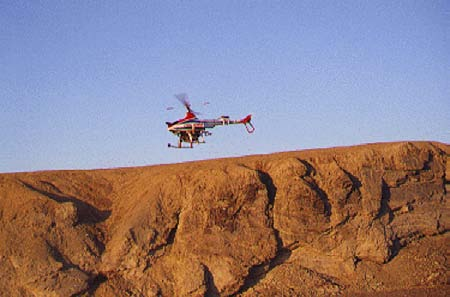
\includegraphics[scale=0.9]{figures/helicopter.png}
\caption{Carnegie Mellon University Helicopter: Autonomous Helicopter Project}
\label{automonous_drone}
\end{figure}

\section{Computer Vision in UAVs}

Computer vision is one of the most important sensors in robotics. In previous years, the complexity, computational cost, high bandwidth requirements had been the major obstacles to robust servo visual control. With the introduction of high-speed processors, low-cost digital cameras and faster graphics cards, real-time visual processing, visual servo control, and servo manipulator control has become a reality.

When one refers to visual control, in particular to visual control in autonomous aerial vehicles, one makes reference to the use of visual information obtained from image processing in order to control speed, absolute or relative position, and orientation of an aerial robot (UAV).

One of the first autonomous helicopters, figure \ref{automonous_drone}, guided by computer vision is described in [Amidi, 1996]. This vehicle combines the GPS readings with a vision system, in order to increase the precision of the state estimate for navigation. The vision system consists of a DSP (Digital Signal Processor) that provides position, velocity and attitude measurements at frequencies of the order of 10ms, which combined with the GPS and IMU (Inertial Measurement Unit)  readings increases the accuracy in estimating the attitude and position of the helicopter. 

[Bosse, 1997] focuses on the use of a camera as an additional sensor for the navigation of an autonomous helicopter. Given a sequence of images taken by a camera the estimate of 3D movement of the camera is achieved. This estimate is then merged with inertial information which is applied to help the UAV during landing process. Visual control has also been applied to miniature vehicles, in the case of a four-rotor helicopter (HUX-4) [Altug, 2003], [Altug et al., 2005] where vision is used to determine the arrangement(disposicion) of the helicopter and for the detection of objects on land. In the case of a miniature aircraft [Causey, 2003] the detection and location of the horizon is used for the lateral control of a mini UAV.

Zhang [Zhang, 2000] used an on-board camera to detect and follow a colored circle in order to control an airship. The planning of the trajectory is done in the plane of the image, which eliminates the calibration and saves computational cost. However the visual control is done by introducing the dynamics of the system (airship) while in the visual processing.

In the area of autonomous landing based on vision, recently in [Merz et al., 2004] the detection of a known pattern using computer vision and the fusion of this information with the inertial measures allows this helicopter to land in case of non-availability of GPS. In [Johnson et al., 2005] computer vision techniques are used to recover and detect safe areas for landing on an unknown terrain. Previously, artificial vision was used to autonomously land a helicopter using two different strategies [Saripalli et al., 2003a] and [Shakernia et al., 1999], but with the particularity of computer vision as the main source of information.

In the case of 3D navigation based on Habrar [Hrabar, 2006], it proposes an obstacle avoidance technique based on computer vision combining optical flow and stereoscopic vision. Experiments demonstrate the advantages of combining both techniques, which in turn combined with a path planner based on probabilistic maps allows the navigation of a stand-alone helicopter in urban environments.

This chapter has presented an overview of current works and developments in autonomous air vehicles, with particular emphasis on autonomous helicopters. The rapid development of this technology is making the state of the art progress vertiginously finding new developments and applications every day, some because of their private nature are not publicly documented. Although, the subject of helicopter control has been well studied and is being considered solved, this is not the case when using computer vision for visual control. The high requirements of reliability and robustness necessary by UAV control urges for new developments and techniques for computer vision that satisfy these demands.


\section{OpenCV}

Artificial vision is one of the main scientific disciplines when it comes to reproducing what human beings can perceive through their own physical senses in a computer. The analysis and the processing of images are one of the methods that form the basis of the artificial vision. In computing there are several techniques such as pattern search, image filtering, or projective integrals  that require complex algorithms and considerable computational effort.

One of the most used resources in the field of artificial vision is OpenCV. This is a free software library that includes various pieces of code written in C ++, C, Python, Java and Matlab. OpenCV is capable of producing more than 500 algorithms with different functionalities that cover much of the analysis of images and the well-known learning of the machine. It has a modular structure (Figure \ref{opencv_structure}) that facilitates its use when it comes to including libraries in projects. Each module differs to produce a different functionality. The main modules of OpenCV are: core, imgproc, video, calib3d, features2d, objdetect, highgui and gpu.

\begin{figure}[h!]
\centering
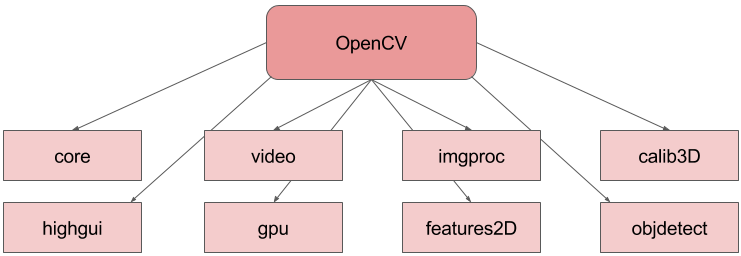
\includegraphics[scale=0.7]{figures/opencv_structure.png}
\caption{Basic components of OpenCV that form the modular structure}
\label{opencv_structure}
\end{figure}

The main objective of OpenCV is to provide tools that help people build programs related to image analysis that are increasingly sophisticated and optimal, as we can see in facial detection methods in the image (Figure \ref{image_processing}).

\begin{figure}[h!]
\centering
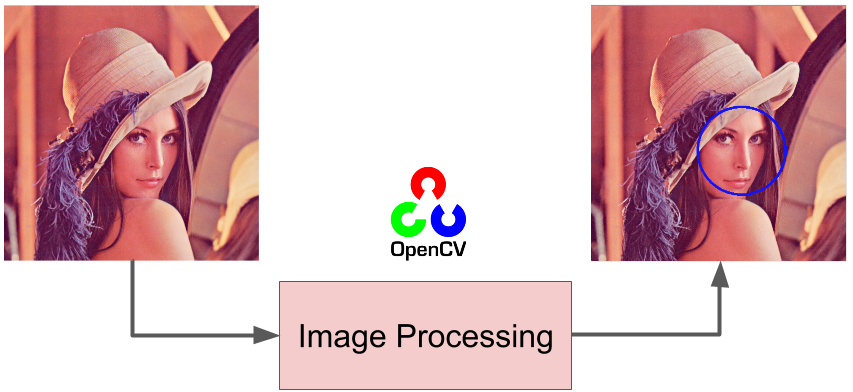
\includegraphics[scale=0.7]{figures/image_processing.png}
\caption{Example of facial detection in OpenCV with Lena Söderberg}
\label{image_processing}
\end{figure}


%\begin{figure}[h]
%\centering
%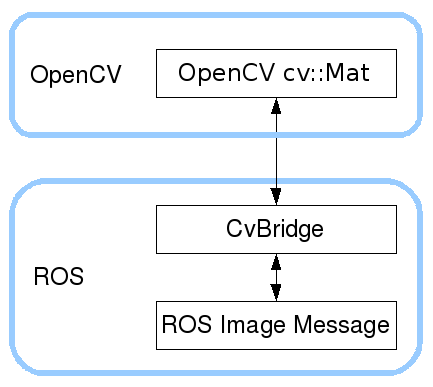
\includegraphics[scale=0.4]{figures/cv_bridge.png}
%\caption{Pipeline from a ROS image to an OpenCV image \cite{ApacheHadoop}}
%\label{HDFSArch}
%\end{figure}

\section{TLD (Tracking-Learning-Detection)}

Tracking-Learning-Detection (TLD), also known as Predator algorithm is a real-time algorithm for the tracking of unknown objects in video streams developed by Zdenek Kalal[28].

The object of interest is defined by a bounding box in a single frame and TLD simultaneously tracks the object, learns its appearance and detects it whenever it appears in the video.
By separating tracking and detection, TLD algorithm outperforms existing adaptive tracking-by-detection methods. Also, a notable reduction in the computing time is achieved by using simple features for object detection.

The TLD framework decomposes the long-term tracking task into three sub-tasks: tracking, learning and detection. Each sub-task is addressed by a single component and they operate simultaneously(see Figure \ref{tld_process}).

\begin{itemize}
\setlength{\itemsep}{-10pt}
\item \textbf{Tracker:}Follows the object through the frames.
\item \textbf{Detector:} Localizes all the appearances that have been observed so far and corrects the tracker if necessary.
\item \textbf{Learning:} Estimates the error and updates it to avoid these error in the future.
\end{itemize}

The TLD work-flow starts with the initialization, which leads to a learning step. 
Then the tracker. The diagram below shows the process:

\begin{figure}[h!]
\centering
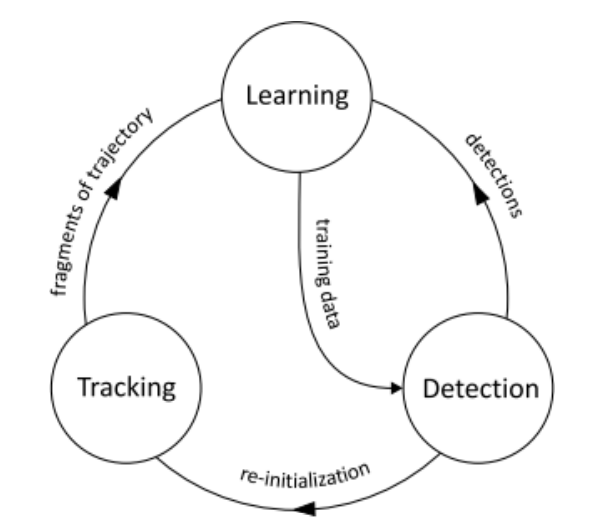
\includegraphics[scale=0.6]{figures/tld_process.png}
\caption{Block diagram of the Tracking Learning Detection algorithm}
\label{tld_process}
\end{figure}


\section{Image Recognition: TensorFlow}

\begin{figure}[h]
\centering

\includegraphics[scale=0.4]{figures/tensorflow_logo.png}
\caption{TensorFlow Logo}
\label{TensorFlow_Logo}
\end{figure}

Image recognition is a very powerful tool that is performed through automated learning. In general, it is a process that requires a very high computational complexity because it has to simulate a cognitive stimulation that exercises sensorial perception in humans, similar to gnosia.

In recent years, There has been tremendous progress in tackling these difficulties. In particular, Google has developed an automatic learning tool that uses a neural convolution network which has come to produce the same results or even improve them in comparison to human visual recognition tasks.

This tool is called TensorFlow, figure  \ref{TensorFlow_Logo}, released on the 15th of November 2015 by Google, TensorFlow is an open source library TensorFlow is an open source library that is based on a neural network system. This means that it can relate several data on the network simultaneously, in the same way as the human brain does.

%Released on the 15th of November 2015 by Google, TensorFlow is an open source library that is based on a neural network system. This means that it can relate several data on the network simultaneously, in the same way as the human brain does. 

Tensorflow's  automatic learning system specializes in voice recognition, text recognition, and image recognition. For example, you can recognize several words in the alphabet because it relates letters and phonemes. \\ Another case is that of images and texts that can be related to each other quickly thanks to the association capacity of the neural network system. According to Google, TensorFlow can be very useful for health, insurance and automotive commercial sectors. Since it released the code, several companies, Universities, and researchers use the software or have relied on it to develop applications.

\begin{figure}[h]
\centering
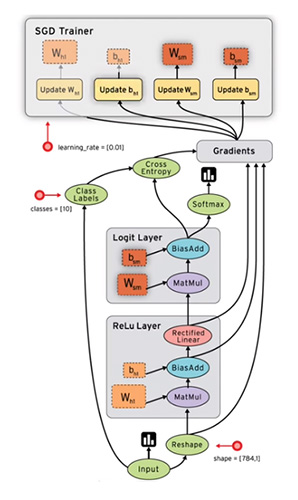
\includegraphics[scale=0.5]{figures/TensorFlow-graph.jpg}
\caption{TensorFlow graph}
\label{TensorFlow-graph}
\end{figure}

\section{Inception-V3}

Inception-v3 is a version of a TensorFlow model for image recognition, trained from the ImageNet 7 neural network. Inception-v3 has the ability to classify images into more than 1000 classes according to the degree of similarity it encounters.

This model first identifies the main characteristics of the image that we want to recognize, obtaining the contours of the figure as a function of its geometry and contrast with the background. Next, an algorithm is in charge of relating the whole geometry obtaining an abstract representation of our figure to classify.

It is at this point when the system decides to make the comparison of our figure with the model that has been trained from images that exist on the web. The model searches the database for a figure to which it corresponds in order to obtain a ranking of 5 probabilities that represent the degree of similarity. The higher the likelihood, the more correct is the classification of the image. This process can be defined as a question-and-answer system, figure \ref{neural_net}, since in order to obtain a reliable answer, all the pixels in the image are analyzed and questions are asked to the model in order to obtain a reliable result based on a logical and intuitive response.

\begin{figure}[!ht]
\centering
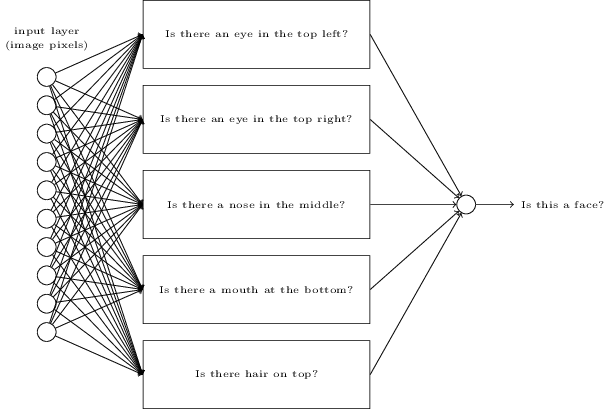
\includegraphics[scale=1.0]{figures/neural_net.png}
\caption{Architecture of a model that uses a neural network for face recognition}
\label{neural_net}
\end{figure}


%%%%%%%%%%%%%%%%%%%%%%%%%%%%%%%%%%%%%%%%%%%%%%%%%%%%%%%
%\subsection{Subsection}

%A table example is going to follow.

%\begin{table}[H]
%\centering
%\caption{This is a table template}
%\begin{tabular}{|l|c|c|c|c|c|}
%\hline
%Product & 1 & 2 & 3 & 4 & 5\\
%\hline
%Price & 124.- & 136.- & 85.- & 156.- & 23.-\\
%Guarantee [years] & 1 & 2 & - & 3 & 1\\
%Rating & 89\% & 84\% & 51\% & & 45\%\\
%\hline
%\hline
%Recommended & yes & yes & no & no & no\\
%\hline
%\end{tabular}
%\label{tab:template2}
%\end{table}
%\subsubsection{This is a subsubsection}



%%%%%%%%%%%%%%%%%%%%%%%%%%%%%%%%%%%%%%%%%%%%%%%%%%%
%
%  New template code for TAMU Theses and Dissertations starting Fall 2012.  
%  For more info about this template or the 
%  TAMU LaTeX User's Group, see http://www.howdy.me/.
%
%  Author: Wendy Lynn Turner 
%	 Version 1.0 
%  Last updated 8/5/2012
%
%%%%%%%%%%%%%%%%%%%%%%%%%%%%%%%%%%%%%%%%%%%%%%%%%%%
%%%%%%%%%%%%%%%%%%%%%%%%%%%%%%%%%%%%%%%%%%%%%%%%%%%%%%%%%%%%%%%%%%%%%%
%%                           SECTION III
%%%%%%%%%%%%%%%%%%%%%%%%%%%%%%%%%%%%%%%%%%%%%%%%%%%%%%%%%%%%%%%%%%%%%

\chapter{\uppercase{Related Work}}

%Traditonal Workflow
%Data Interpretation
%Data Visualization
%Faults Prediction
%Attributes Computation
%Execution
%HPC
%IO Scalability
%Ease to use

Tracking in video is one of the most difficult problem in computer vision as many different and varying situations such as varying illumination, change in scene, varying number of targets need to be adressed and solved. A large number of tracking methods have been proposed in literature based on the type of application in the area. Some of those methods are based on object segmentation model, motion model and probabilistic model. Lukas-Kanade [9] tracker finds the appropriate affine transformation for the features found in the local neighborhood of the current frame for a target to the features of the same target in next frame. This tracker has been widely used in literature for estimating the optical flow. Optical flow is one of the successful algorithms to find the match for the local feature of a target between two frames when the target intensity remains consistent and the target moves slowly. [32] used Lucas Kanade optical flow tracker for queue analysis at intersections. Mean shift algorithm [31] is an iterative algorithm for finding the mode of the distribution. This algorithm needs the histogram back projected image and the initial location of the target as input to initialize the tracker. The tracker in the next frame finds the best match for the histogram distribution using Bhattacharya distance. The camshift (Continuously Adaptive Meanshift) [31] applies meanshift first to find the match for the target histogram. Once the mean shift algorithm converges to the best match, Camshift updates the size of the window and fits the best fitting eclipse to the window. Again it applies meanshift over the new search window. In camshift the window size adapts accordingly to the size and the movement of the target.

\pagebreak

Motion based features are sensitive to noise. Thus, most of the motion based approach results in high false alarm rate. The state space approach better handles the multivariate, linear, non-linear and non-Gaussian processes, which thus, is often used in solving tracking problem. The state vector contains all the set of information to describe the system. As a simple example for
tracking problem, the centroid of the bounding box or object and its velocity along X−direction and Y −direction is the state of the system. The measurement vector represents the set of noisy
observations that are related to the state vector. [33] used Kalman filter for tracking multi-object. Kalman filter gives a nice Gaussian solution for the location of a target if the problem is linear in nature with added Gaussian noise. It establishes the suitable motion model for tracking. [32] used constant velocity for modeling the vehicle dynamics and estimate the track using Kalman filter. In [34] support vector machine and Kalman filtering are adopted for detection and tracking respectively.

In probabilistic model tracking problems are solved by estimating the state of the object of interest that changes over time using a sequences of noisy measurement [35]. Prokaj, J. and Medioni, G. in [30], however presented the multiple objects tracking approach based on two trackers. The first one is detection based tracker which relies on the background subtraction model and the second one is based on the target state regression tracking, which provides frame to frame tracking. In regression tracker, only the valid samples from the motion models are acquired using regressor. The main advantage of this model is that, it does not incorporate appearance model and handles the stopping target better. However, the use of two trackers in parallel increase the computational time and also as the regressor model is initialized using detector model, tracker may fails if the detector fails to detect some target of interest.

The posterior probability density function of the state of the dynamic system can be computed from the set of available noisy measurements, which can be used to estimate the optimal solution for the new state [35]. The state space model predicts the state of the state and use the measurement model (if available) to update the state from a bunch of noisy predicted state using the Bayes theorem. In [30] authors described the tracking framework in wide area surveillance from the fusion of color and thermal imagery working under the Bayesian framework (particle filtering).
They defined the state of each pedestrian with its bounding box location and 2D color histogram. Particle filter is computationally expensive but a robust form of tracking which can easily handle the situation even when the system is non-linear and non-Gaussian unlike for Kalman filter. Some of the randomly distributed particles will capture the underlying model and the probability distribution of the target.

In multi-target tracking target arise at the random time and space, exists for the random length of time. It is important to associate the right measurement to right target track. Data association is a major problem in multiple target tracking. One of the methods for associating the data is the greedy nearest neighbor method. For a target it associates the measurement which is closest to the predicted position [32]. [33] also uses the greedy nearest neighbor method for target tracking but also incorporate the area of the track and the measurement in the cost function.
%%%%%%%%%%%%%%%%%%%%%%%%%%%%%%%%%%%%%%%%%%%%%%%%%%
%
%  New template code for TAMU Theses and Dissertations starting Fall 2012.  
%  For more info about this template or the 
%  TAMU LaTeX User's Group, see http://www.howdy.me/.
%
%  Author: Wendy Lynn Turner 
%	 Version 1.0 
%  Last updated 8/5/2012
%
%%%%%%%%%%%%%%%%%%%%%%%%%%%%%%%%%%%%%%%%%%%%%%%%%%%
%%%%%%%%%%%%%%%%%%%%%%%%%%%%%%%%%%%%%%%%%%%%%%%%%%%%%%%%%%%%%%%%%%%%%%
%%                           SECTION IV
%%%%%%%%%%%%%%%%%%%%%%%%%%%%%%%%%%%%%%%%%%%%%%%%%%%%%%%%%%%%%%%%%%%%%

\chapter{\uppercase{Design}}

The primary goal of this thesis is to implement an object detection and tracking system using one of the most well-known visual tracking algorithms and machine learning frameworks from the computer vision field: TensorFlow, YOLO, TLD, and OpenCV. We will make some modifications and adaptations to our use case to be able to identify and follow an object. This chapter introduces the software architecture design and main functionalities of this system.

\section{Software Architecture Design}

For developing the visual tracking system, we need to do more programming work in addition of the object detection and tracking algorithms. In order to achieve the proposed goal, we need to implement a program capable of tracking a person or object, determine its trajectory and follow it by using the drone’s on-board camera. We are going to implement this program using the Dronekit library provided as part of the SDK Package by 3DRobotics, which will be embedded into our laptop/Mobile device. TensorFlow for python as a programming language and 3DR Solo SDK packages --Dronekit-- are used to communicate with the drone. Using DroneKit allows developers to write web-based drone apps, mobile apps and as well as to create apps that run on an onboard companion computer and communicate with the ArduPilot flight controller using a low-latency link (written in Python). The API communicates with vehicles over MAVLink. It provides programmatic access to a connected vehicle’s telemetry, state and parameter information, and enables both mission management and direct control over vehicle movement and operations such as commanding the drone to fly certain paths, follow a GPS target, control camera gimbals in addition to also allowing developers to log all of the drone’s movements for later analysis.

We are going to re-implement one of the most powerful and fastest object detection algorithms in computer vision using python and TensorFlow; YOLO(You Only Look Once)-- by [Redmon et. al], as for integrating tracking into our system, TLD(Tracking Learn Detection) by [Zdenek et. al] will be used. These algorithms are going to help us build the functions for detecting and following the object while it is moving in front of the drone's on-board camera.

\begin{figure}[h]
\centering
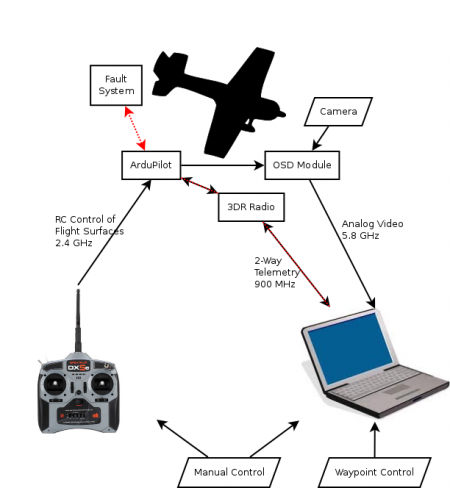
\includegraphics[scale=0.9]{figures/base_station_architecture_ardupilot.png}
\caption{Communication pipeline from Mobile device to UAV}
\label{base_station_architecture_ardupilot}
\end{figure}


\section{Interfaces and functionality: Communication between OpenCV and ROS}

Most of the artificial vision is given by the sensors of the models that we define. In order to manipulate the information we obtain through the sensors, ROS has a set of OpenCV libraries that provide the necessary tools to transform the images that are captured through the optical focus of the drone camera. In addition, it includes a large number of algorithms for odometry visual, augmented reality, machine learning and detection and recognition of objects that facilitate the use of drone controllers.

The images that are captured through the video stream of the camera are given by the topic that defines the sensor of the camera of the drone. These images are sent in a ROS sensor\_msgs/Image format. In order to manipulate these images in OpenCV it is necessary to convert them into a cv::Mat format, since it is the only compatible one. For this, there is a ROS library called cv\_bridge, which allows the transformation of ROS image to OpenCV image or otherwise OpenCV image to ROS image.


\begin{figure}[h!]
\centering
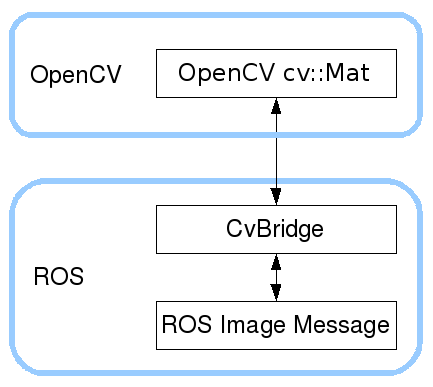
\includegraphics[scale=0.6]{figures/cv_bridge.png}
\caption{Pipeline from a ROS image to an OpenCV image}
\end{figure}

The conversion process (Algorithm 2.1) begins at the moment when our program captures the images produced by the topic that obtains the data of the camera and they begin to receive in sensor\_msgs::ImageConstPtr format. Then the transformation is done from the toCvCopy method that receives as a parameter the ROS message and the type of encoding that in this case is BGR8. As a result we obtain a structure which can be accessed in the Mat format image with CvImagePtr to image.


\section{Programming Language}

The host programming language for the Dronekit SDK as well as TensorFlow and thereby, the language that we will use to build the different functionalities of the proposed application is Python.  Python is a general purpose programming language created in the late 1980s, it is used by thousands of people to do things from testing microchips at Intel, to powering Instagram, to building video games. Python is small, very closely resembles the English language, and has hundreds of existing third-party libraries especially in computer vision hence our choice to use it since it will make our tasks simpler to perform.

\begin{figure}[h]
\centering

\includegraphics[scale=0.6]{figures/python.png}
\caption{Python Logo}
\end{figure}


%%%%%%%%%%%%%%%%%%%%%%%%%%%%%%%%%%%%%%%%%%%%%%%%%%
%
%  New template code for TAMU Theses and Dissertations starting Fall 2012.  
%  For more info about this template or the 
%  TAMU LaTeX User's Group, see http://www.howdy.me/.
%
%  Author: Wendy Lynn Turner 
%	 Version 1.0 
%  Last updated 8/5/2012
%
%%%%%%%%%%%%%%%%%%%%%%%%%%%%%%%%%%%%%%%%%%%%%%%%%%%
%%%%%%%%%%%%%%%%%%%%%%%%%%%%%%%%%%%%%%%%%%%%%%%%%%%%%%%%%%%%%%%%%%%%%%
%%                           SECTION IV
%%%%%%%%%%%%%%%%%%%%%%%%%%%%%%%%%%%%%%%%%%%%%%%%%%%%%%%%%%%%%%%%%%%%%

\chapter{\uppercase{Implementation}}

The system developed in this thesis  is a TensorFlow re-implementation of  YOLO which is a fast and accurate real time object detection system originally designed by [Redmon et al., 2012]. In our implementation, we perform predictions by leveraging weights that have been trained for a long time on GPUs using ImageNet data, which is a public dataset containing millions of natural images. In our implementation, we trained the model using TensorFlow to export the graph or trained model generated using a tool called protocol buffer that  allows for easily taking advantage of the model classes in other platforms and programming languages such as mobile platforms like iOS using swift or android using java. Furthermore, we want to be able to perform real-time object tracking in live video feeds from onboard cameras on UAVs.

\section{Hardware}
We use an Nvidia GTX 1060 in our setup to benefit from faster training times in deep learning frameworks. Particularly,  TensorFlow which supports CUDA and cuDNN making neural network training significantly faster. 16GB memory to afford adding more layers to our neural network model if  required. A 256 GB SSD is used for quick access to applications and disk space for small data such as documents. A 1TB HDD is used for larger data such as stored, trained network parameters, and datasets, which quickly sum up due to copies and modifications. The CPU used is an Intel Quad-Core i7 6700HQ @ 2.6Ghz.

\pagebreak
\section{YOLO (You Only Look Once)}

YOLO is a convolutional neural network that can predict multiple-box positions and categories at once, enabling end-to-end target detection and recognition. The biggest of YOLO advantage is speed. In fact, the nature of the target detection is regression, so a CNN that implements the regression function does not require a complex design process.

YOLO avoids computationally expensive region proposal steps that detectors like Fast R-CNN[4] and Faster-RCNN[14] require. The advantage of doing so is to better distinguish between the target and the background area, compared to the use of proposal training Fast-R-CNN often the background area for a specific target. Of course, YOLO in the detection speed at the same time sacrifice some of the accuracy. 

\begin{figure}[h]
\centering
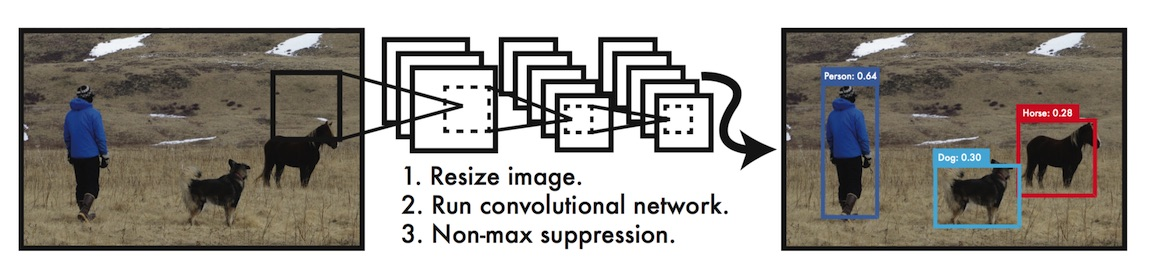
\includegraphics[scale=0.35]{figures/yolo_working.jpg}
\caption{YOLO detection system process}
\label{yolo_working}
\end{figure}

Figure \ref{yolo_working} shows the overall structure of the network :

\begin{enumerate}
\setlength{\itemsep}{-10pt}
\item Resize the image to 448 x 448.
\item Run a single convolution network.
\item Get the location and category of the object.
\end{enumerate}

\section{YOLO Network Design}

YOLO uses unified detection which unites the separate components of object detection into a single neural network. This network uses features from the entire image to predict each bounding box. This design differentiates YOLO from other methods and enables end-to-end training with real-time speeds while maintaining high average precision.  Unified detection system uses S x S grid cells and predicts B bounding boxes for each cells. Each bounding boxes produces 5 predictions: \textbf{ x},\textbf{ y}, \textbf{w}, \textbf{ h}, and confidence. The \textbf{(x,y)} is the coordinates of the center of box relative to the bounds of the grid cell. \textbf{(w,h)} is the width and height of the bounding box. The confidence score is calculated by the probability of the object multiplied by the intersection of the union of ground truth and prediction labels. Then each grid cell produce the conditional class probabilities. These probabilities are used at test time to produce the final predictions.

The final class-specific confidence scores are calculated by multiplying the conditional class probabilities with the individual box confidence predictions. The neural network architectural design includes two main components: feature extraction and prediction. The feature extraction consists of 24 convolutional layers to obtain the final 7 x 7 x 1024 activation map. This image information is passed to prediction section that has 2 fully connected layers. The probability and coordinates are produced by the last FC layer in the 7 x 7 x 30 tensor of predictions.\\

\newpage
The architecture diagram is shown in figure \ref{yolo_model} and figure \ref{yolo_net}. 

\begin{figure}[h]
\setlength{\belowcaptionskip}{-30pt}
\centering
%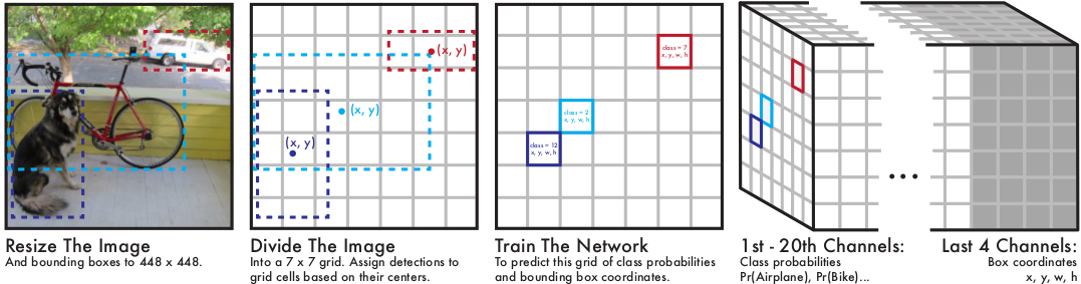
\includegraphics[scale=0.4]{figures/yolo_model.png}
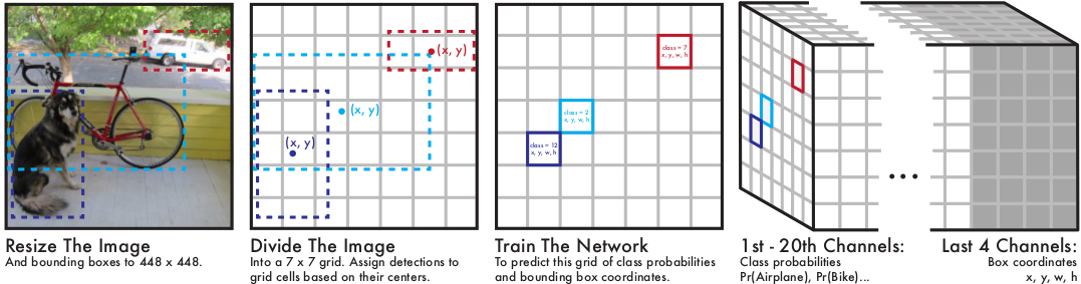
\includegraphics[width=10cm,height=12cm,keepaspectratio]{figures/yolo_model.png}
\caption{YOLO neural network prediction process}
\label{yolo_model}
\end{figure}

\begin{figure}[h]
\setlength{\belowcaptionskip}{-30pt}
\centering
%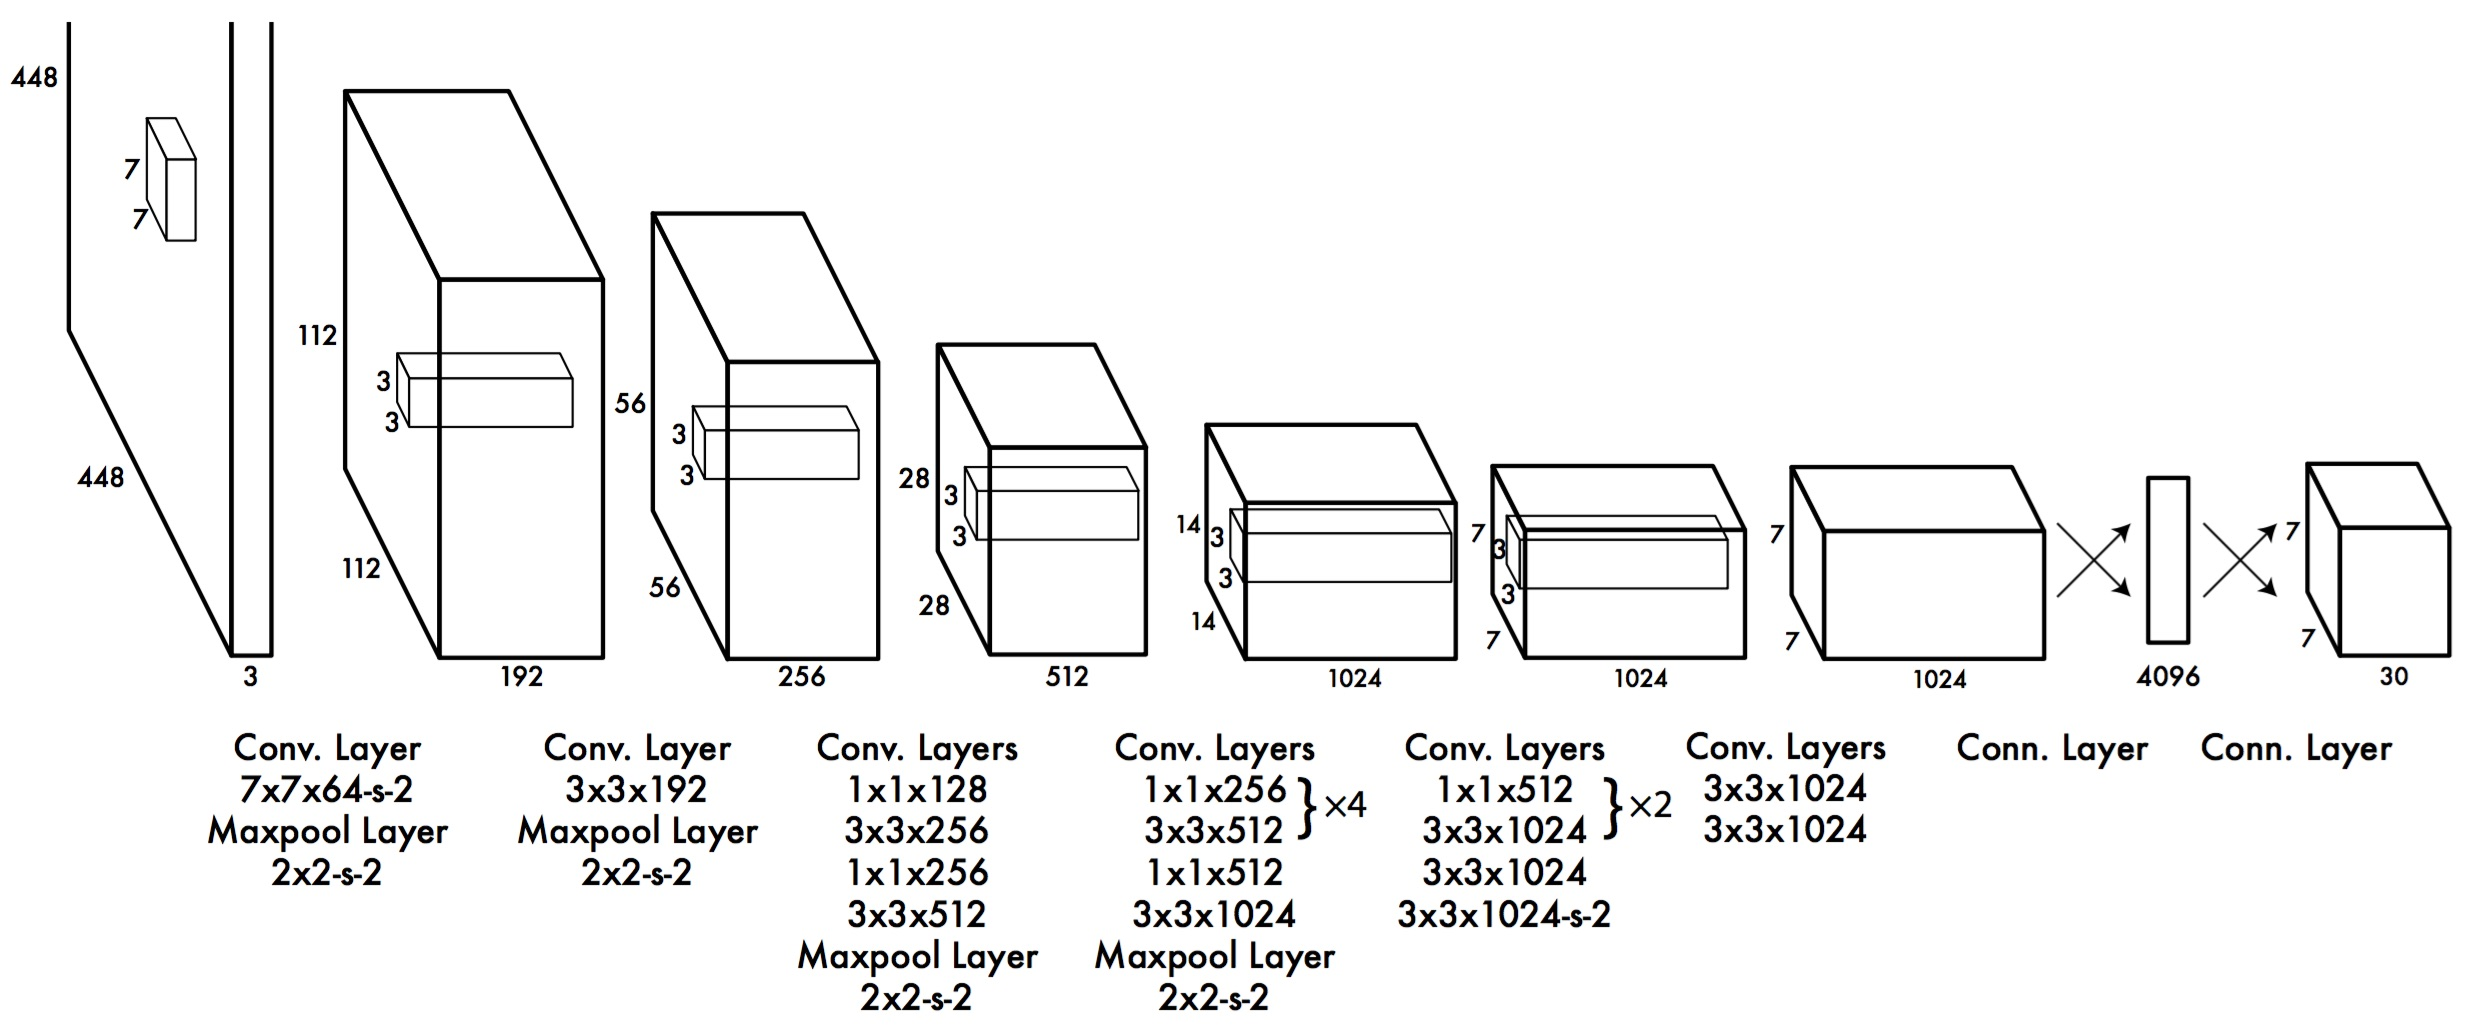
\includegraphics[scale=0.2]{figures/yolo_net.jpg}
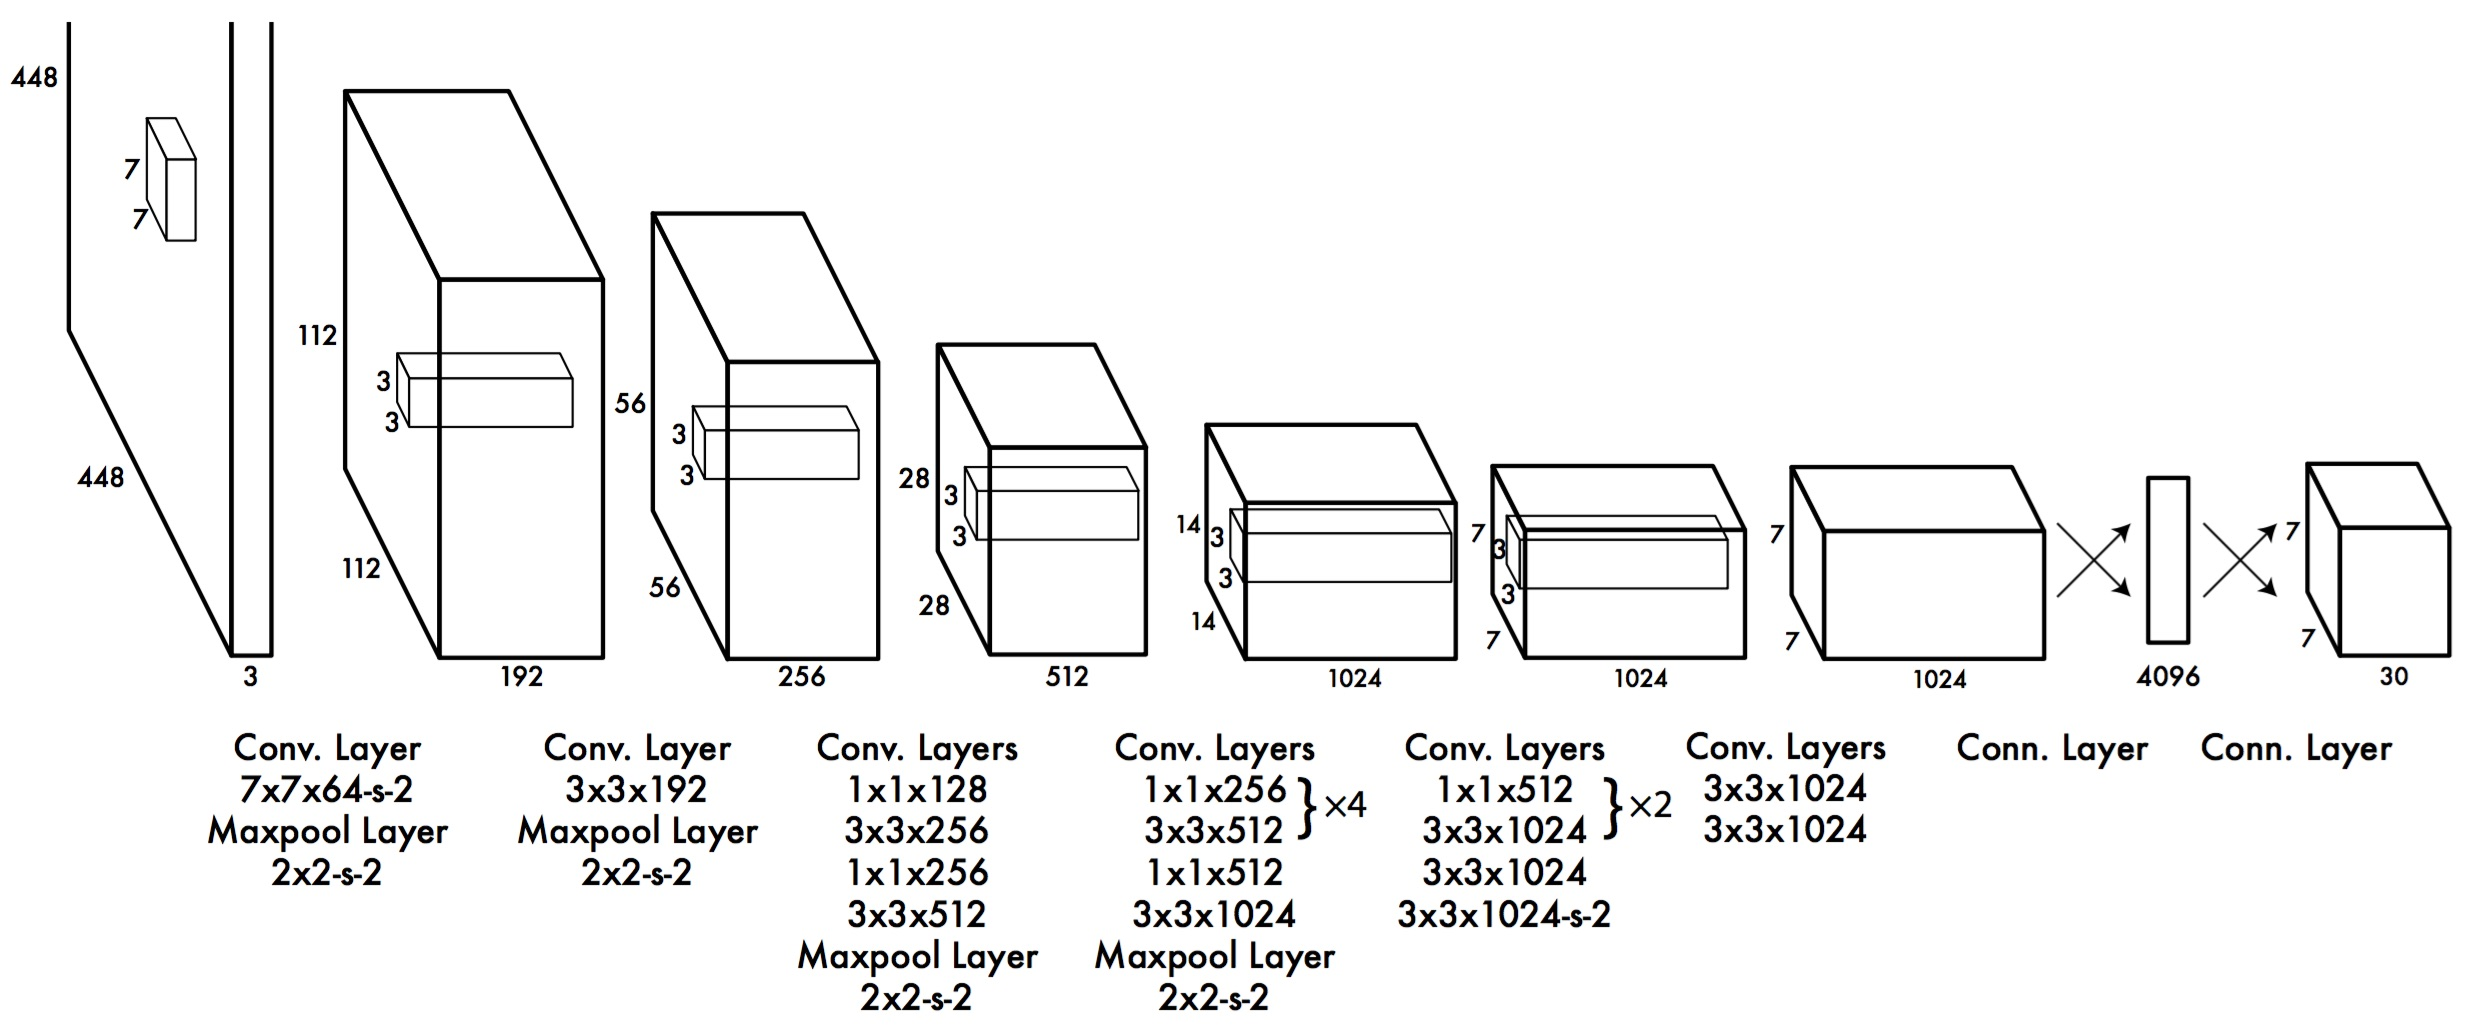
\includegraphics[width=12cm,height=10cm,keepaspectratio]{figures/yolo_net.jpg}
\caption{YOLO neural network structure}
\label{yolo_net}
\end{figure}

\vspace{10mm}
\section{ System Architecture Overview}

As it has been mentioned earlier, the system proposed in this thesis is built on top of the YOLO Architecture using our  TensorFlow implemented port  which will help in making our training more efficient and faster. We must note that YOLO is designed to process images in sequence. Therefore, it has no concept of temporal or spatial continuity between sequential frames in a video. For instance, while video frames may be fed into YOLO sequentially, YOLO cannot determine which object detected in one frame corresponds to the same object in the next frame.  Our task is to re-implement, train, and test  YOLO using TensorFlow and TLD(Tracking-Learning-Detection) so that it can track objects within a video in real-time and build  an application for a UAV/drone that uses a open source SDK to integrate our computer vision algorithm in ground station and the UAV to identify and track objects transmitted on a live video feed.

Figure \ref{our_app_2} shows a diagram on how we implement YOLO in TensorFlow to detect objects in video files, pictures, and live video feeds:

\begin{figure}[h]
\setlength{\belowcaptionskip}{-30pt}
\centering

\includegraphics[scale=0.3]{figures/our_app_2.png}
\caption{YOLO in TensorFlow implementation diagram}
\label{our_app_2}
\end{figure}

\vspace{10mm}

Figure \ref{our_architecture} shows an overview on how our system is implemented. First, a video sequence is given as an input,  in our case, we will use a live video feed from a drone's camera.

\begin{figure}[h]
\setlength{\belowcaptionskip}{-10pt}
\centering

\includegraphics[scale=0.3]{figures/our_app.png}
\caption{Block Diagram of the system architechture}
\label{our_architecture}
\end{figure}

\vspace{200mm}

The code snippet below shows how we access live video feed from a drone's camera and download it to our mobile device:

\vspace{5mm}
\begin{lstlisting}
// videofeed.py
import cv2
import numpy as np
import dronekit

// Create a VideoCapture object
cap = cv2.VideoCapture('./sololink.sdp')
// Check if camera opened successfully
if (cap.isOpened() == False): 
  print("Unable to read camera feed")
// Default resolutions of the frame are obtained.The default resolutions are system dependent.
// We convert the resolutions from float to integer.
frame_width = int(cap.get(3))
frame_height = int(cap.get(4))
// Define the codec and create VideoWriter object.The output is stored in 'outpy.avi' file.
out = cv2.VideoWriter('outpy.avi',cv2.VideoWriter_fourcc('M','J','P','G'), 10, (frame_width,frame_height))
while(True):
  ret, frame = cap.read()
  if ret == True: 
    // Write the frame into the file 'output.avi'
    out.write(frame)
    // Display the resulting frame    
    cv2.imshow('frame',frame)
    // Press Q on keyboard to stop recording
    if cv2.waitKey(1) & 0xFF == ord('q'):
      break
  // Break the loop
  else:
    break 
// When everything done, release the video capture and video write objects
cap.release()
out.release()
// Closes all the frames
cv2.destroyAllWindows() 
// videofeed.py
\end{lstlisting}

%\vspace{14mm}
\pagebreak
Detecting and classifying an object from the video feed or video sequence is done using our TensorFlow implementation of YOLO. The code snippet below shows how we proceed to implement our object detection algorithm.

\vspace{5mm}

\begin{lstlisting}
// detect.py
import os
import argparse
import configparser
import importlib
import itertools
from PIL import Image, ExifTags
import numpy as np
import matplotlib.pyplot as plt
import matplotlib.patches as patches
import tensorflow as tf
import tensorflow.contrib.slim as slim
import utils.preprocess
import utils.postprocess

def std(image):
    return utils.preprocess.per_image_standardization(image)

def darknet(image):
    return image / 255.

def read_image(path):
    image = Image.open(path)
    for key in ExifTags.TAGS.keys():
        if ExifTags.TAGS[key] == 'Orientation':
            break
    try:
        exif = dict(image._getexif().items())
    except AttributeError:
        return image
    if exif[key] == 3:
        image = image.rotate(180, expand=True)
    elif exif[key] == 6:
        image = image.rotate(270, expand=True)
    elif exif[key] == 8:
        image = image.rotate(90, expand=True)
    return image

def detect(sess, model, names, image, path):
    preprocess = eval(args.preprocess)
    _, height, width, _ = image.get_shape().as_list()
    _image = read_image(path)
    image_original = np.array(np.uint8(_image))
    if len(image_original.shape) == 2:
        image_original = np.repeat(np.expand_dims(image_original, -1), 3, 2)
    image_height, image_width, _ = image_original.shape
    image_std = preprocess(np.array(np.uint8(_image.resize((width, height)))).astype(np.float32))
    feed_dict = {image: np.expand_dims(image_std, 0)}
    tensors = [model.conf, model.xy_min, model.xy_max]
    conf, xy_min, xy_max = sess.run([tf.check_numerics(t, t.op.name) for t in tensors], feed_dict=feed_dict)
    boxes = utils.postprocess.non_max_suppress(conf[0], xy_min[0], xy_max[0], args.threshold, args.threshold_iou)
    scale = [image_width / model.cell_width, image_height / model.cell_height]
    fig = plt.figure()
    ax = fig.gca()
    ax.imshow(image_original)
    colors = [prop['color'] for _, prop in zip(names, itertools.cycle(plt.rcParams['axes.prop_cycle']))]
    cnt = 0
    for _conf, _xy_min, _xy_max in boxes:
        index = np.argmax(_conf)
        if _conf[index] > args.threshold:
            wh = _xy_max - _xy_min
            _xy_min = _xy_min * scale
            _wh = wh * scale
            linewidth = min(_conf[index] * 10, 3)
            ax.add_patch(patches.Rectangle(_xy_min, _wh[0], _wh[1], linewidth=linewidth, edgecolor=colors[index], facecolor='none'))
            ax.annotate(names[index] + ' (%.1f%%)' % (_conf[index] * 100), _xy_min, color=colors[index])
            cnt += 1
    fig.canvas.set_window_title('%d objects detected' % cnt)
    ax.set_xticks([])
    ax.set_yticks([])
    return fig

def main():
    model = config.get('config', 'model')
    yolo = importlib.import_module('model.' + model)
    width = config.getint(model, 'width')
    height = config.getint(model, 'height')
    with tf.Session() as sess:
        image = tf.placeholder(tf.float32, [1, height, width, 3], name='image')
        builder = yolo.Builder(args, config)
        builder(image)
        global_step = tf.contrib.framework.get_or_create_global_step()
        model_path = tf.train.latest_checkpoint(utils.get_logdir(config))
        tf.logging.info('load ' + model_path)
        slim.assign_from_checkpoint_fn(model_path, tf.global_variables())(sess)
        tf.logging.info('global_step=%d' % sess.run(global_step))
        path = os.path.expanduser(os.path.expandvars(args.path))
        if os.path.isfile(path):
            detect(sess, builder.model, builder.names, image, path)
            plt.show()
        else:
            for dirpath, _, filenames in os.walk(path):
                for filename in filenames:
                    if os.path.splitext(filename)[-1].lower() in args.exts:
                        _path = os.path.join(dirpath, filename)
                        print(_path)
                        detect(sess, builder.model, builder.names, image, _path)
                        plt.show()

def make_args():
    parser = argparse.ArgumentParser()
    parser.add_argument('path', help='input image path')
    parser.add_argument('-c', '--config', nargs='+', default=['config.ini'], help='config file')
    parser.add_argument('-p', '--preprocess', default='std', help='the preprocess function')
    parser.add_argument('-t', '--threshold', type=float, default=0.3)
    parser.add_argument('--threshold_iou', type=float, default=0.4, help='IoU threshold')
    parser.add_argument('-e', '--exts', nargs='+', default=['.jpg', '.png'])
    parser.add_argument('--level', default='info', help='logging level')
    return parser.parse_args()

if __name__ == '__main__':
    args = make_args()
    config = configparser.ConfigParser()
    utils.load_config(config, args.config)
    if args.level:
        tf.logging.set_verbosity(args.level.upper())
    main()
// detect.py
\end{lstlisting}

\vspace{5mm}
Using OpenCV feature extraction algorithm, we track a set of features across the video sequence. Once the features have been detected in the object throughout the video frames, it will identify the same points accross the live video feed. To track the detected object over time,  we use TLD (Tracking-Detection-Learning) algorithm to learn the objects appearance and detect it whenever it moves or appears in the video feed.

\vspace{5mm}

\begin{lstlisting}
//tracker.py
//Tracking using TLD in OpenCV
import numpy as np
import cv2
import sys

if len(sys.argv) != 2:
    print('Input video name is missing')
    exit()

print('Select 3 tracking targets')

cv2.namedWindow("tracking")
camera = cv2.VideoCapture(sys.argv[1])
tracker = cv2.MultiTracker_create()
init_once = False

ok, image=camera.read()
if not ok:
    print('Failed to read video')
    exit()

bbox1 = cv2.selectROI('tracking', image)
bbox2 = cv2.selectROI('tracking', image)
bbox3 = cv2.selectROI('tracking', image)

while camera.isOpened():
    ok, image=camera.read()
    if not ok:
        print 'no image to read'
        break

    if not init_once:
        ok = tracker.add(cv2.TrackerMIL_create(), image, bbox1)
        ok = tracker.add(cv2.TrackerMIL_create(), image, bbox2)
        ok = tracker.add(cv2.TrackerMIL_create(), image, bbox3)
        init_once = True

    ok, boxes = tracker.update(image)
    print ok, boxes

    for newbox in boxes:
        p1 = (int(newbox[0]), int(newbox[1]))
        p2 = (int(newbox[0] + newbox[2]), int(newbox[1] + newbox[3]))
        cv2.rectangle(image, p1, p2, (200,0,0))

    cv2.imshow('tracking', image)
    k = cv2.waitKey(1)
    if k == 27 : break # esc presse
//tracker.py
\end{lstlisting}

\vspace{5mm}
\section{Training Our Network: Dataset}

Even though, our ultimate goal is to use a dataset that offers more advantages to our application in terms of training as well as testing such as COCO. Initially and for faster prototyping, we have used the PASCAL VOC dataset to train and test the functionality of our network. This training data consists of a set of images; each image has an annotation file giving a bounding box with coordinates and object class label for each object in one of  twenty classes present in the image.

The data has been split into 50\% for training/validation and 50\% for testing. The distributions of images and objects by class are approximately equal across the training/validation and test sets. In total there are 9,963 images, containing 24,640 annotated objects.

The CNN learns high-quality, hierarchical features automatically, eliminating the need for hand-selected features.

\vspace{5mm}
Below, a code snippet shows how we implement training for our network in figure \ref{retrained_model}:

\begin{lstlisting}
//train.py
import os
import argparse
import configparser
import importlib
import shutil
import time
import inspect
import multiprocessing
import tensorflow as tf
import tensorflow.contrib.slim as slim
import utils.data


def summary_scalar(config):
    try:
        reduce = eval(config.get('summary', 'scalar_reduce'))
        for t in utils.match_tensor(config.get('summary', 'scalar')):
            name = t.op.name
            if len(t.get_shape()) > 0:
                t = reduce(t)
                tf.logging.warn(name + ' is not a scalar tensor, reducing by ' + reduce.__name__)
            tf.summary.scalar(name, t)
    except (configparser.NoSectionError, configparser.NoOptionError):
        tf.logging.warn(inspect.stack()[0][3] + ' disabled')


def summary_image(config):
    try:
        for t in utils.match_tensor(config.get('summary', 'image')):
            name = t.op.name
            channels = t.get_shape()[-1].value
            if channels not in (1, 3, 4):
                t = tf.expand_dims(tf.reduce_sum(t, -1), -1)
            tf.summary.image(name, t, config.getint('summary', 'image_max'))
    except (configparser.NoSectionError, configparser.NoOptionError):
        tf.logging.warn(inspect.stack()[0][3] + ' disabled')


def summary_histogram(config):
    try:
        for t in utils.match_tensor(config.get('summary', 'histogram')):
            tf.summary.histogram(t.op.name, t)
    except (configparser.NoSectionError, configparser.NoOptionError):
        tf.logging.warn(inspect.stack()[0][3] + ' disabled')


def summary(config):
    summary_scalar(config)
    summary_image(config)
    summary_histogram(config)


def get_optimizer(config, name):
    section = 'optimizer_' + name
    return {
        'adam': lambda learning_rate: tf.train.AdamOptimizer(learning_rate, config.getfloat(section, 'beta1'), config.getfloat(section, 'beta2'), config.getfloat(section, 'epsilon')),
        'adadelta': lambda learning_rate: tf.train.AdadeltaOptimizer(learning_rate, config.getfloat(section, 'rho'), config.getfloat(section, 'epsilon')),
        'adagrad': lambda learning_rate: tf.train.AdagradOptimizer(learning_rate, config.getfloat(section, 'initial_accumulator_value')),
        'momentum': lambda learning_rate: tf.train.MomentumOptimizer(learning_rate, config.getfloat(section, 'momentum')),
        'rmsprop': lambda learning_rate: tf.train.RMSPropOptimizer(learning_rate, config.getfloat(section, 'decay'), config.getfloat(section, 'momentum'), config.getfloat(section, 'epsilon')),
        'ftrl': lambda learning_rate: tf.train.FtrlOptimizer(learning_rate, config.getfloat(section, 'learning_rate_power'), config.getfloat(section, 'initial_accumulator_value'), config.getfloat(section, 'l1_regularization_strength'), config.getfloat(section, 'l2_regularization_strength')),
        'gd': lambda learning_rate: tf.train.GradientDescentOptimizer(learning_rate),
    }[name]


def main():
    model = config.get('config', 'model')
    logdir = utils.get_logdir(config)
    if args.delete:
        tf.logging.warn('delete logging directory: ' + logdir)
        shutil.rmtree(logdir, ignore_errors=True)
    cachedir = utils.get_cachedir(config)
    with open(os.path.join(cachedir, 'names'), 'r') as f:
        names = [line.strip() for line in f]
    width = config.getint(model, 'width')
    height = config.getint(model, 'height')
    cell_width, cell_height = utils.calc_cell_width_height(config, width, height)
    tf.logging.warn('(width, height)=(%d, %d), (cell_width, cell_height)=(%d, %d)' % (width, height, cell_width, cell_height))
    yolo = importlib.import_module('model.' + model)
    paths = [os.path.join(cachedir, profile + '.tfrecord') for profile in args.profile]
    num_examples = sum(sum(1 for _ in tf.python_io.tf_record_iterator(path)) for path in paths)
    tf.logging.warn('num_examples=%d' % num_examples)
    with tf.name_scope('batch'):
        image_rgb, labels = utils.data.load_image_labels(paths, len(names), width, height, cell_width, cell_height, config)
        with tf.name_scope('per_image_standardization'):
            image_std = tf.image.per_image_standardization(image_rgb)
        batch = tf.train.shuffle_batch((image_std,) + labels, batch_size=args.batch_size,
            capacity=config.getint('queue', 'capacity'), min_after_dequeue=config.getint('queue', 'min_after_dequeue'),
            num_threads=multiprocessing.cpu_count()
        )
    global_step = tf.contrib.framework.get_or_create_global_step()
    builder = yolo.Builder(args, config)
    builder(batch[0], training=True)
    with tf.name_scope('total_loss') as name:
        builder.create_objectives(batch[1:])
        total_loss = tf.losses.get_total_loss(name=name)
    variables_to_restore = slim.get_variables_to_restore(exclude=args.exclude)
    with tf.name_scope('optimizer'):
        try:
            decay_steps = config.getint('exponential_decay', 'decay_steps')
            decay_rate = config.getfloat('exponential_decay', 'decay_rate')
            staircase = config.getboolean('exponential_decay', 'staircase')
            learning_rate = tf.train.exponential_decay(args.learning_rate, global_step, decay_steps, decay_rate, staircase=staircase)
            tf.logging.warn('using a learning rate start from %f with exponential decay (decay_steps=%d, decay_rate=%f, staircase=%d)' % (args.learning_rate, decay_steps, decay_rate, staircase))
        except (configparser.NoSectionError, configparser.NoOptionError):
            learning_rate = args.learning_rate
            tf.logging.warn('using a staionary learning rate %f' % args.learning_rate)
        optimizer = get_optimizer(config, args.optimizer)(learning_rate)
        tf.logging.warn('optimizer=' + args.optimizer)
        train_op = slim.learning.create_train_op(total_loss, optimizer, global_step,
            clip_gradient_norm=args.gradient_clip, summarize_gradients=config.getboolean('summary', 'gradients'),
        )
    if args.transfer:
        path = os.path.expanduser(os.path.expandvars(args.transfer))
        tf.logging.warn('transferring from ' + path)
        init_assign_op, init_feed_dict = slim.assign_from_checkpoint(path, variables_to_restore)
        def init_fn(sess):
            sess.run(init_assign_op, init_feed_dict)
            tf.logging.warn('transferring from global_step=%d, learning_rate=%f' % sess.run((global_step, learning_rate)))
    else:
        init_fn = lambda sess: tf.logging.warn('global_step=%d, learning_rate=%f' % sess.run((global_step, learning_rate)))
    summary(config)
    tf.logging.warn('tensorboard --logdir ' + logdir)
    slim.learning.train(train_op, logdir, master=args.master, is_chief=(args.task == 0),
        global_step=global_step, number_of_steps=args.steps, init_fn=init_fn,
        summary_writer=tf.summary.FileWriter(os.path.join(logdir, args.logname)),
        save_summaries_secs=args.summary_secs, save_interval_secs=args.save_secs
    )


def make_args():
    parser = argparse.ArgumentParser()
    parser.add_argument('-c', '--config', nargs='+', default=['config.ini'], help='config file')
    parser.add_argument('-t', '--transfer', help='transferring model from a .ckpt file')
    parser.add_argument('-e', '--exclude', nargs='+', help='exclude variables while transferring')
    parser.add_argument('-p', '--profile', nargs='+', default=['train', 'val'])
    parser.add_argument('-s', '--steps', type=int, default=None, help='max number of steps')
    parser.add_argument('-d', '--delete', action='store_true', help='delete logdir')
    parser.add_argument('-b', '--batch_size', default=8, type=int, help='batch size')
    parser.add_argument('-o', '--optimizer', default='adam')
    parser.add_argument('-n', '--logname', default=time.strftime('%Y-%m-%d_%H-%M-%S'), help='the name for TensorBoard')
    parser.add_argument('-g', '--gradient_clip', default=0, type=float, help='gradient clip')
    parser.add_argument('-lr', '--learning_rate', default=1e-6, type=float, help='learning rate')
    parser.add_argument('--seed', type=int, default=None)
    parser.add_argument('--summary_secs', default=30, type=int, help='seconds to save summaries')
    parser.add_argument('--save_secs', default=600, type=int, help='seconds to save model')
    parser.add_argument('--level', help='logging level')
    parser.add_argument('--master', default='', help='master address')
    parser.add_argument('--task', type=int, default=0, help='task ID')
    return parser.parse_args()

if __name__ == '__main__':
    args = make_args()
    config = configparser.ConfigParser()
    utils.load_config(config, args.config)
    if args.level:
        tf.logging.set_verbosity(args.level.upper())
    main()
//train.py
\end{lstlisting}

\vspace{5mm}
\begin{figure}[h]
\setlength{\belowcaptionskip}{-30pt}
\centering
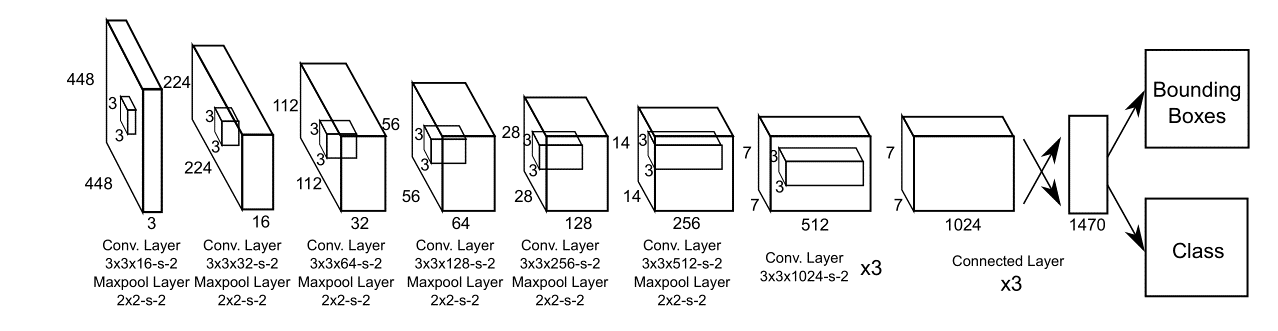
\includegraphics[scale=0.4]{figures/retrained_model.png}
\caption{Model trained  using PASCAL VOC with TensorFlow}
\label{retrained_model}
\end{figure}

\newpage
\section{Migrating Model to C++, JAVA, SWIFT, OBJECTIVE-C}

This is a tricky process to do since there is no official support for loading variables in C++ API. Google suggests assigning the trained weights as constants into the graph and save it down as a .pb (protobuf) file. However, this will double the necessary size of this file, which is very undesirable in, say, building mobile applications, for further information, refer to the official documentation forTensorflow C++ API  \url{https://www.tensorflow.org/api_docs/cc/}

To avoid this, one would have to build the graph all over again with all Variables replaced by Constants (we wouldn’t train any Deep Learning model on mobile device any time soon). Unfortunately, since there is no variable in this new graph, Tensorflow does not allow the convenient checkpointing, so one would need to resort to  \textbf{./binaries/.} while building this constant graph. In short, in order to produce a protobuf graph with optimal size for use in C++ , JAVA, and Objective-C++ API, one would need to use .weights files stored in \textbf{./binaries/.}

\vspace{5mm}
Below a snippet for exporting aour graph for use on mobile platforms:

\vspace{5mm}
\begin{lstlisting}
def savepb(self):
//Create a standalone const graph def
//So that C++ can load and run it.
//What's good abt it?
//1. Don't double the necessary size
//2. Convert on the fly - at any point you want
	
		darknet_ckpt = self.darknet
		flags_ckpt = self.FLAGS
		flags_ckpt.savepb = None //signal
		
		with self.graph.as_default() as g:
			for var in tf.trainable_variables():
				print var.name
				name = ':'.join(var.name.split(':')[:-1])
				var_name = name.split('-')
				val = var.eval(self.sess)
				l_idx = int(var_name[0])
				w_sig = var_name[-1]
				trained = var.eval(self.sess)
				darknet_ckpt.layers[l_idx].w[w_sig] = trained

		for layer in darknet_ckpt.layers:
			for ph in layer.h: //Set all placeholders to dfault val
				layer.h[ph] = self.feed[layer.h[ph]]['dfault']

		tfnet_ckpt = TFNet(darknet_ckpt, self.FLAGS)		
		tfnet_ckpt.sess = tf.Session(graph = tfnet_ckpt.graph)
		tfnet_ckpt.predict() //used for unit testing

		name = 'graph-{}.pb'.format(self.meta['model'])
		print 'Saving const graph def to {}'.format(name)
		graph_def = tfnet_ckpt.sess.graph_def
		tf.train.write_graph(graph_def,'./',name,False)
\end{lstlisting}


%\begin{figure}[h]
%\setlength{\belowcaptionskip}{-30pt}
%\centering
%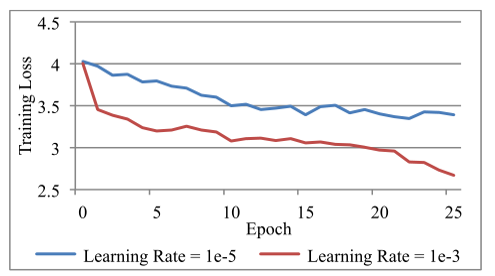
\includegraphics[scale=0.5]{figures/training_loss.png}
%\caption{Loss for various learning rates}
%\label{training_loss}
%\end{figure}

%%%%%%%%%%%%%%%%%%%%%%%%%%%%%%%%%%%%%%%%%%%%%%%%%%%
%
%  New template code for TAMU Theses and Dissertations starting Fall 2012.  
%  For more info about this template or the 
%  TAMU LaTeX User's Group, see http://www.howdy.me/.
%
%  Author: Wendy Lynn Turner 
%	 Version 1.0 
%  Last updated 8/5/2012
%
%%%%%%%%%%%%%%%%%%%%%%%%%%%%%%%%%%%%%%%%%%%%%%%%%%%
%%%%%%%%%%%%%%%%%%%%%%%%%%%%%%%%%%%%%%%%%%%%%%%%%%%%%%%%%%%%%%%%%%%%%%
%%                           SECTION V
%%%%%%%%%%%%%%%%%%%%%%%%%%%%%%%%%%%%%%%%%%%%%%%%%%%%%%%%%%%%%%%%%%%%%


\chapter{\uppercase{Experiments, Results and Analysis}}

In this chapter, I will highlight and analyze the training process and the results for each of the components of our model. 

\section{Dataset Processing}

YOLO needs certain specific files to know how and what to train. As DeepFlow is based on this object detection framework, we must create some configuration files and place them in a configuration folder, named cfg, that will be accessed by our application at the time of training as well as testing. These files are: \textbf{obj.data} which contains the training and text labels in a .txt format,\textbf{obj.names} which containes the different object categories that will be used to identify objects, and \textbf{yolo-obj2.cfg} which contains all the parameters needed for training such as number of batches, number of object categories, number of iterations, learning rate as well as settings for training the network with a gpu or cpu, etc.  The batch size was related to the grid size of the model, with a learning rate of 0.001. In order to reduce the memory footprint and increase computational efficiency of our model, just like in YOLO, all images are first resized to 416 x 416 pixels at both training and testing times. 

\vspace{15mm}
\newpage
Figure \ref{cfg_file} shows how our configuration files looks:

\vspace{15mm}
\begin{figure}[h]
\centering
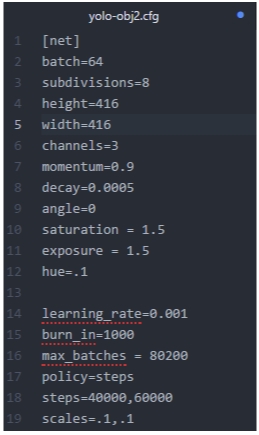
\includegraphics[scale=0.87]{figures/cfg_file.png}
\caption{YOLO Configuration file}
\label{cfg_file}
\end{figure}

\newpage
\section{Dataset Training and Testing Results}
\vspace{5mm}
The entire training log below represents one batch of images, divided according to our subdivisions. We can see the .cfg file shown earlier in Figure \ref{cfg_file} to verify that batch = 64 and subdivision = 8. Looking at the image above, the training iteration has 8 groups of 8 images, reflecting these specific settings.

\vspace{5mm}
\begin{lstlisting}
Loaded: 5.588888 seconds
Region Avg IOU: 0.649881, Class: 0.854394, Obj: 0.476559, No Obj: 0.007302, Avg Recall: 0.737705,  count: 61
Region Avg IOU: 0.671544, Class: 0.959081, Obj: 0.523326, No Obj: 0.006902, Avg Recall: 0.780000,  count: 50
Region Avg IOU: 0.525841, Class: 0.815314, Obj: 0.449031, No Obj: 0.006602, Avg Recall: 0.484375,  count: 64
Region Avg IOU: 0.583596, Class: 0.830763, Obj: 0.377681, No Obj: 0.007916, Avg Recall: 0.629214,  count: 89
Region Avg IOU: 0.651377, Class: 0.908635, Obj: 0.460094, No Obj: 0.008060, Avg Recall: 0.753425,  count: 73
Region Avg IOU: 0.571363, Class: 0.880554, Obj: 0.341659, No Obj: 0.007820, Avg Recall: 0.633663,  count: 101
Region Avg IOU: 0.585424, Class: 0.935552, Obj: 0.358635, No Obj: 0.008192, Avg Recall: 0.644860,  count: 107
Region Avg IOU: 0.599972, Class: 0.832793, Obj: 0.382910, No Obj: 0.009005, Avg Recall: 0.650602,  count: 83
497001: 0.863348, 0.863348 avg, 0.000012 rate, 5.422251 seconds, 107352216 images
\end{lstlisting}

\vspace{5mm}
As we can see in the above listing the last line shows what the batch output is at the moment of training:
\begin{enumerate}
  \item Training batch: 497001.
  \item Total loss:0.863348.
  \item Average loss error: 0.863348 avg, which should be as low as possible in order for us to stopped training the network.
  \item Learning rate that we specified in the configuration file.
  \item Time spent to process the image batch and the total amount of images used during training at this point 5.422251 for 107352216 images.
\end{enumerate}

\vspace{5mm}
The following code snippet illustrates how we log the above training process. By doing this, we are allow the chance to improve our model so that it can be trained in a more efficient way thus delivering better performance in our final application:

\vspace{5mm}
\begin{lstlisting}
def extract_log(log_file,new_log_file,key_word):

    f = open(log_file)
    train_log = open(new_log_file, 'w')

    for line in f:
        if 'Syncing' in line:
            continue
        # Remove the log with zero error
        if 'nan' in line:
            continue
        if key_word in line:
            train_log.write(line)

    f.close()
    train_log.close()

extract_log('coco_train_log.txt','coco_train_log_loss.txt','images')
extract_log ( ' coco_train_log.txt ' , ' coco_train_log_iou.txt ' , ' IOU ' )
\end{lstlisting}

\vspace{5mm}
In our re-implementation of DeepFlow, a YOLO object detection and tracking system, we have initially used PASCAL-VOC for faster training and testing of our system. Nonetheless, this dataset has a limitation for our application since it only offers a limited number of categories, 20 classes and our mindset is for our application to be able to identify and track at least 80 to 100 object categories. Therefore, we decided for our final application to use COCO DATASET which is a large-scale object detection, segmentation, and captioning dataset with several advantages for research in the field of computer vision. The dataset offers 330k+ images, recognition in context, 80 object categories, and many other features that we will use for our advantage to train and test our network.

\newpage
When using PASCAL-VOC which is a lighter dataset that can be easily trained and test in a few hours on a laptop since it needs less training steps than other datasets such as COCO,PASCAL-VOC comes almost pre-trained from ImageNet. Therefore, the training scope boils down only to adding specific layers for new recognition tasks by using the previous learned knowledge.

Figure \ref{test_graph} shows the statistics of our training using PASCAL-VOC:
\begin{figure}[h]
\centering
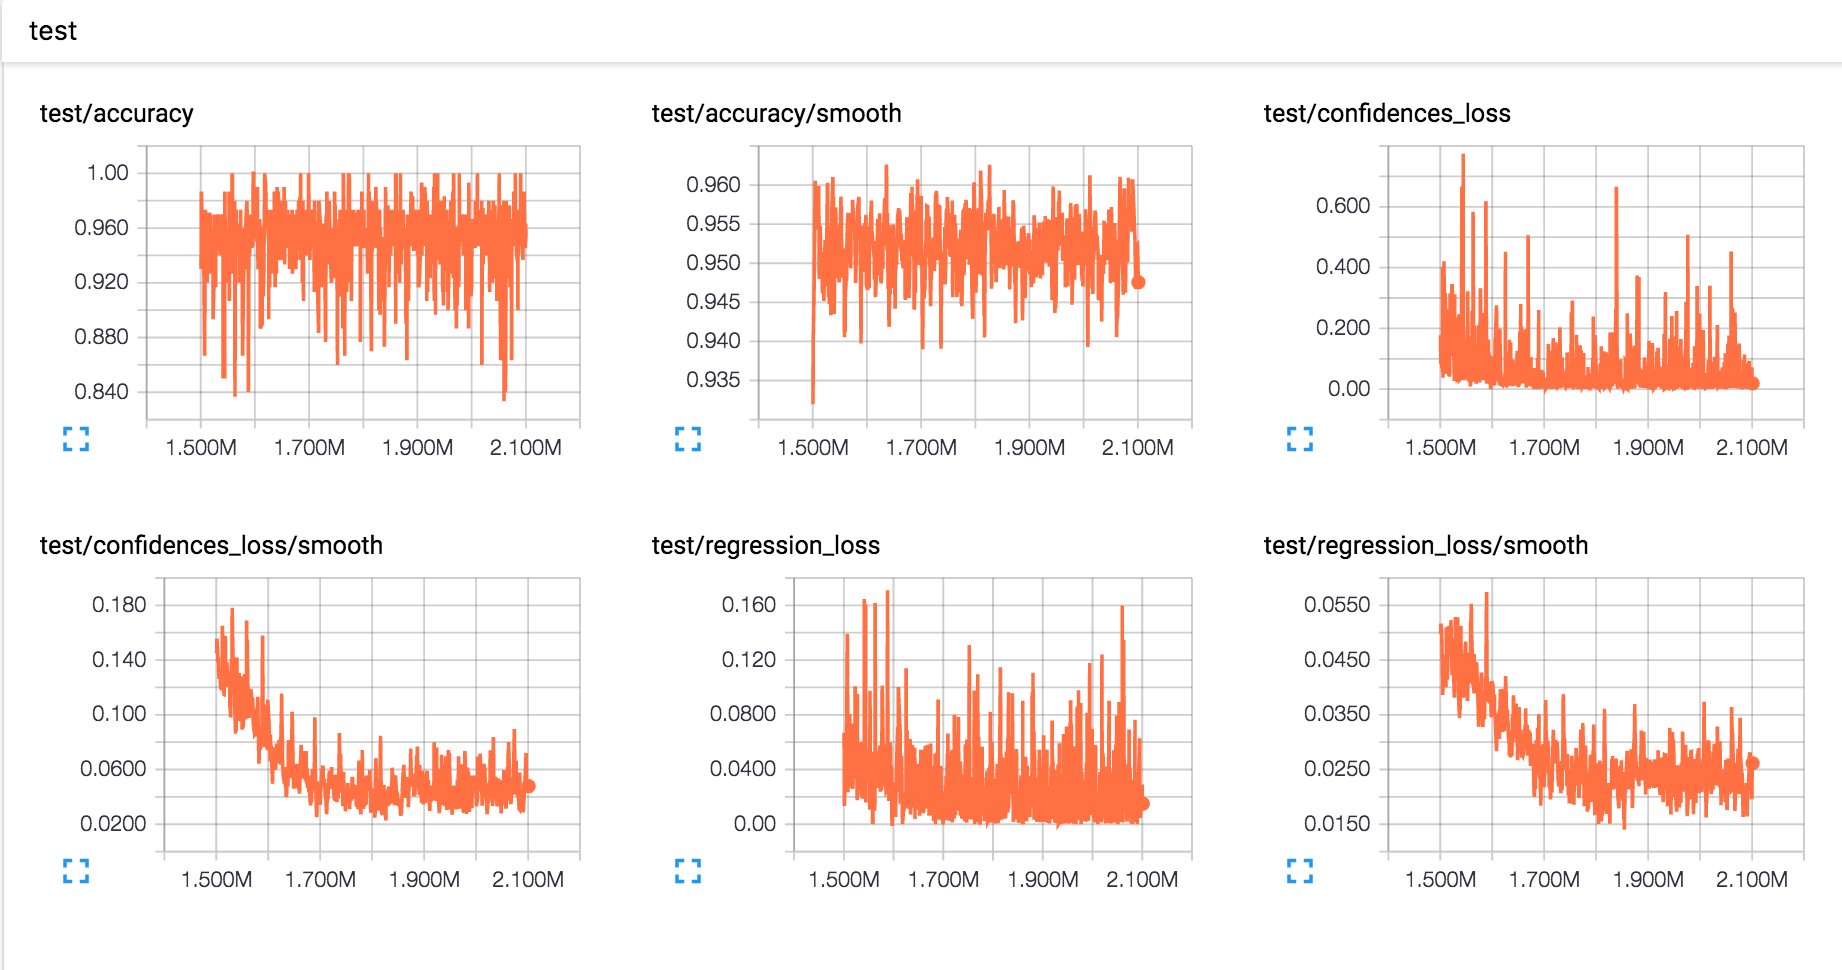
\includegraphics[scale=0.2]{figures/test_graph.png}
\caption{PASCAL-VOC Training Graph}
\label{test_graph}
\end{figure}

As we can see in training accuracy and cross-entropy cost function graphs both functions flatten due our model only focusing on 20 - 30  classes of a few  objects it already knows. Figures \ref{accuracy_crossentropy} below highlights that the graph learns well.

\begin{figure}
\centering
\begin{subfigure}{.5\textwidth}
  \centering
  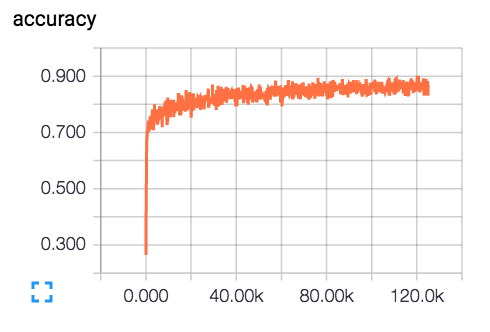
\includegraphics[width=.8\linewidth]{figures/graph_accuracy.png}
  \caption{Training Accuracy}
  \label{fig:sub1}
\end{subfigure}%
\begin{subfigure}{.5\textwidth}
  \centering
  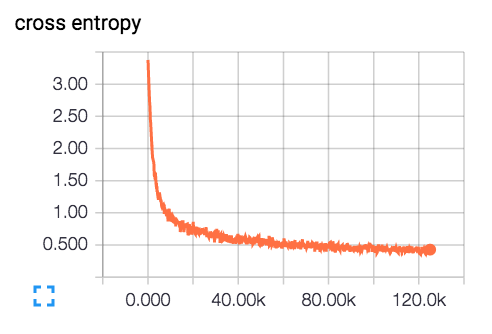
\includegraphics[width=.8\linewidth]{figures/cross_entropy.png}
  \caption{Cross Entropy Cost Function}
  \label{fig:sub2}
\end{subfigure}
\caption{Traing Accuracy and Cross Entropy Cost Function}
\label{fig:accuracy_crossentropy}
\end{figure}

\newpage
for our final application in order to achieve an acceptable performance comparable to YOLO using a larger dataset like COCO, we had to train our network for a couple of days. Initially, we got not so good results due to the fact that our implementation performance was too slow to learn. Learning was inaccurate leading to bad performance while using both GPU and CPU. 

In order to improve performance, we decided to use Tensorbox to help in the training process. As we can see from the graphs in figure \ref{training_graph_tf}, all functions flatten with sparse results and peaks. This happens because of generalization of the model which is not learning different masks for each object category which reduces our accuracy while training.


\begin{figure}[h]
\centering
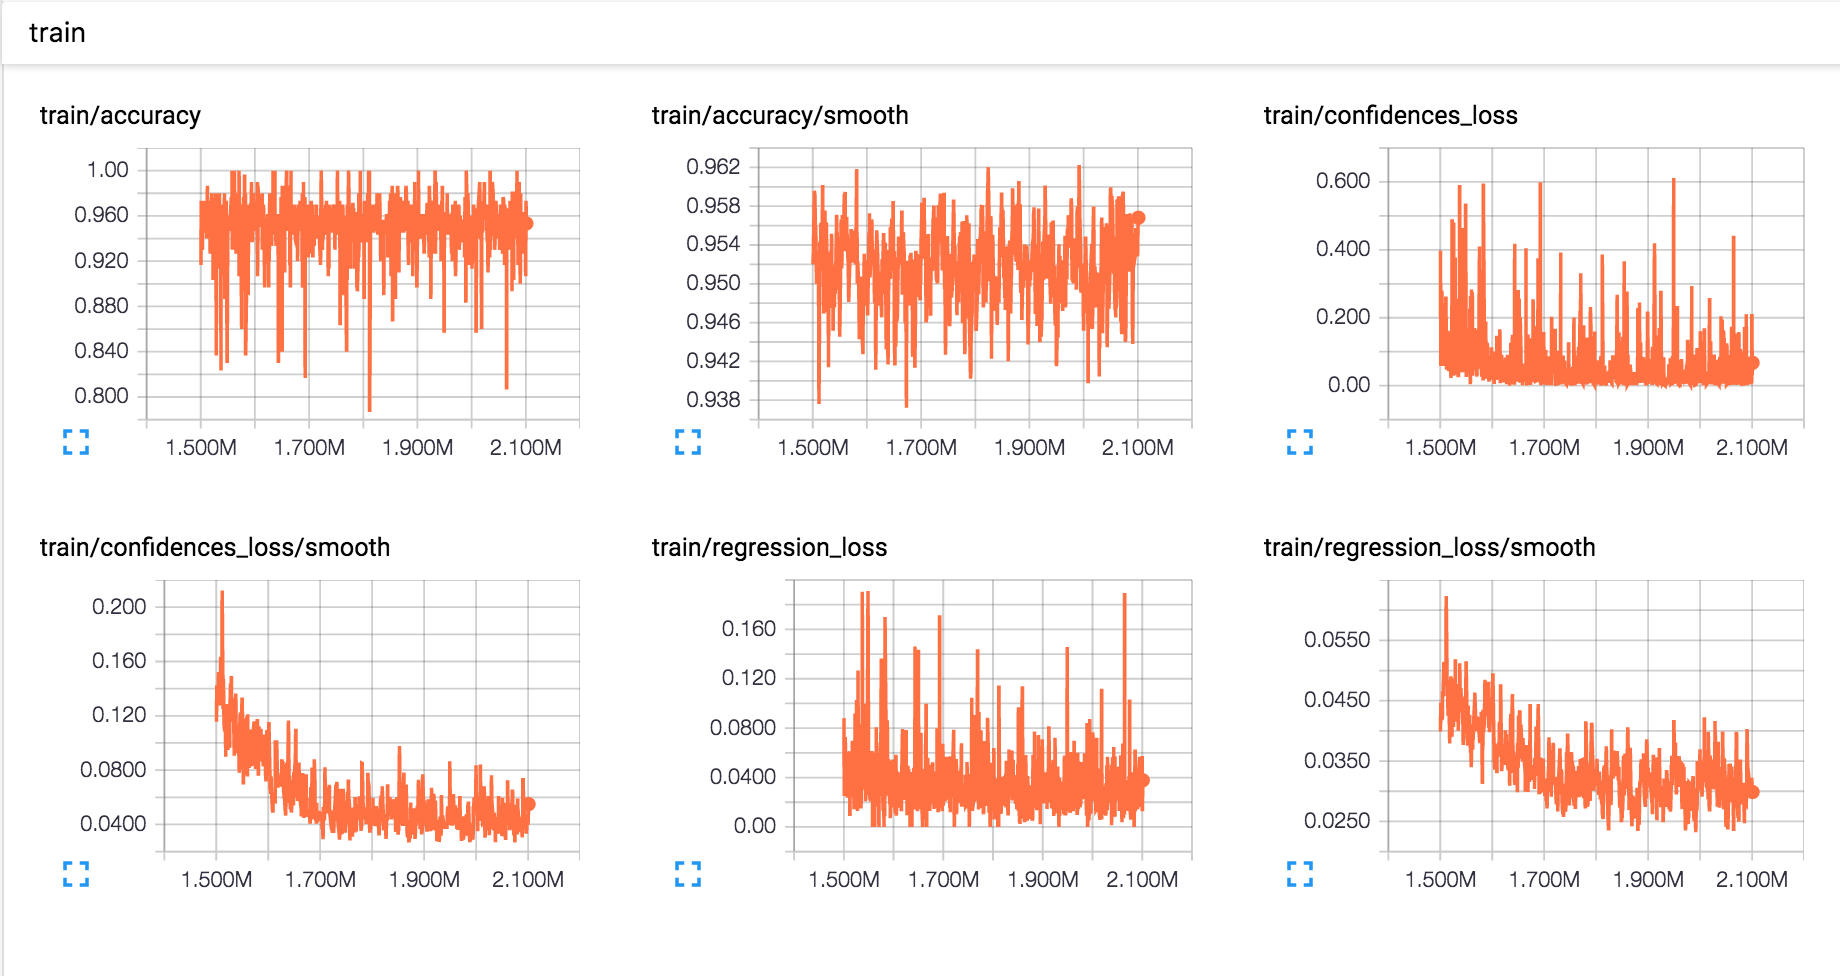
\includegraphics[scale=0.3]{figures/training_graph_tf.png}
\caption{DeepFlow Configuration file}
\label{training_graph_tf}
\end{figure}

\newpage
As figure \ref{weights_norm} shows that the weights of our model, after some iterations, flatten what let us know that the model was not learning any more.

\begin{figure}[h]
\centering
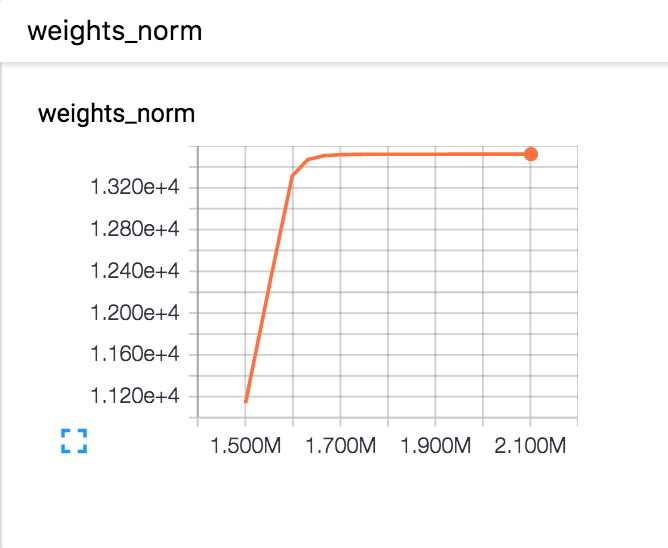
\includegraphics[scale=0.3]{figures/weights_norm.png}
\caption{Weights from first training results}
\label{weights_norm}
\end{figure}

Below, we show some screenshots of our first tests of the exported model where we have some degree of  inaccuracy when detecting objects:

\begin{figure}
\centering
\begin{subfigure}{.5\textwidth}
  \centering
  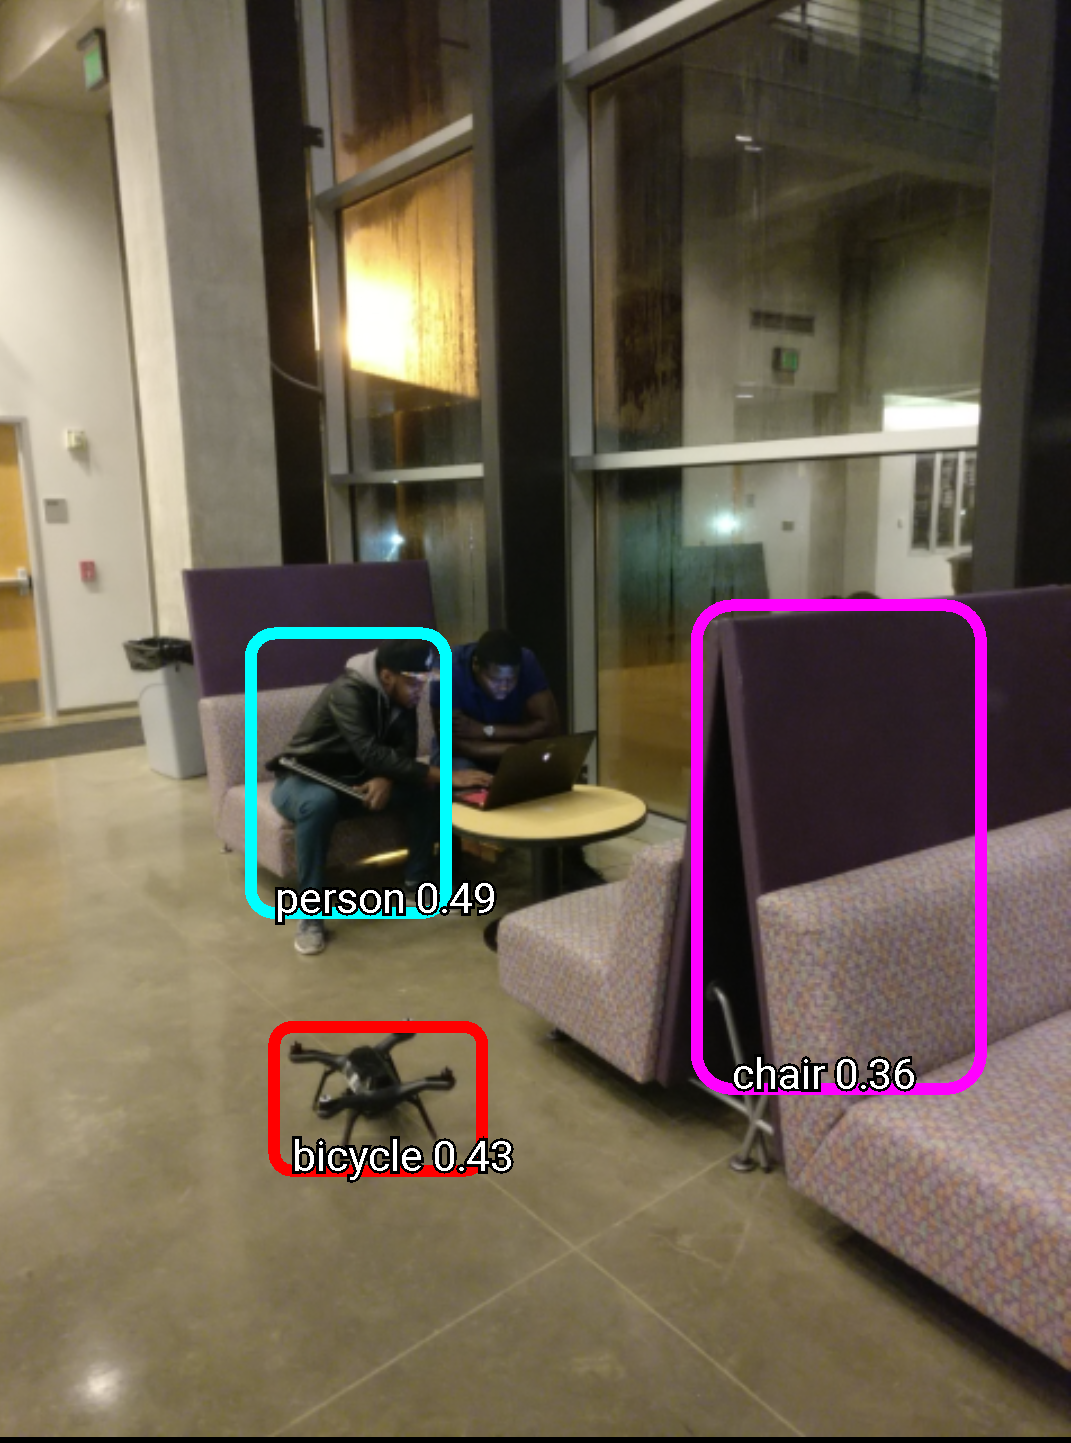
\includegraphics[width=.4\linewidth]{figures/test_2.png}
  \caption{Detection Accuracy Test}
  \label{fig:sub1}
\end{subfigure}%
\begin{subfigure}{.5\textwidth}
  \centering
  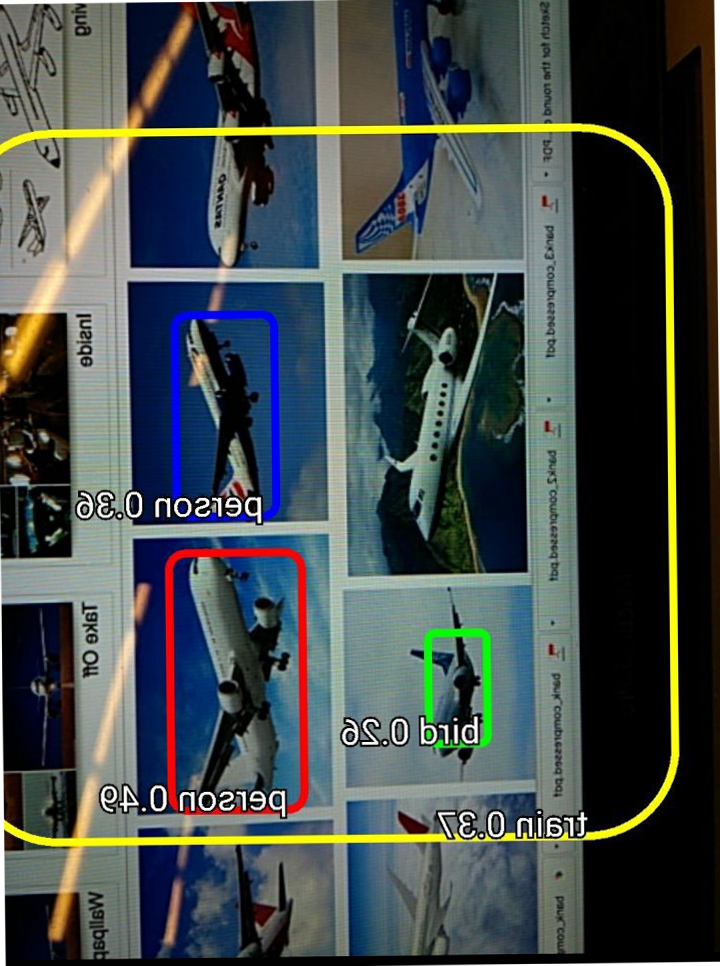
\includegraphics[width=.4\linewidth]{figures/test_7.png}
  \caption{Detection Accuracy Test}
  \label{fig:sub2}
\end{subfigure}
\caption{DeepFlow Object Detection Accuracy Test}
\label{fig:accuracy_test}
\end{figure}

\newpage
Due to  bad results obtained in the first days of training, we upgraded our network to improve training and thus, obtaining better learning rates as well as better detection and tracking results.

The code implementation for training below shows our modified network and the graph output:

\vspace{3mm}
\begin{lstlisting}
import os
import argparse
import configparser
import importlib
import shutil
import time
import inspect
import multiprocessing
import tensorflow as tf
import tensorflow.contrib.slim as slim
import utils.data


def summary_scalar(config):
    try:
        reduce = eval(config.get('summary', 'scalar_reduce'))
        for t in utils.match_tensor(config.get('summary', 'scalar')):
            name = t.op.name
            if len(t.get_shape()) > 0:
                t = reduce(t)
                tf.logging.warn(name + ' is not a scalar tensor, reducing by ' + reduce.__name__)
            tf.summary.scalar(name, t)
    except (configparser.NoSectionError, configparser.NoOptionError):
        tf.logging.warn(inspect.stack()[0][3] + ' disabled')


def summary_image(config):
    try:
        for t in utils.match_tensor(config.get('summary', 'image')):
            name = t.op.name
            channels = t.get_shape()[-1].value
            if channels not in (1, 3, 4):
                t = tf.expand_dims(tf.reduce_sum(t, -1), -1)
            tf.summary.image(name, t, config.getint('summary', 'image_max'))
    except (configparser.NoSectionError, configparser.NoOptionError):
        tf.logging.warn(inspect.stack()[0][3] + ' disabled')


def summary_histogram(config):
    try:
        for t in utils.match_tensor(config.get('summary', 'histogram')):
            tf.summary.histogram(t.op.name, t)
    except (configparser.NoSectionError, configparser.NoOptionError):
        tf.logging.warn(inspect.stack()[0][3] + ' disabled')


def summary(config):
    summary_scalar(config)
    summary_image(config)
    summary_histogram(config)


def get_optimizer(config, name):
    section = 'optimizer_' + name
    return {
        'adam': lambda learning_rate: tf.train.AdamOptimizer(learning_rate, config.getfloat(section, 'beta1'), config.getfloat(section, 'beta2'), config.getfloat(section, 'epsilon')),
        'adadelta': lambda learning_rate: tf.train.AdadeltaOptimizer(learning_rate, config.getfloat(section, 'rho'), config.getfloat(section, 'epsilon')),
        'adagrad': lambda learning_rate: tf.train.AdagradOptimizer(learning_rate, config.getfloat(section, 'initial_accumulator_value')),
        'momentum': lambda learning_rate: tf.train.MomentumOptimizer(learning_rate, config.getfloat(section, 'momentum')),
        'rmsprop': lambda learning_rate: tf.train.RMSPropOptimizer(learning_rate, config.getfloat(section, 'decay'), config.getfloat(section, 'momentum'), config.getfloat(section, 'epsilon')),
        'ftrl': lambda learning_rate: tf.train.FtrlOptimizer(learning_rate, config.getfloat(section, 'learning_rate_power'), config.getfloat(section, 'initial_accumulator_value'), config.getfloat(section, 'l1_regularization_strength'), config.getfloat(section, 'l2_regularization_strength')),
        'gd': lambda learning_rate: tf.train.GradientDescentOptimizer(learning_rate),
    }[name]


def main():
    model = config.get('config', 'model')
    logdir = utils.get_logdir(config)
    if args.delete:
        tf.logging.warn('delete logging directory: ' + logdir)
        shutil.rmtree(logdir, ignore_errors=True)
    cachedir = utils.get_cachedir(config)
    with open(os.path.join(cachedir, 'names'), 'r') as f:
        names = [line.strip() for line in f]
    width = config.getint(model, 'width')
    height = config.getint(model, 'height')
    cell_width, cell_height = utils.calc_cell_width_height(config, width, height)
    tf.logging.warn('(width, height)=(%d, %d), (cell_width, cell_height)=(%d, %d)' % (width, height, cell_width, cell_height))
    yolo = importlib.import_module('model.' + model)
    paths = [os.path.join(cachedir, profile + '.tfrecord') for profile in args.profile]
    num_examples = sum(sum(1 for _ in tf.python_io.tf_record_iterator(path)) for path in paths)
    tf.logging.warn('num_examples=%d' % num_examples)
    with tf.name_scope('batch'):
        image_rgb, labels = utils.data.load_image_labels(paths, len(names), width, height, cell_width, cell_height, config)
        with tf.name_scope('per_image_standardization'):
            image_std = tf.image.per_image_standardization(image_rgb)
        batch = tf.train.shuffle_batch((image_std,) + labels, batch_size=args.batch_size,
            capacity=config.getint('queue', 'capacity'), min_after_dequeue=config.getint('queue', 'min_after_dequeue'),
            num_threads=multiprocessing.cpu_count()
        )
    global_step = tf.contrib.framework.get_or_create_global_step()
    builder = yolo.Builder(args, config)
    builder(batch[0], training=True)
    with tf.name_scope('total_loss') as name:
        builder.create_objectives(batch[1:])
        total_loss = tf.losses.get_total_loss(name=name)
    variables_to_restore = slim.get_variables_to_restore(exclude=args.exclude)
    with tf.name_scope('optimizer'):
        try:
            decay_steps = config.getint('exponential_decay', 'decay_steps')
            decay_rate = config.getfloat('exponential_decay', 'decay_rate')
            staircase = config.getboolean('exponential_decay', 'staircase')
            learning_rate = tf.train.exponential_decay(args.learning_rate, global_step, decay_steps, decay_rate, staircase=staircase)
            tf.logging.warn('using a learning rate start from %f with exponential decay (decay_steps=%d, decay_rate=%f, staircase=%d)' % (args.learning_rate, decay_steps, decay_rate, staircase))
        except (configparser.NoSectionError, configparser.NoOptionError):
            learning_rate = args.learning_rate
            tf.logging.warn('using a staionary learning rate %f' % args.learning_rate)
        optimizer = get_optimizer(config, args.optimizer)(learning_rate)
        tf.logging.warn('optimizer=' + args.optimizer)
        train_op = slim.learning.create_train_op(total_loss, optimizer, global_step,
            clip_gradient_norm=args.gradient_clip, summarize_gradients=config.getboolean('summary', 'gradients'),
        )
    if args.transfer:
        path = os.path.expanduser(os.path.expandvars(args.transfer))
        tf.logging.warn('transferring from ' + path)
        init_assign_op, init_feed_dict = slim.assign_from_checkpoint(path, variables_to_restore)
        def init_fn(sess):
            sess.run(init_assign_op, init_feed_dict)
            tf.logging.warn('transferring from global_step=%d, learning_rate=%f' % sess.run((global_step, learning_rate)))
    else:
        init_fn = lambda sess: tf.logging.warn('global_step=%d, learning_rate=%f' % sess.run((global_step, learning_rate)))
    summary(config)
    tf.logging.warn('tensorboard --logdir ' + logdir)
    slim.learning.train(train_op, logdir, master=args.master, is_chief=(args.task == 0),
        global_step=global_step, number_of_steps=args.steps, init_fn=init_fn,
        summary_writer=tf.summary.FileWriter(os.path.join(logdir, args.logname)),
        save_summaries_secs=args.summary_secs, save_interval_secs=args.save_secs
    )


def make_args():
    parser = argparse.ArgumentParser()
    parser.add_argument('-c', '--config', nargs='+', default=['config.ini'], help='config file')
    parser.add_argument('-t', '--transfer', help='transferring model from a .ckpt file')
    parser.add_argument('-e', '--exclude', nargs='+', help='exclude variables while transferring')
    parser.add_argument('-p', '--profile', nargs='+', default=['train', 'val'])
    parser.add_argument('-s', '--steps', type=int, default=None, help='max number of steps')
    parser.add_argument('-d', '--delete', action='store_true', help='delete logdir')
    parser.add_argument('-b', '--batch_size', default=8, type=int, help='batch size')
    parser.add_argument('-o', '--optimizer', default='adam')
    parser.add_argument('-n', '--logname', default=time.strftime('%Y-%m-%d_%H-%M-%S'), help='the name for TensorBoard')
    parser.add_argument('-g', '--gradient_clip', default=0, type=float, help='gradient clip')
    parser.add_argument('-lr', '--learning_rate', default=1e-6, type=float, help='learning rate')
    parser.add_argument('--seed', type=int, default=None)
    parser.add_argument('--summary_secs', default=30, type=int, help='seconds to save summaries')
    parser.add_argument('--save_secs', default=600, type=int, help='seconds to save model')
    parser.add_argument('--level', help='logging level')
    parser.add_argument('--master', default='', help='master address')
    parser.add_argument('--task', type=int, default=0, help='task ID')
    return parser.parse_args()

if __name__ == '__main__':
    args = make_args()
    config = configparser.ConfigParser()
    utils.load_config(config, args.config)
    if args.level:
        tf.logging.set_verbosity(args.level.upper())
    main()
\end{lstlisting}

%\begin{lstlisting}
%import pandas as pd
%import numpy as np
%import matplotlib.pyplot as plt
%
%lines =1878760
%result = pd.read_csv('/home/ludwi/coco_YOLO/coco_train_log_new.txt', skiprows=[x for x in range(lines) if ((x%10!=9) |(x<1000))] ,error_bad_lines=False, names=['loss', 'avg', 'rate', 'seconds', 'images'])
%result.head()
%
%result['loss']=result['loss'].str.split(' ').str.get(1)
%result['avg']=result['avg'].str.split(' ').str.get(1)
%result['rate']=result['rate'].str.split(' ').str.get(1)
%result['seconds']=result['seconds'].str.split(' ').str.get(1)
%result['images']=result['images'].str.split(' ').str.get(1)
%result.head()
%result.tail()
%
%#print(result.head())
%# print(result.tail())
%# print(result.dtypes)
%
%print(result['loss'])
%print(result['avg'])
%print(result['rate'])
%print(result['seconds'])
%print(result['images'])
%
%result['loss']=pd.to_numeric(result['loss'])
%result['avg']=pd.to_numeric(result['avg'])
%result['rate']=pd.to_numeric(result['rate'])
%result['seconds']=pd.to_numeric(result['seconds'])
%result['images']=pd.to_numeric(result['images'])
%result.dtypes
%
%
%fig = plt.figure()
%ax = fig.add_subplot(1, 1, 1)
%ax.plot(result['avg'].values,label='avg_loss')
%#ax.plot(result['loss'].values,label='loss')
%ax.legend(loc='best')
%ax.set_title('The loss curves')
%ax.set_xlabel('batches')
%fig.savefig('avg_loss')
%#fig.savefig('loss')
%\end{lstlisting}

%\begin{figure}[h]
%\centering
%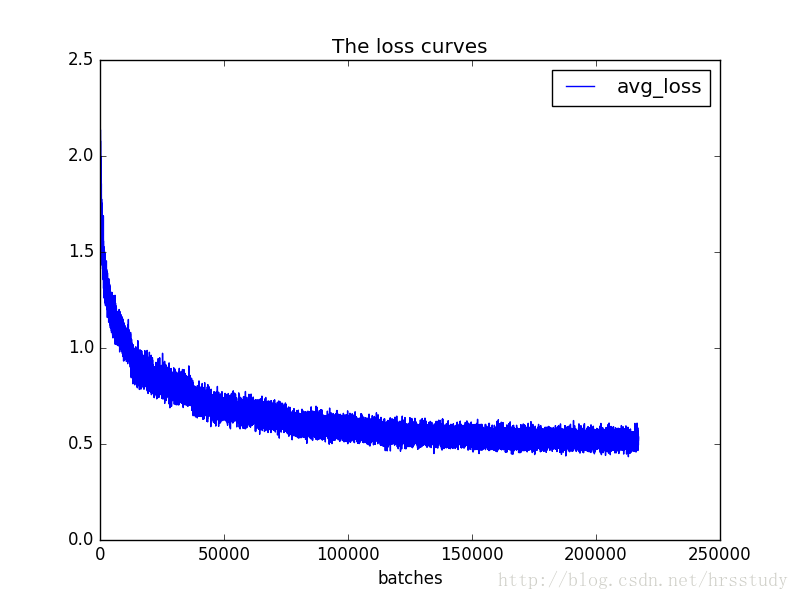
\includegraphics[scale=0.6]{figures/curve_loss.png}
%\caption{DeepFlow Training accuracy}
%\label{deepFlow_graph}
%\end{figure}

\newpage
\begin{figure}
\centering
\begin{subfigure}{.5\textwidth}
  \centering
  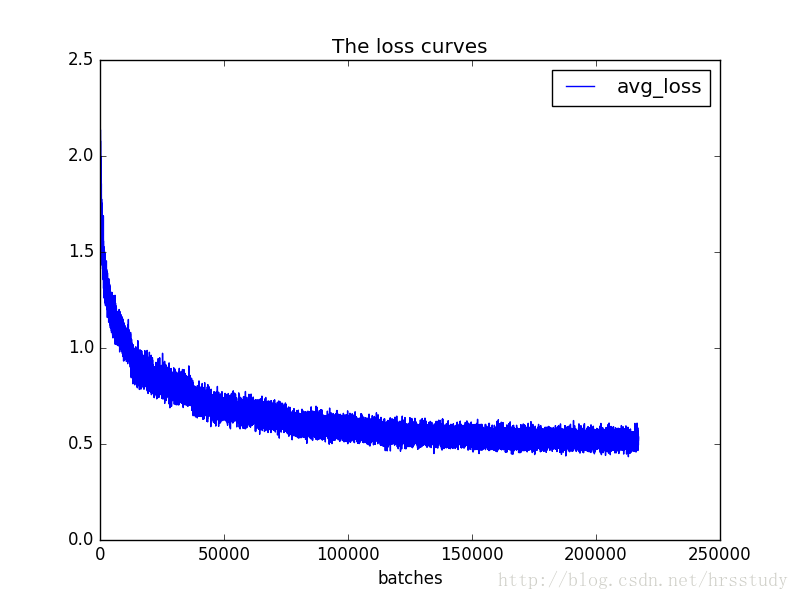
\includegraphics[width=.5\linewidth]{figures/curve_loss.png}
  \caption{DeepFlow Training accuracy}
  \label{fig:deepFlow_graph}
\end{subfigure}%
\begin{subfigure}{.5\textwidth}
  \centering
  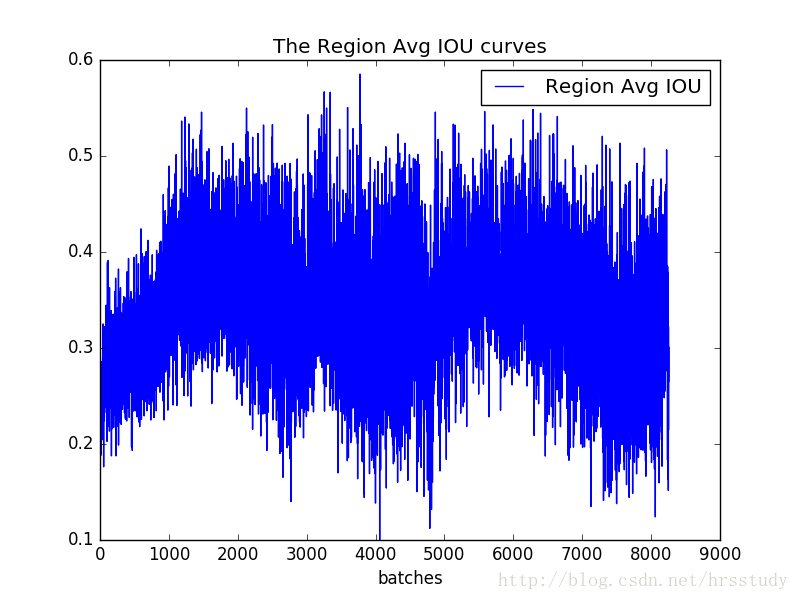
\includegraphics[width=.5\linewidth]{figures/avg_IOU.png}
  \caption{DeepFlow IOU}
  \label{fig:DeepFlow_IOU}
\end{subfigure}
\caption{DeepFlow Object Detection Accuracy Test}
\label{fig:deep_accuracy}
\end{figure}

From the loss curve  in figure \ref{deep_accuracy} \ref{deepFlow_graph}, it can be seen that while training our model again the decline rate of the loss function is very slow, almost no decline, when it reaches a certain number of iterations. Further analysis of the log and .cfg files reveals that the custom learning rate change strategy, we set, is reduced by ten times over 100,000 iterations resulting in a decrease in loss rate. Therefore, we perform some modifications on the learning rate change strategy in cfg to get better results.

To further improve DeepFlow, we had to also optimize the IOU (figure \ref{IOU_fig}) obtained during or training. IOU is a great way to determine how accurate our model is able to perform detection of certain objects.If we get a 100\% IOU, we would have a perfect detection system: a perfect overlap of our bounding box and the target. 

\begin{figure}[ht]
\centering
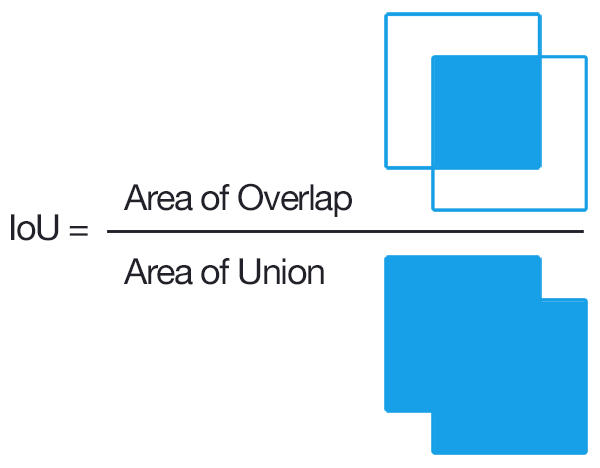
\includegraphics[scale=0.2]{figures/IOU.png}
\caption{DeepFlow IOU}
\label{IOU_fig}
\end{figure}

The test image above shows how really the model is learning, where it becomes easier to detect objects in monochrome backgrounds (like airplanes into the figure of the
whole process), but training to detect generalized object, where this condition is not satisfied, gives us a lower accuracy, more if overlapped object are present.

\begin{figure}
\centering
\begin{subfigure}{.4\textwidth}
  \centering
  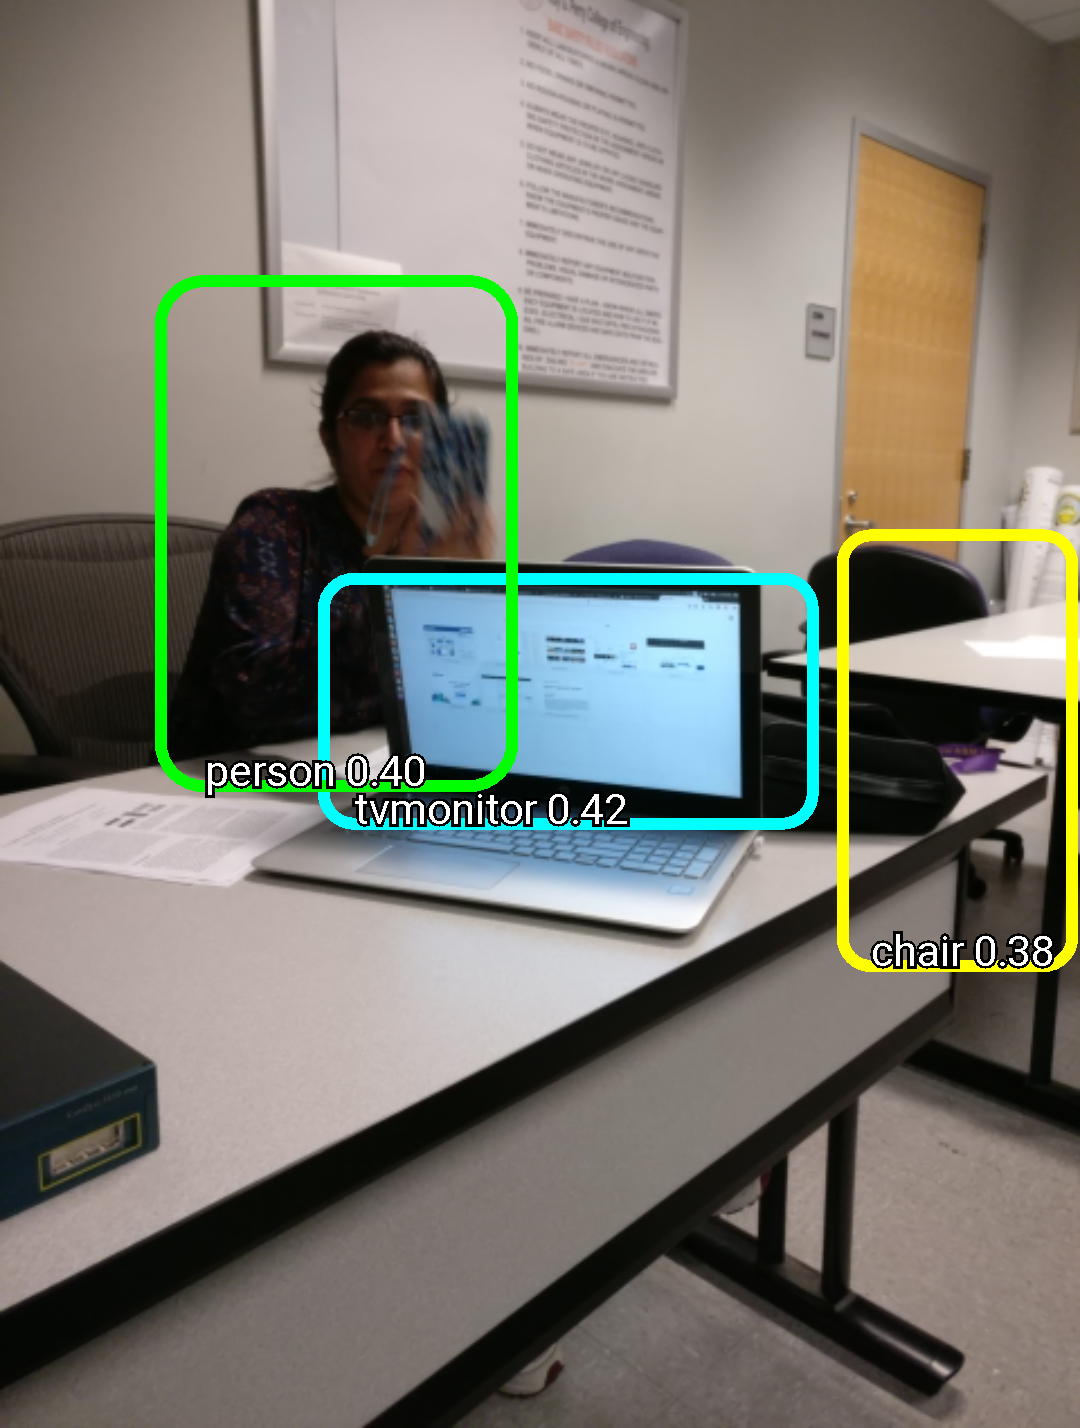
\includegraphics[width=.5\linewidth]{figures/test_4.png}
  \caption{DeepFlow Test}
  \label{fig:deepFlow_graph}
\end{subfigure}
\begin{subfigure}{.4\textwidth}
  \centering
  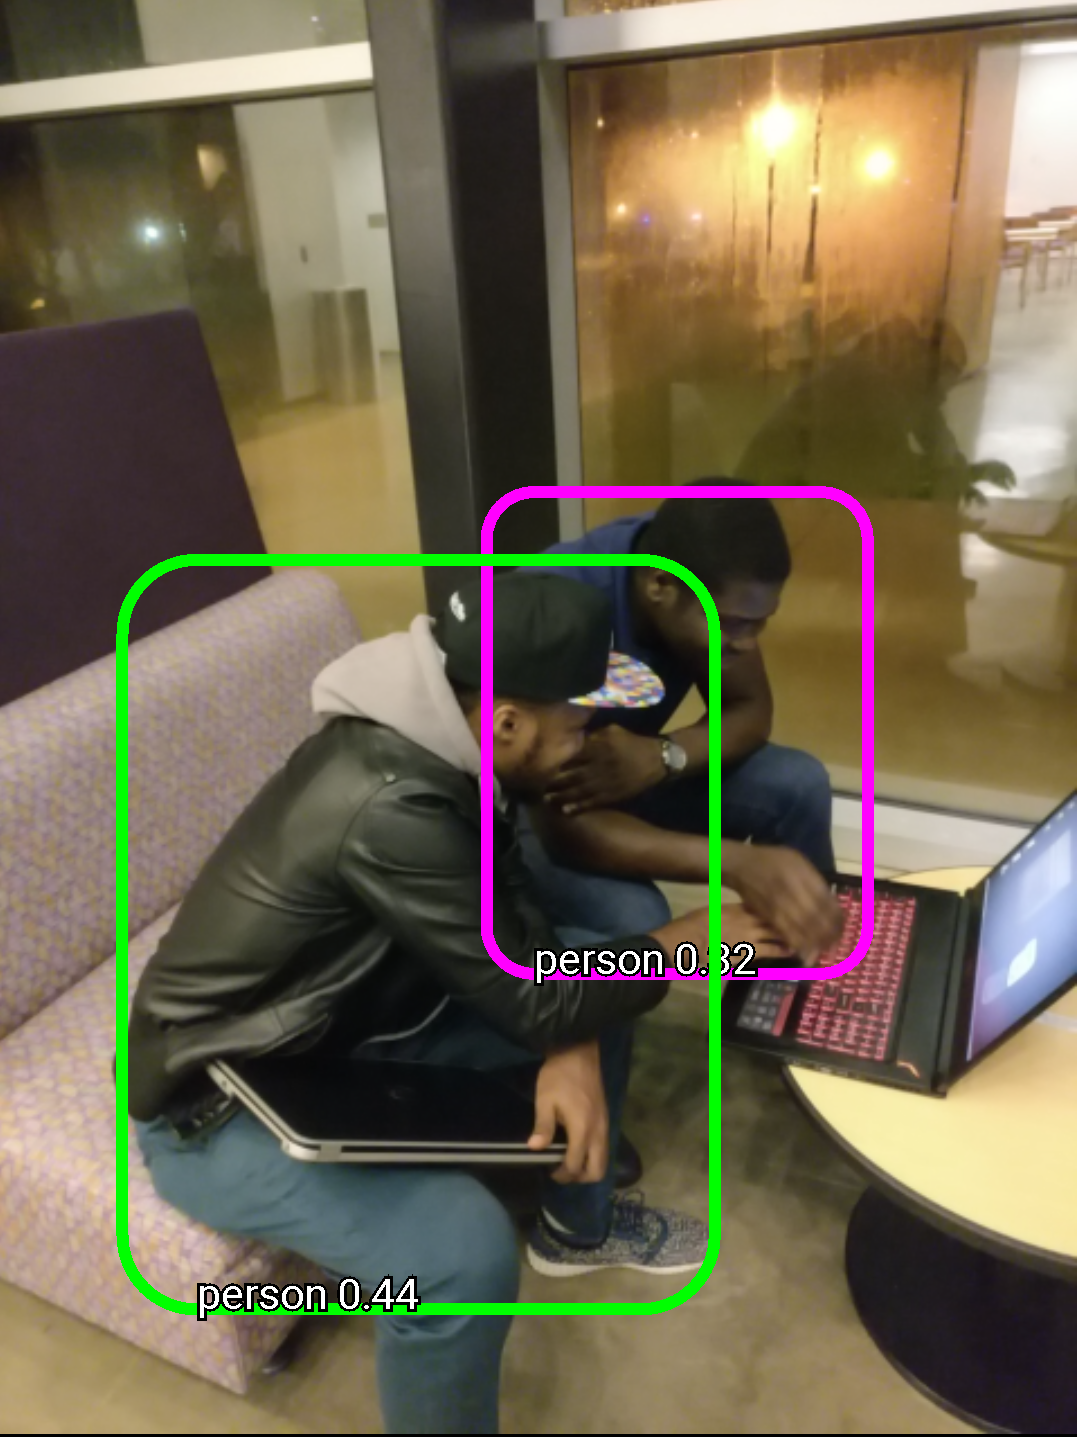
\includegraphics[width=.5\linewidth]{figures/test_1.png}
  \caption{DeepFlow IOU}
  \label{fig:DeepFlow_IOU}
\end{subfigure}
\begin{subfigure}{.4\textwidth}
  \centering
  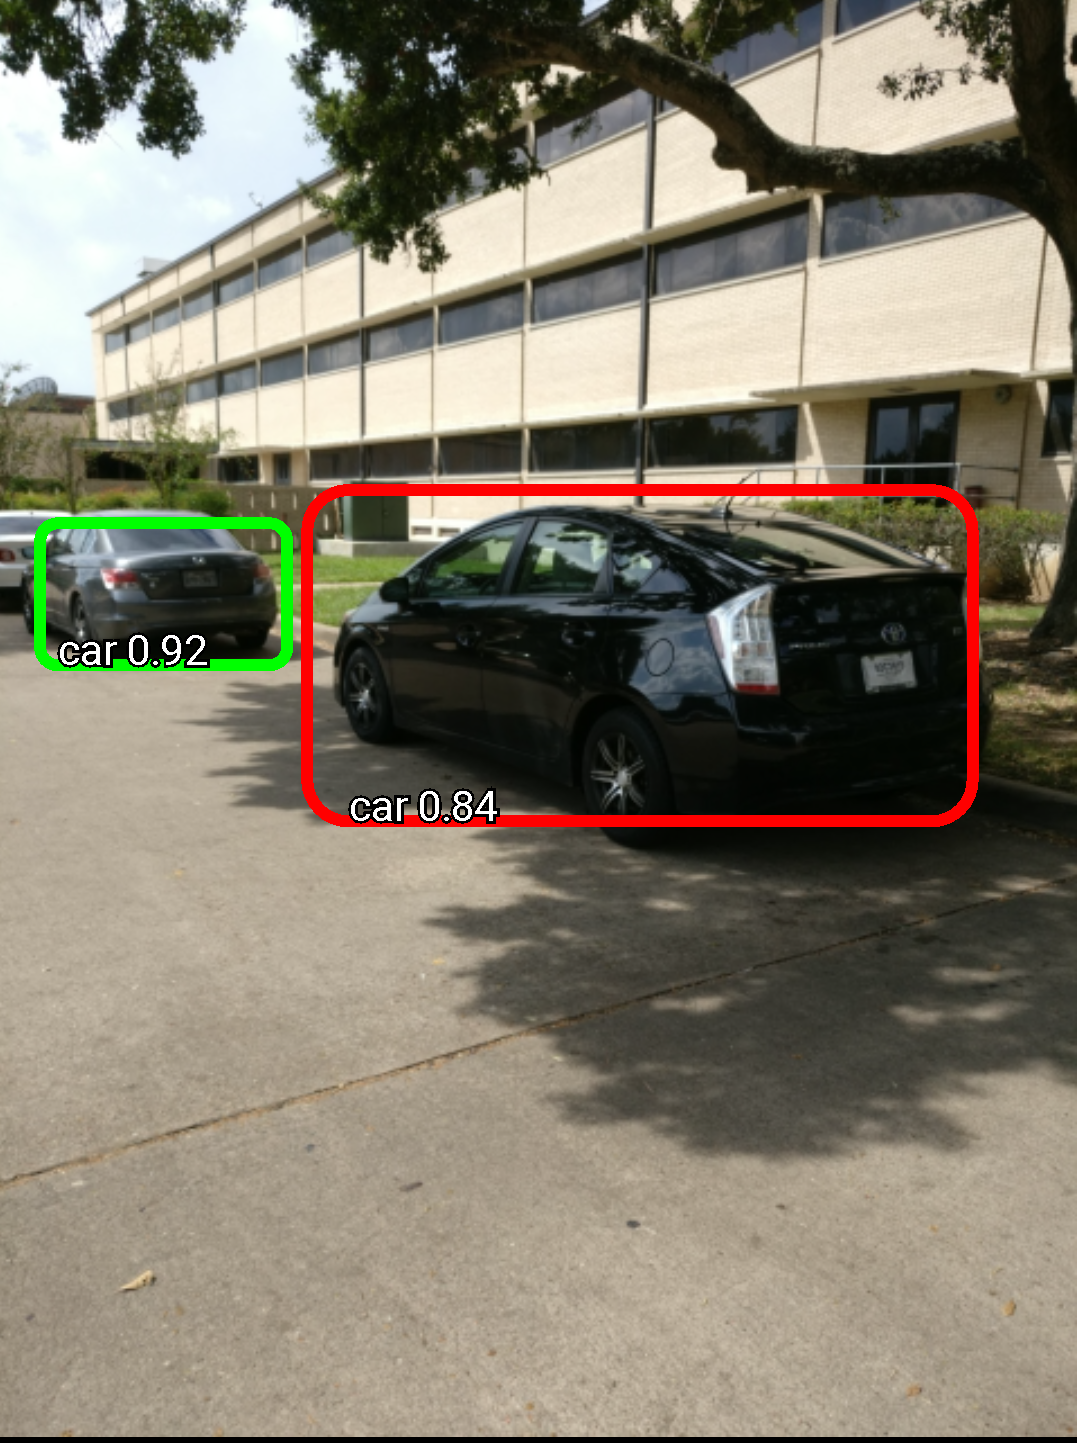
\includegraphics[width=.5\linewidth]{figures/test_3.png}
  \caption{DeepFlow  Test}
  \label{fig:deepFlow_graph}
\end{subfigure}
\begin{subfigure}{.4\textwidth}
  \centering
  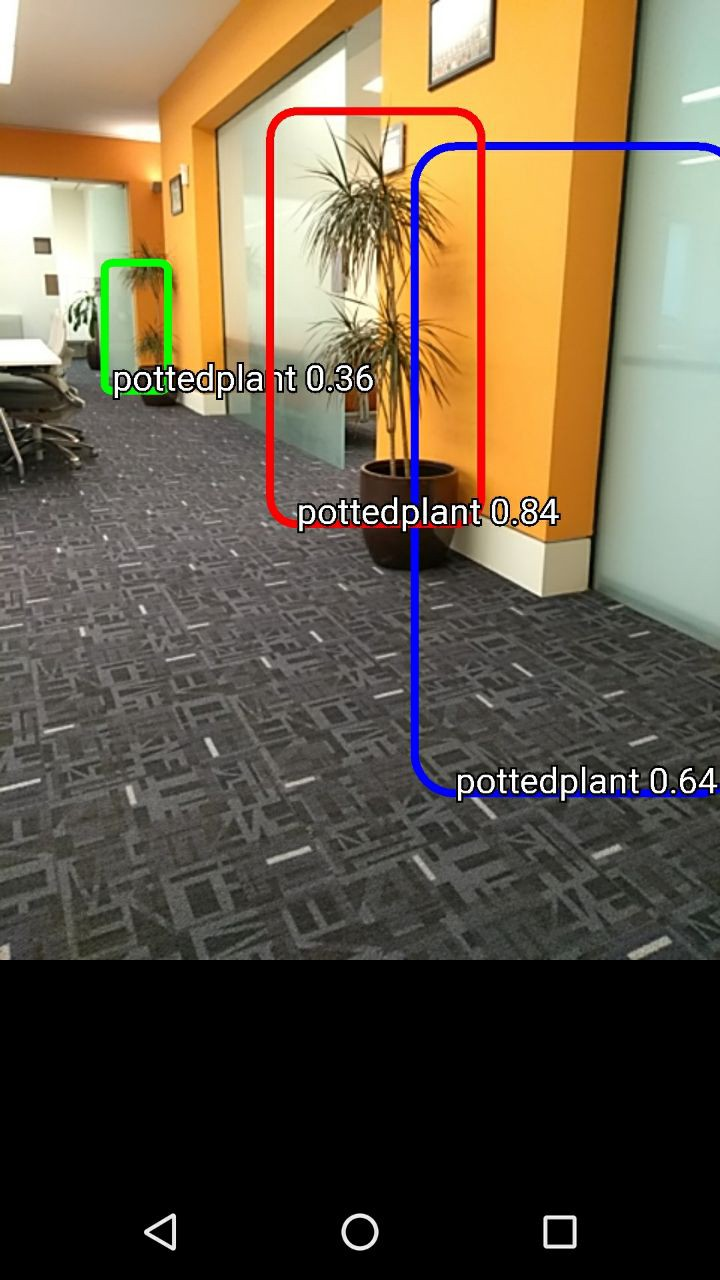
\includegraphics[width=.5\linewidth]{figures/test_6.jpeg}
  \caption{DeepFlow IOU}
  \label{fig:DeepFlow_IOU}
\end{subfigure}
\caption{DeepFlow  Test}
\label{fig:deep_accuracy}
\end{figure}

%\begin{figure}
%\centering
%\begin{subfigure}{.4\textwidth}
%  \centering
%  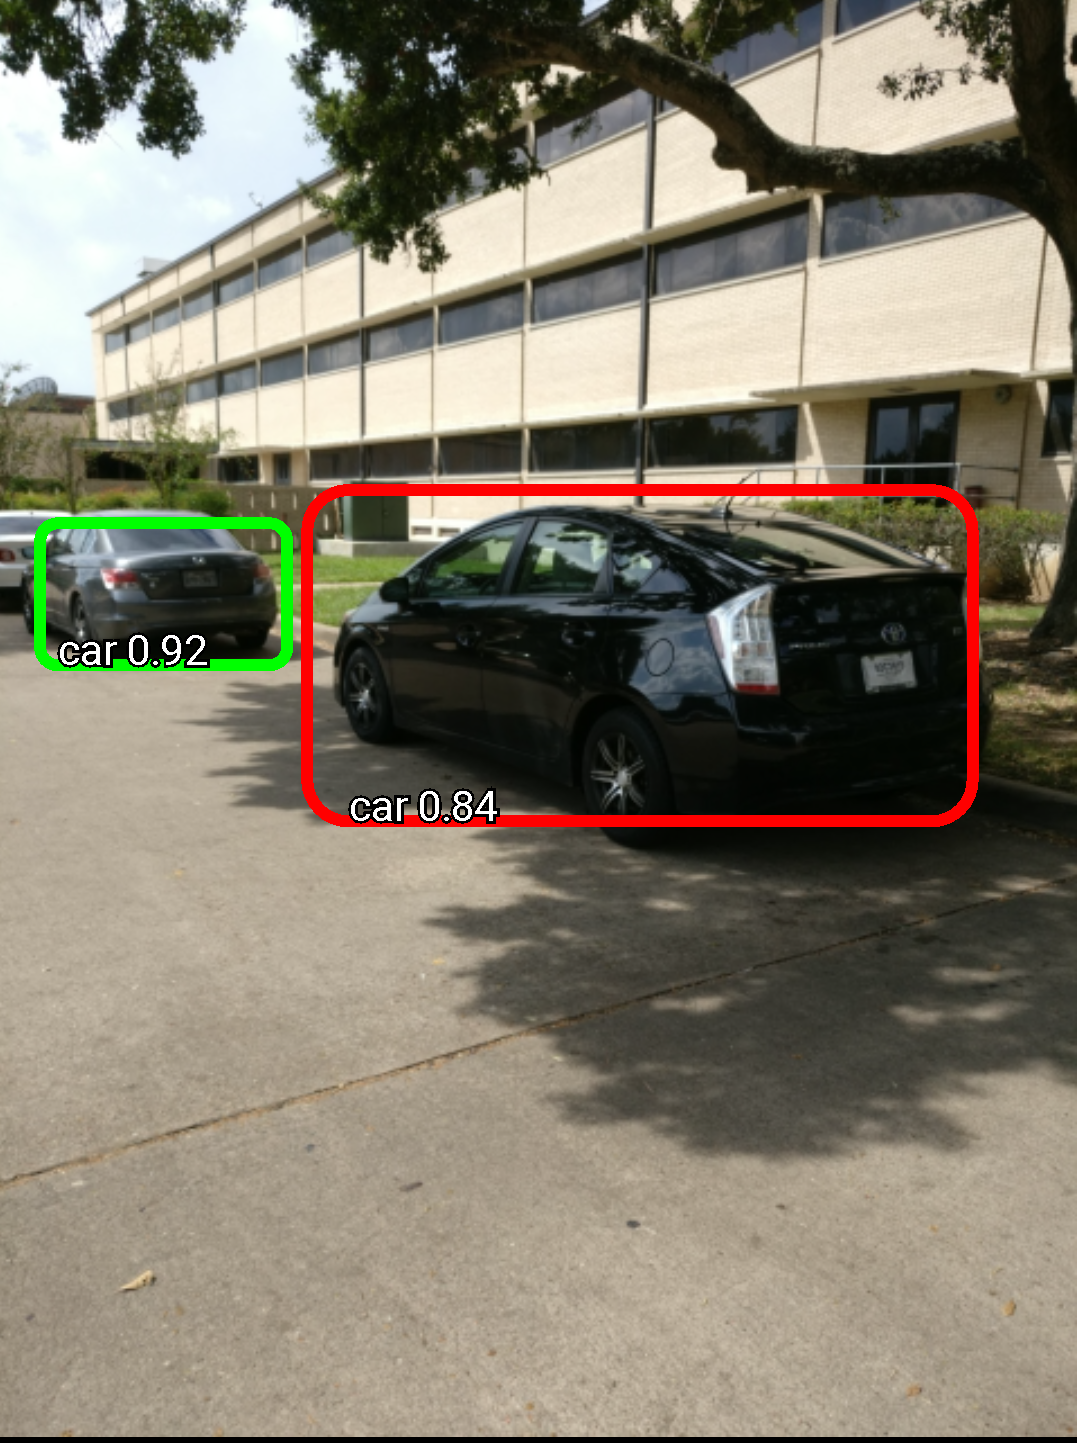
\includegraphics[width=.5\linewidth]{figures/test_3.png}
%  \caption{DeepFlow  Test}
%  \label{fig:deepFlow_graph}
%\end{subfigure}%
%\begin{subfigure}{.4\textwidth}
%  \centering
%  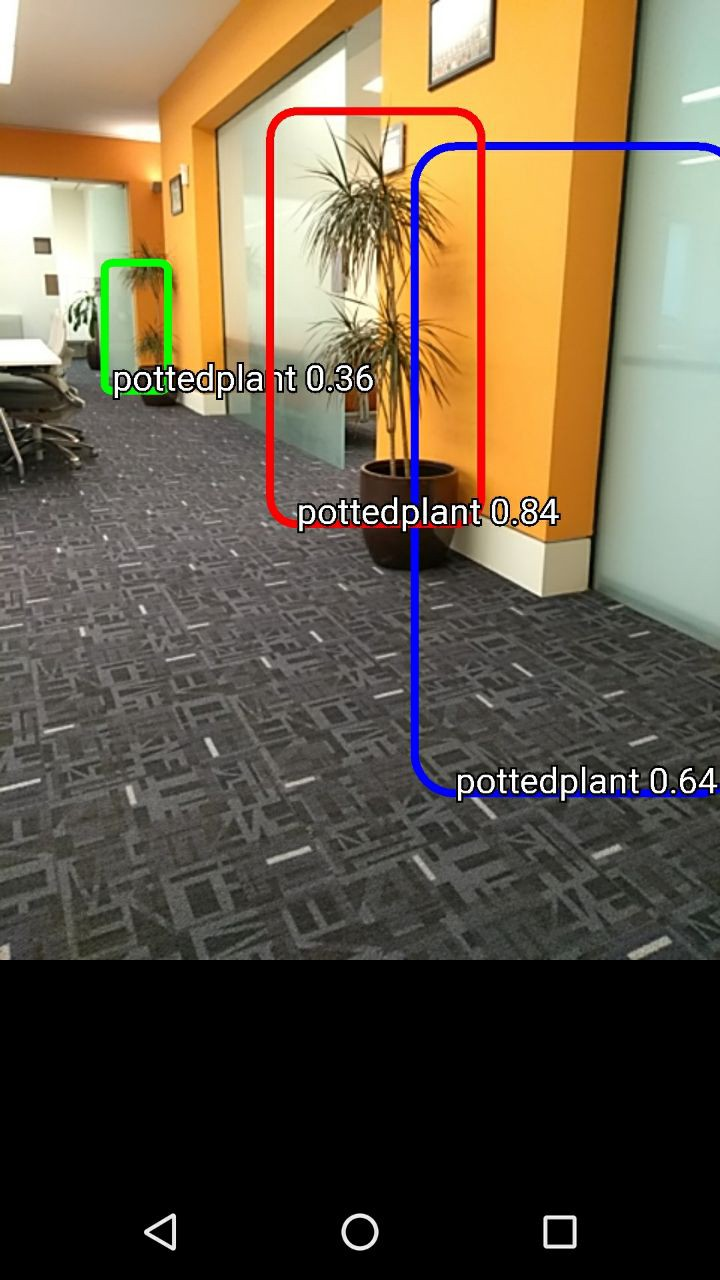
\includegraphics[width=.5\linewidth]{figures/test_6.jpeg}
%  \caption{DeepFlow IOU}
%  \label{fig:DeepFlow_IOU}
%\end{subfigure}
%\caption{DeepFlow Test}
%\label{fig:deep_accuracy}
%\end{figure}

\section{Object Detection Test}

To evaluate how effective is our algorithm in terms of its detection ability, a standard test was set up. We place different objects at specific distances from the drone’s onboard camera to calculate and record the number of seconds in which an object has been detected when there has been movement. We also calculate the number of seconds that the object has not been detected because movement has not been detected, and the seconds in which the algorithm has detected an object as false positive.  For the calculation of the seconds a cell phone stop watch has been used and it has been calculated approximately the seconds in which the algorithm does not detect the object or gives a false positive with human supervision, these data will therefore be totally approximated taking into account the error caused by human visual perception (0.2s). These last times have also been calculated with timer and has taken into account the treatment of experimental errors using the following formulas:

\begin{itemize}
	\item $ Arithmetic  Mean  = \overline{x} =  {\frac{\sum_{i=1}^{n} x_i }{n}} $ 
	\item $ Standard  Deviation  =  \sigma =  {\sqrt{\frac{n}{n -1}*{(\bar{x} - {x_i})^2}}} $ 
	\item $ Accidental  Error  = \varepsilon{_{acc}} =  {\frac{\sigma}{\sqrt{n}}} $ 	
	\item $ Instrument  Error  = \varepsilon{_{ins}} =  {0.01s} $ 	
	\item $ Human  Error  = \varepsilon{_{hum}} =  {0.02s} $ 	
	\item $ Total  Error  = \varepsilon{_{tot}}=  {\sqrt{e_{acc}^{2} + e_{ins}^{2}}} $ 		 
\end{itemize}

\section{Test 1}
The first test for detecting objects was made at a distance of 1m. The result is shown in the image itself by trimming the region representing the zone that is detected. The results obtained are shown in the following table in figure \ref{object_table_1}:

\begin{figure}[ht]
\centering
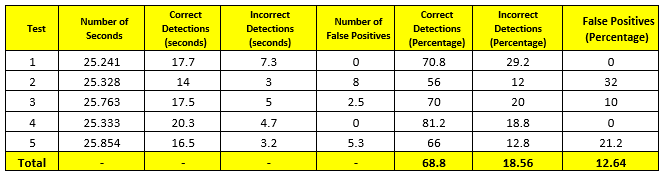
\includegraphics[scale=0.8]{figures/test_table_1.png}
\caption{Object Detection test 1}
\label{object_table_1}
\end{figure}

\pagebreak
\begin{itemize}
	\item $ \overline{x} = \frac{25.241 +  25.328 + 25.763  + 25.333 +  25.854} {5} = \frac{127.519}{5} = 25.504s $ 	
	\item $ \sigma =  {\sqrt{\frac{(25.241 - 25.504)^2 +  (25.328 - 25.504)^2 + (25.763 - 25.504)^2  + (25.333 - 25.504)^2+  (25.854 - 25.504)^2}{5 - 1}}} = 0.282s$
	\item $\varepsilon{_{acc}} =  {\frac{0.282}{\sqrt{5}}} = 0.126s$
	\item $\varepsilon{_{tot}}=  {\sqrt{0.126^{2} + 0.01^{2}}} = 0.126s$
	\item $ \varepsilon{_{ins}} =  {0.01s} $ 	
\end{itemize}

In this test, we have taken samples every \begin{math}25.000\pm0.126s\end{math}. With the algorithm of detecting objects by movement in 1m we see that it is able to detect the object that is being moved in question with a success of 68.8\%. The calculation of time with motion detection is very approximate since it is complicated to process the pixel differences continuously and sometimes false positives \begin{math}(0.3\pm0.2 s)\end{math} and \begin{math}(0.4\pm0.2 s)\end{math} by the movement itself the drone.


\section{Test 2}
The second test of detecting objects was carried out at a distance of 3m. with the same conditions that were already mentioned previously. The results obtained are shown in the table of figure \ref{object_table_2} below:

\begin{figure}[ht]
\centering
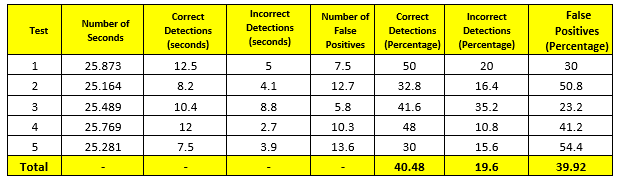
\includegraphics[scale=0.8]{figures/test_table_2.png}
\caption{Object Detection test 2}
\label{object_table_2}
\end{figure}

\pagebreak
\begin{itemize}
	\item $ \overline{x} = \frac{25.873 +  25.164 + 25.489  + 25.769 +  25.281} {5} = \frac{127.576}{5} = 25.515s $ 	
	\item $ \sigma =  {\sqrt{\frac{(25.873 - 25.515)^2 +  (25.164 - 25.515)^2 + (25.489 - 25.515)^2  + (25.769 - 25.515)^2+  (25.281 - 25.515)^2}{5 - 1}}} = 0.305s$
 	\item $\varepsilon{_{acc}} =  {\frac{0.305}{\sqrt{5}}} = 0.136s$
	\item $\varepsilon{_{tot}}=  {\sqrt{ 0.305s^{2} + 0.01^{2}}} = 0.136s$
	\item $ \varepsilon{_{ins}} =  {0.01s} $ 	
\end{itemize}

In this test, we have taken samples every \begin{math}25.000\pm0.136s\end{math}. The results are very similar to those of the previous test. In this case the probability of success is 40.48\% and the false positives were produced with approximate times of \begin{math} 0.3\pm0.2s\end{math}.


\section{Test 3}
The third test was carried out at a distance of 4m. under the same conditions that were mentioned previously. The results obtained are shown in the figure \ref{object_table_3} of the table below:

\begin{figure}[h]
\centering
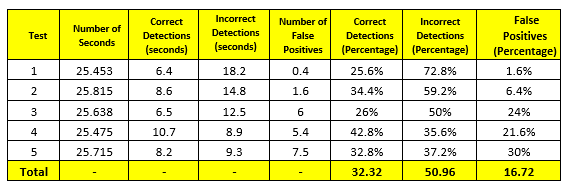
\includegraphics[scale=0.8]{figures/test_table_3.png}
\caption{Object Detection test 3}
\label{object_table_3}
\end{figure}

\pagebreak
\begin{itemize}
	\item $ \overline{x} = \frac{25.453 +  25.815 + 25.638  + 25.475 + 25.715} {5} = \frac{126.595}{5} = 25.319s $ 	
	\item $ \sigma =  {\sqrt{\frac{(25.453 - 25.319)^2 +  (25.815 - 25.319)^2 + (25.638 - 25.319)^2  + (25.475 - 25.319)^2+  ( 25.715 - 25.319)^2}{5 - 1}}} = 0.449s$
	\item $\varepsilon{_{acc}} =  {\frac{0.449}{\sqrt{5}}} = 0.201s$
	\item $ \varepsilon{_{ins}} =  {0.01s} $ 
\end{itemize}

In this test, we have taken samples every \begin{math}25.000\pm0.225 s.\end{math} With a distance of 4m. the detection test gets worse results than the previous ones. This is because the drone having a greater distance, the connection loses intensity and sometimes more temporal lapses occur. In addition, by having more field of view, the algorithm detects the most pixelated object so it is more difficult to find the characteristics of the object. Several temporal lapses of approximately \begin{math}0.3\pm0.2 s\end{math}, \begin{math}0.2\pm0.2 s\end{math} and \begin{math}0.8\pm0.2 s\end{math} occur. In this case, we obtain a 32.32\% success that is still an acceptable percentage and therefore continues to provide reliability to the algorithm.


\section{Recognition test}

\section{Test 1}
The first test for object recognition was made by placing a bottle in front of the camera and gradually move it. The image has been classified with three different distances of 1m, 3m and 4m. The result is displayed in a ranking of 5 probabilities where the object being viewed is classified. The results obtained are reflected in the table in figure \ref{classification_table} below: 


\begin{figure}[ht]
\centering
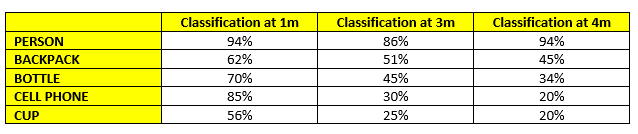
\includegraphics[scale=0.8]{figures/recognition_table_1.png}
\caption{Classification results at difference distances}
\label{classification_table}
\end{figure}

Since the object recognition did not depend strictly on the algorithms, the results were obtained in order to know the optimal distance to obtain data coherent with the classification of the API of the neural network. If we analyze the total results obtained, we see that it has the capacity to obtain valid results for objects that are at a distance of 1 to 6 meters, although with really low probability (uncertainty). For objects that are at a distance of 7 meters or more, the results are very low, but always providing a response. In addition, it should be noted that the recognition API returned very exact results in terms of the type of object. In terms of moving images, the results are not so good at times because the captures are produced with a very fine blurry layer (due to movement) which provides some inaccurate results.


\section{Tracking Test}

The objective in this test is to get the drone to move with the object that is being detected so that the maneuvers follow the following flight pattern:

\begin{enumerate}
\item Raise the flight
\item Detect object.
\item Stay stable for a few seconds.
\item Move the object so that the drone follows an upward movement.
\item Move the object so that the drone follows a downward movement.
\item Move the object so that the drone follows a movement to the right.
\item Move the object so that the drone follows a leftward movement.
\item Follow a circular motion surrounding the drone so that it can perform a 360-degree turn.
\item Land.
\end{enumerate}

We must be aware to see when the drone performs any of the actions correctly in a timed period of time and will be marked as done or not. The time will stop the moment the drone completes the route, stops responding to the commands or loses the connection.

\section{Test 1}
The first test of tracking was done moving a bottle in front of the drone’s onboard camera with the parameters that are reflected in Table 3.40. The values of Amin and Amax have been defined from the most optimal distance (1.5 - 3m) that allows the drone to detect the object more easily and allow it to center the object in the middle of the camera.

\begin{figure}[ht]
\centering
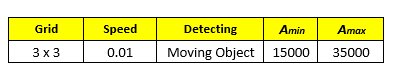
\includegraphics[scale=0.8]{figures/tracking_test_settings_1.png}
\caption{tracking test setup}
\label{tracking_test_setup}
\end{figure}

The results obtained are shown in firgure \ref{} in Table below. To better understand the behavior, a box has been defined per table in which the number of the action to be performed is displayed and whether it has been executed correctly or not.

\begin{figure}[ht]
\centering
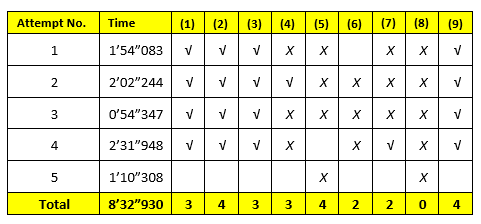
\includegraphics[scale=0.8]{figures/tracking_test_results_1.png}
\caption{tracking test results}
\label{tracking_test_results_1}
\end{figure}

from the table above, we can see that:

\begin{itemize}
\item Attempt No. 1: Does not correctly detect the object being moved. Detects several false positives.
\item Attempt No. 2: It begins to detect the moving object, but the kinetic itself makes it lose stability.
\item Attempt No. 3: Same as the second attempt.
\item Attempt No. 4: Same as the first attempt.
\item Attempt No. 5: Same as the first attempt.
\end{itemize}

\section{Test 2}

The second test of tracking was carried out with the parameters that are reflected in Table in figure \ref{tracking_test_setup}:

\begin{figure}[ht]
\centering
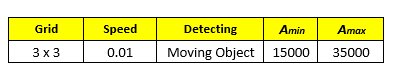
\includegraphics[scale=0.8]{figures/tracking_test_settings_1.png}
\caption{tracking test setup}
\label{tracking_test_setup}
\end{figure}

Results are shown in the the figure \ref{tracking_test_results_2} of the table below:

\begin{figure}[ht]
\centering
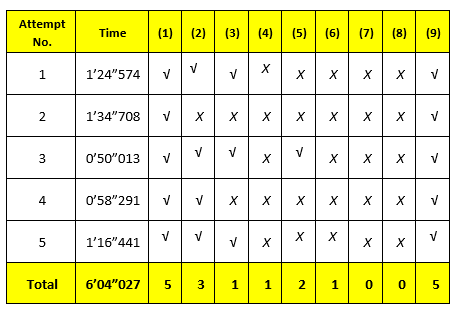
\includegraphics[scale=0.8]{figures/tracking_test_results_2.png}
\caption{tracking test results}
\label{tracking_test_results_2}
\end{figure}

Results are very similar to the first attempt for which as a future work commands sent to drone have to be improved as we detect and track objects:

\begin{itemize}
\item Attempt No. 1: When it detects the object, it doesn’t move. Even though, the algorithm is actually tracking.
\item Attempt No. 2: It does not detect the object and many false positives occur.
\item Attempt No. 3: Similar to the first attempt. False positives cause the object to not move properly.
\item Attempt No. 4: Does not correctly detect the object. It loses connection and therefore stability.
\item Attempt No. 5: We can detect Object Motions clearly but drone doesn’t move.
\end{itemize}

In general, when tracking detection problems persist. Most false positives occur because the camera picks up its own motions and confuses the plane. In the tracking method, we see that the results are not optimal and that it is not possible to perform almost any actions, due to the false positives of the cinematic movement of the drone and its own stabilizer. In addition, the tests were shorter because it suffered continually due to the heaviness and the delay of the algorithm itself.


%%%%%%%%%%%%%%%%%%%%%%%%%%%%%%%%%%%%%%%%%%%%%%%%%%%
%
%  New template code for TAMU Theses and Dissertations starting Fall 2012.  
%  For more info about this template or the 
%  TAMU LaTeX User's Group, see http://www.howdy.me/.
%
%  Author: Wendy Lynn Turner 
%	 Version 1.0 
%  Last updated 8/5/2012
%
%%%%%%%%%%%%%%%%%%%%%%%%%%%%%%%%%%%%%%%%%%%%%%%%%%%
%%%%%%%%%%%%%%%%%%%%%%%%%%%%%%%%%%%%%%%%%%%%%%%%%%%%%%%%%%%%%%%%%%%%%%
%%                           SECTION IV
%%%%%%%%%%%%%%%%%%%%%%%%%%%%%%%%%%%%%%%%%%%%%%%%%%%%%%%%%%%%%%%%%%%%%

\chapter{\uppercase{Seismic Data Analytics Platform}}

In oil and gas companies, the data analytics software is not only used by scientists and researchers, but also the employees who do not have the background of computer science. To allow those users to browse the seismic data and to generate analytics result, the researchers developed some user-friendly utilities on top of Seismic Data Analytics SDK to simplify the way for deploying general purpose applications on Spark-Hadoop platform, which include a distributed data server for remote data access, the web interfaces for remote data visualization and user-defined workflow. With these tools, the users, not only the developers, are able to easily facilitate their works with this Seismic Data Analytics Platform in minimal efforts.


\section{Data Server and Remote Web Visualization}

In petroleum industry, an important application scenario is data visualization, which allows user to browse and analyze seismology features of seismic data in 3D spacing. With visualization tools, computer renders the seismic data to 3D graphic views and allows user to browse and manipulate the graph along any direction, which inspired the geophysicists and data scientists to develop various of useful models. However,traditional visualization tools in industry are only capable of handling small datasets, or render only few segments of the big datasets at a time. The performance of  big dataset visualization has long been the critical bottleneck of regular workflow of industry.

To resolve this problem, the researchers developed a web-based remote data visualization service which was able to load and render the seismic data for 3D visualization in real-time. Figure \ref{visualization_framework} shows the framework of this service. 

\begin{figure}[h]
\centering
\includegraphics[scale=0.3]{figures/visualization_framework.png}
\caption{The Framework of Remote Web Visualization Service}
\label{visualization_framework}
\end{figure}

This solution was developed on top of Seismic Data Analytics SDK APIs and FEI Digital Rock Visualization Packages. The researchers designed and implemented the DataServer service on top of Seismic Data Analytics SDK, which could load big seismic datasets from HDFS, transpose and store them to SeismicRDD in backends then feed the requested data in any direction to FEI visualization service in real-time. The FEI Digital Rock Visualization package was developed by FEI, the company which has been focus on featuring Digital Rock technology and solutions many years \cite{FEICompany}. 

Finally, the output rendered data view is presented through web interface and allows user to browse and manipulate in any direction. With this solution, users do not need to install complicated visualization tools and packages since the platform handles everything on server-side. More importantly, the performance of rendering big seismic data is improved and scalable after facilitated by Seismic Data Analytics SDK. Figure \ref{visualization} shows the web interface of this solution.

\begin{figure}[h]
\centering
\includegraphics[scale=0.3]{figures/visualization.png}
\caption{Visualization Web Interface}
\label{visualization}
\end{figure}


\section{Web-based Workflow Platform}

Another service developed was a web-based workflow platform, which provides a user-friendly web interface to make cloud platform easy to use without programming, with which users could create workflow with drag and drop, could run the pre-built workflow and browse the results via the visualization service. This workflow web service was developed on top of the open-source project Clowdflows \cite{Clowdflows}, which provides a Django based web application framework to develop and manage customized widgets and workflows conveniently. As a free and open source web framework developed in Python, Django follows the classic Model, View and Controller (MVC) architectural pattern, so this application is suitable for interacting with both cloud service and web client.

The client side view of workflow is shown as Figure \ref{workflow}. Users could select widgets and specify seismic data files as input to construct their workflows. Each widget in the workflow view is an independent application component which could be implemented on top of Seismic Data Analytics SDK. A widget acquires at least one port as input or output thus multiple widgets are able to be combined to a workflow by multiple pipelines which connect the ports of all widgets. Each pipeline in the workflow view indicates a data communication, which transports data between widgets and drives the execution of whole workflow. The workflow framework implemented by Python code includes Django views (GUI), Django models (widgets data management) and topological sorting algorithm (connections check).  The data files are stored in HDFS of the cloud platform and could be browsed and selected from the navigation trees on the editor page.

\begin{figure}[h]
\centering
\includegraphics[scale=0.3]{figures/workflow.png}
\caption{Workflow Web Interface}
\label{workflow}
\end{figure}


%%%%%%%%%%%%%%%%%%%%%%%%%%%%%%%%%%%%%%%%%%%%%%%%%%%
%
%  New template code for TAMU Theses and Dissertations starting Fall 2012.  
%  For more info about this template or the 
%  TAMU LaTeX User's Group, see http://www.howdy.me/.
%
%  Author: Wendy Lynn Turner 
%	 Version 1.0 
%  Last updated 8/5/2012
%
%%%%%%%%%%%%%%%%%%%%%%%%%%%%%%%%%%%%%%%%%%%%%%%%%%%
%%%%%%%%%%%%%%%%%%%%%%%%%%%%%%%%%%%%%%%%%%%%%%%%%%%%%%%%%%%%%%%%%%%%%%
%%                           SECTION VI
%%%%%%%%%%%%%%%%%%%%%%%%%%%%%%%%%%%%%%%%%%%%%%%%%%%%%%%%%%%%%%%%%%%%%



\chapter{\uppercase{Conclusions and Future Work}}

The thesis presents the implementation and adaptation of an object detection and tracking system using 3DRobotics Solo Drone. For each algorithm, we have tried to analyze the ability and the functioning of how they act in a drone, ie, these algorithms were evaluated to determine if the use of a drone was conceptually feasible to perform any of these functions and thus to choose how to form the system of autonomous behavior more suitable for it.

During the course of the project, there have been several drawbacks and limitations. Initially, we use a DJI Matrice 100 drone which does not seem to be the most suitable vehicle for this type of behavior within closed spaces, because of both, its physiognomy and the materials  which it is made with. However, when it comes to flying, it is quite sensitive to external factors. The sensor itself that stabilizes the drone, is very affected although it is not receiving any command of movement. We switched to 3DRobotics Solo Drone which seemed to be better but at the time of implementing and testing the algorithms, there were many problems, such as difficulties accessing the onboard camera from the central PC connected to the drone, because there were exceptions of sockets where it didn't find the /video0/ function. These problems caused the drone to reboot everytime you tried to run a script to access the main camera.

Object recognition and Tracking is not a trivial task when incorporating the necessary mechanisms that artificial intelligence needs. Even if we use the best libraries that incorporate the faster and more efficient methods would be possible to achieve. And is that each program has its own requirements, the most important is to have a good focus on the operation of algorithms based on tests, rather than a strictly theoretical basis.

Looking back in time, there are certain things that could have been approached differently in order to get better results at the end of the project, such as a more comprehensive planning phase. Given that my experience in the field of computer vision was very light, it has taken me a great deal of effort and time to learn and read about OpenCV, OpenTLD, TLD, TensorFlow,  and everything that the theory of computer vision entails. In addition to learning, incorporating, and adapting mechanisms of robotics in a drone, which requires to fully understand how their sensors and associated invariant properties work. However, we will continue to work hard to improve our algorithm results in the mobile platforms increase the number of frames and how fast it can detect and track an object as well as improving frame rate in a workstation working only with a CPU.

%%%%%%%%%%%%%%%%%%%%%%%%%%%%%%%%%%%%%%%%%%%%%%%%%%%%%%%
%\begin{figure}[H]
%\centering
%\includegraphics[scale=.50]{figures/Penguins.jpg}
%\caption{Another TAMU figure}
%\label{fig:tamu-fig4}
%\end{figure}
%%%%%%%%%%%%%%%%%%%%%%%%%%%%%%%%%%%%%%%%%%%%%%%%%%%%%%%




%fix spacing in bibliography, if any...
%%%%%%%%%%%%%%%%%%%%%%%%%%%%%%%%%%%%%%%%%%%%%%%%%%%%%%%%%%%%%
\let\oldbibitem\bibitem
\renewcommand{\bibitem}{\setlength{\itemsep}{0pt}\oldbibitem}
%%%%%%%%%%%%%%%%%%%%%%%%%%%%%%%%%%%%%%%%%%%%%%%%%%%%%%%%%%%%%%%
%%%%%%%%%%%%%%%%%%%%%%%%%%%%%%%%%%%%%%%%%%%%%%%%%%%
%
%  New template code for TAMU Theses and Dissertations starting Fall 2012.  
%  For more info about this template or the 
%  TAMU LaTeX User's Group, see http://www.howdy.me/.
%
%  Author: Wendy Lynn Turner 
%	 Version 1.0 
%  Last updated 8/5/2012
%
%%%%%%%%%%%%%%%%%%%%%%%%%%%%%%%%%%%%%%%%%%%%%%%%%%%


%%%%%%%%%%%%%%%%%%%%%%%%%%%%%%%%%%%%%%%%%%%%%%%%%%%%%%%%%%%%%%%%%%%%%%
%%                           REFERENCES 
%%%%%%%%%%%%%%%%%%%%%%%%%%%%%%%%%%%%%%%%%%%%%%%%%%%%%%%%%%%%%%%%%%%%%

\phantomsection
\addcontentsline{toc}{chapter}{REFERENCES}

\renewcommand{\bibname}{{REFERENCES}}

\bibliographystyle{ieeetr}
\bibliography{references}

%%%%%%%%%%%%%%%%%%%%%%%%%%%%%%%%%%%%%%%%%%%%%%%%%%%
%
%  New template code for TAMU Theses and Dissertations starting Fall 2012.  
%  For more info about this template or the 
%  TAMU LaTeX User's Group, see http://www.howdy.me/.
%
%  Author: Wendy Lynn Turner 
%	 Version 1.0 
%  Last updated 8/5/2012
%
%%%%%%%%%%%%%%%%%%%%%%%%%%%%%%%%%%%%%%%%%%%%%%%%%%%
%%%%%%%%%%%%%%%%%%%%%%%%%%%%%%%%%%%%%%%%%%%%%%%%%%%%%%%%%%%%%%%%%%%%%%
%%                           SECTION IV
%%%%%%%%%%%%%%%%%%%%%%%%%%%%%%%%%%%%%%%%%%%%%%%%%%%%%%%%%%%%%%%%%%%%%

\chapter{\uppercase{Seismic Data Analytics Platform}}

In oil and gas companies, the data analytics software is not only used by scientists and researchers, but also the employees who do not have the background of computer science. To allow those users to browse the seismic data and to generate analytics result, the researchers developed some user-friendly utilities on top of Seismic Data Analytics SDK to simplify the way for deploying general purpose applications on Spark-Hadoop platform, which include a distributed data server for remote data access, the web interfaces for remote data visualization and user-defined workflow. With these tools, the users, not only the developers, are able to easily facilitate their works with this Seismic Data Analytics Platform in minimal efforts.


\section{Data Server and Remote Web Visualization}

In petroleum industry, an important application scenario is data visualization, which allows user to browse and analyze seismology features of seismic data in 3D spacing. With visualization tools, computer renders the seismic data to 3D graphic views and allows user to browse and manipulate the graph along any direction, which inspired the geophysicists and data scientists to develop various of useful models. However,traditional visualization tools in industry are only capable of handling small datasets, or render only few segments of the big datasets at a time. The performance of  big dataset visualization has long been the critical bottleneck of regular workflow of industry.

To resolve this problem, the researchers developed a web-based remote data visualization service which was able to load and render the seismic data for 3D visualization in real-time. Figure \ref{visualization_framework} shows the framework of this service. 

\begin{figure}[h]
\centering
\includegraphics[scale=0.3]{figures/visualization_framework.png}
\caption{The Framework of Remote Web Visualization Service}
\label{visualization_framework}
\end{figure}

This solution was developed on top of Seismic Data Analytics SDK APIs and FEI Digital Rock Visualization Packages. The researchers designed and implemented the DataServer service on top of Seismic Data Analytics SDK, which could load big seismic datasets from HDFS, transpose and store them to SeismicRDD in backends then feed the requested data in any direction to FEI visualization service in real-time. The FEI Digital Rock Visualization package was developed by FEI, the company which has been focus on featuring Digital Rock technology and solutions many years \cite{FEICompany}. 

Finally, the output rendered data view is presented through web interface and allows user to browse and manipulate in any direction. With this solution, users do not need to install complicated visualization tools and packages since the platform handles everything on server-side. More importantly, the performance of rendering big seismic data is improved and scalable after facilitated by Seismic Data Analytics SDK. Figure \ref{visualization} shows the web interface of this solution.

\begin{figure}[h]
\centering
\includegraphics[scale=0.3]{figures/visualization.png}
\caption{Visualization Web Interface}
\label{visualization}
\end{figure}


\section{Web-based Workflow Platform}

Another service developed was a web-based workflow platform, which provides a user-friendly web interface to make cloud platform easy to use without programming, with which users could create workflow with drag and drop, could run the pre-built workflow and browse the results via the visualization service. This workflow web service was developed on top of the open-source project Clowdflows \cite{Clowdflows}, which provides a Django based web application framework to develop and manage customized widgets and workflows conveniently. As a free and open source web framework developed in Python, Django follows the classic Model, View and Controller (MVC) architectural pattern, so this application is suitable for interacting with both cloud service and web client.

The client side view of workflow is shown as Figure \ref{workflow}. Users could select widgets and specify seismic data files as input to construct their workflows. Each widget in the workflow view is an independent application component which could be implemented on top of Seismic Data Analytics SDK. A widget acquires at least one port as input or output thus multiple widgets are able to be combined to a workflow by multiple pipelines which connect the ports of all widgets. Each pipeline in the workflow view indicates a data communication, which transports data between widgets and drives the execution of whole workflow. The workflow framework implemented by Python code includes Django views (GUI), Django models (widgets data management) and topological sorting algorithm (connections check).  The data files are stored in HDFS of the cloud platform and could be browsed and selected from the navigation trees on the editor page.

\begin{figure}[h]
\centering
\includegraphics[scale=0.3]{figures/workflow.png}
\caption{Workflow Web Interface}
\label{workflow}
\end{figure}


%%%%%%%%%%%%%%%%%%%%%%%%%%%%%%%%%%%%%%%%%%%%%%%%%%%
%
%  New template code for TAMU Theses and Dissertations starting Fall 2012.  
%  For more info about this template or the 
%  TAMU LaTeX User's Group, see http://www.howdy.me/.
%
%  Author: Wendy Lynn Turner 
%	 Version 1.0 
%  Last updated 8/5/2012
%
%%%%%%%%%%%%%%%%%%%%%%%%%%%%%%%%%%%%%%%%%%%%%%%%%%%

\begin{appendices}
\titleformat{\chapter}{\centering\normalsize}{APPENDIX \thechapter}{0em}{\vskip .5\baselineskip\centering}
\renewcommand{\appendixname}{APPENDIX}

%%%%%%%%%%%%%%%%%%%%%%%%%%%%%%%%%%%%%%%%%%%%%%%%%%%
%
%  New template code for TAMU Theses and Dissertations starting Fall 2012.  
%  For more info about this template or the 
%  TAMU LaTeX User's Group, see http://www.howdy.me/.
%
%  Author: Wendy Lynn Turner 
%	 Version 1.0 
%  Last updated 8/5/2012
%
%%%%%%%%%%%%%%%%%%%%%%%%%%%%%%%%%%%%%%%%%%%%%%%%%%%

%%%%%%%%%%%%%%%%%%%%%%%%%%%%%%%%%%%%%%%%%%%%%%%%%%%%%%%%%%%%%%%%%%%%%%
%%                           APPENDIX A 
%%%%%%%%%%%%%%%%%%%%%%%%%%%%%%%%%%%%%%%%%%%%%%%%%%%%%%%%%%%%%%%%%%%%%

\phantomsection

\chapter{\uppercase{Code Implementation}}

\begin{lstlisting}
//inference.py
import inspect
import tensorflow as tf
import tensorflow.contrib.slim as slim
from ..yolo.function import leaky_relu
from .function import reorg


def tiny(net, classes, num_anchors, training=False, center=True):
    def batch_norm(net):
        net = slim.batch_norm(net, center=center, scale=True, epsilon=1e-5, is_training=training)
        if not center:
            net = tf.nn.bias_add(net, slim.variable('biases', shape=[tf.shape(net)[-1]], initializer=tf.zeros_initializer()))
        return net
    scope = __name__.split('.')[-2] + '_' + inspect.stack()[0][3]
    net = tf.identity(net, name='%s/input' % scope)
    with slim.arg_scope([slim.layers.conv2d], kernel_size=[3, 3], weights_initializer=tf.truncated_normal_initializer(stddev=0.1), normalizer_fn=batch_norm, activation_fn=leaky_relu), slim.arg_scope([slim.layers.max_pool2d], kernel_size=[2, 2], padding='SAME'):
        index = 0
        channels = 16
        for _ in range(5):
            net = slim.layers.conv2d(net, channels, scope='%s/conv%d' % (scope, index))
            net = slim.layers.max_pool2d(net, scope='%s/max_pool%d' % (scope, index))
            index += 1
            channels *= 2
        net = slim.layers.conv2d(net, channels, scope='%s/conv%d' % (scope, index))
        net = slim.layers.max_pool2d(net, stride=1, scope='%s/max_pool%d' % (scope, index))
        index += 1
        channels *= 2
        net = slim.layers.conv2d(net, channels, scope='%s/conv%d' % (scope, index))
        index += 1
        net = slim.layers.conv2d(net, channels, scope='%s/conv%d' % (scope, index))
    net = slim.layers.conv2d(net, num_anchors * (5 + classes), kernel_size=[1, 1], activation_fn=None, scope='%s/conv' % scope)
    net = tf.identity(net, name='%s/output' % scope)
    return scope, net

TINY_DOWNSAMPLING = (2 ** 5, 2 ** 5)


def _tiny(net, classes, num_anchors, training=False):
    return tiny(net, classes, num_anchors, training, False)

_TINY_DOWNSAMPLING = (2 ** 5, 2 ** 5)


def darknet(net, classes, num_anchors, training=False, center=True):
    def batch_norm(net):
        net = slim.batch_norm(net, center=center, scale=True, epsilon=1e-5, is_training=training)
        if not center:
            net = tf.nn.bias_add(net, slim.variable('biases', shape=[tf.shape(net)[-1]], initializer=tf.zeros_initializer()))
        return net
    scope = __name__.split('.')[-2] + '_' + inspect.stack()[0][3]
    net = tf.identity(net, name='%s/input' % scope)
    with slim.arg_scope([slim.layers.conv2d], kernel_size=[3, 3], normalizer_fn=batch_norm, activation_fn=leaky_relu), slim.arg_scope([slim.layers.max_pool2d], kernel_size=[2, 2], padding='SAME'):
        index = 0
        channels = 32
        for _ in range(2):
            net = slim.layers.conv2d(net, channels, scope='%s/conv%d' % (scope, index))
            net = slim.layers.max_pool2d(net, scope='%s/max_pool%d' % (scope, index))
            index += 1
            channels *= 2
        for _ in range(2):
            net = slim.layers.conv2d(net, channels, scope='%s/conv%d' % (scope, index))
            index += 1
            net = slim.layers.conv2d(net, channels / 2, kernel_size=[1, 1], scope='%s/conv%d' % (scope, index))
            index += 1
            net = slim.layers.conv2d(net, channels, scope='%s/conv%d' % (scope, index))
            net = slim.layers.max_pool2d(net, scope='%s/max_pool%d' % (scope, index))
            index += 1
            channels *= 2
        net = slim.layers.conv2d(net, channels, scope='%s/conv%d' % (scope, index))
        index += 1
        net = slim.layers.conv2d(net, channels / 2, kernel_size=[1, 1], scope='%s/conv%d' % (scope, index))
        index += 1
        net = slim.layers.conv2d(net, channels, scope='%s/conv%d' % (scope, index))
        index += 1
        net = slim.layers.conv2d(net, channels / 2, kernel_size=[1, 1], scope='%s/conv%d' % (scope, index))
        index += 1
        net = slim.layers.conv2d(net, channels, scope='%s/conv%d' % (scope, index))
        passthrough = tf.identity(net, name=scope + '/passthrough')
        net = slim.layers.max_pool2d(net, scope='%s/max_pool%d' % (scope, index))
        index += 1
        channels *= 2
        # downsampling finished
        net = slim.layers.conv2d(net, channels, scope='%s/conv%d' % (scope, index))
        index += 1
        net = slim.layers.conv2d(net, channels / 2, kernel_size=[1, 1], scope='%s/conv%d' % (scope, index))
        index += 1
        net = slim.layers.conv2d(net, channels, scope='%s/conv%d' % (scope, index))
        index += 1
        net = slim.layers.conv2d(net, channels / 2, kernel_size=[1, 1], scope='%s/conv%d' % (scope, index))
        index += 1
        net = slim.layers.conv2d(net, channels, scope='%s/conv%d' % (scope, index))
        index += 1
        net = slim.layers.conv2d(net, channels, scope='%s/conv%d' % (scope, index))
        index += 1
        net = slim.layers.conv2d(net, channels, scope='%s/conv%d' % (scope, index))
        index += 1
        with tf.name_scope(scope):
            _net = reorg(passthrough)
        net = tf.concat([_net, net], 3, name='%s/concat%d' % (scope, index))
        net = slim.layers.conv2d(net, channels, scope='%s/conv%d' % (scope, index))
    net = slim.layers.conv2d(net, num_anchors * (5 + classes), kernel_size=[1, 1], activation_fn=None, scope='%s/conv' % scope)
    net = tf.identity(net, name='%s/output' % scope)
    return scope, net

DARKNET_DOWNSAMPLING = (2 ** 5, 2 ** 5)


def _darknet(net, classes, num_anchors, training=False):
    return darknet(net, classes, num_anchors, training, False)

_DARKNET_DOWNSAMPLING = (2 ** 5, 2 ** 5)

\end{lstlisting}

\pagebreak
\begin{lstlisting}
//functions.py
import numpy as np
import tensorflow as tf


def reorg(net, stride=2, name='reorg'):
    batch_size, height, width, channels = net.get_shape().as_list()
    _height, _width, _channel = height // stride, width // stride, channels * stride * stride
    with tf.name_scope(name) as name:
        net = tf.reshape(net, [batch_size, _height, stride, _width, stride, channels])
        net = tf.transpose(net, [0, 1, 3, 2, 4, 5]) # batch_size, _height, _width, stride, stride, channels
        net = tf.reshape(net, [batch_size, _height, _width, -1], name=name)
    return net


def main():
    image = [
        (0, 1, 0, 1),
        (2, 3, 2, 3),
        (0, 1, 0, 1),
        (2, 3, 2, 3),
    ]
    image = np.expand_dims(image, 0)
    image = np.expand_dims(image, -1)
    with tf.Session() as sess:
        ph_image = tf.placeholder(tf.uint8, image.shape)
        images = sess.run(reorg(ph_image), feed_dict={ph_image: image})
    for i, image in enumerate(np.transpose(images[0], [2, 0, 1])):
        data = np.unique(image)
        assert len(data) == 1
        assert data[0] == i

if __name__ == '__main__':
    main()
\end{lstlisting}

\pagebreak
\begin{lstlisting}
//preprocess.py
import inspect
import numpy as np
import tensorflow as tf


def per_image_standardization(image):
    stddev = np.std(image)
    return (image - np.mean(image)) / max(stddev, 1.0 / np.sqrt(np.multiply.reduce(image.shape)))


def random_crop(image, objects_coord, width_height, scale=1):
    assert 0 < scale <= 1
    section = inspect.stack()[0][3]
    with tf.name_scope(section):
        xy_min = tf.reduce_min(objects_coord[:, :2], 0)
        xy_max = tf.reduce_max(objects_coord[:, 2:], 0)
        margin = width_height - xy_max
        shrink = tf.random_uniform([4], maxval=scale) * tf.concat([xy_min, margin], 0)
        _xy_min = shrink[:2]
        _wh = width_height - shrink[2:] - _xy_min
        objects_coord = objects_coord - tf.tile(_xy_min, [2])
        _xy_min_ = tf.cast(_xy_min, tf.int32)
        _wh_ = tf.cast(_wh, tf.int32)
        image = tf.image.crop_to_bounding_box(image, _xy_min_[1], _xy_min_[0], _wh_[1], _wh_[0])
    return image, objects_coord, _wh


def flip_horizontally(image, objects_coord, width):
    section = inspect.stack()[0][3]
    with tf.name_scope(section):
        image = tf.image.flip_left_right(image)
        xmin, ymin, xmax, ymax = objects_coord[:, 0:1], objects_coord[:, 1:2], objects_coord[:, 2:3], objects_coord[:, 3:4]
        objects_coord = tf.concat([width - xmax, ymin, width - xmin, ymax], 1)
    return image, objects_coord


def random_flip_horizontally(image, objects_coord, width, probability=0.5):
    section = inspect.stack()[0][3]
    with tf.name_scope(section):
        pred = tf.random_uniform([]) < probability
        fn1 = lambda: flip_horizontally(image, objects_coord, width)
        fn2 = lambda: (image, objects_coord)
        return tf.cond(pred, fn1, fn2)


def random_grayscale(image, probability=0.5):
    if probability <= 0:
        return image
    section = inspect.stack()[0][3]
    with tf.name_scope(section):
        pred = tf.random_uniform([]) < probability
        fn1 = lambda: tf.tile(tf.image.rgb_to_grayscale(image), [1] * (len(image.get_shape()) - 1) + [3])
        fn2 = lambda: image
        return tf.cond(pred, fn1, fn2)

\end{lstlisting}


\pagebreak
\begin{lstlisting}
//postprocess.py
import numpy as np


def iou(xy_min1, xy_max1, xy_min2, xy_max2):
    assert(not np.isnan(xy_min1).any())
    assert(not np.isnan(xy_max1).any())
    assert(not np.isnan(xy_min2).any())
    assert(not np.isnan(xy_max2).any())
    assert np.all(xy_min1 <= xy_max1)
    assert np.all(xy_min2 <= xy_max2)
    areas1 = np.multiply.reduce(xy_max1 - xy_min1)
    areas2 = np.multiply.reduce(xy_max2 - xy_min2)
    _xy_min = np.maximum(xy_min1, xy_min2) 
    _xy_max = np.minimum(xy_max1, xy_max2)
    _wh = np.maximum(_xy_max - _xy_min, 0)
    _areas = np.multiply.reduce(_wh)
    assert _areas <= areas1
    assert _areas <= areas2
    return _areas / np.maximum(areas1 + areas2 - _areas, 1e-10)


def non_max_suppress(conf, xy_min, xy_max, threshold, threshold_iou):
    _, _, classes = conf.shape
    boxes = [(_conf, _xy_min, _xy_max) for _conf, _xy_min, _xy_max in zip(conf.reshape(-1, classes), xy_min.reshape(-1, 2), xy_max.reshape(-1, 2))]
    for c in range(classes):
        boxes.sort(key=lambda box: box[0][c], reverse=True)
        for i in range(len(boxes) - 1):
            box = boxes[i]
            if box[0][c] <= threshold:
                continue
            for _box in boxes[i + 1:]:
                if iou(box[1], box[2], _box[1], _box[2]) >= threshold_iou:
                    _box[0][c] = 0
    return boxes


\end{lstlisting}


\pagebreak
\begin{lstlisting}
//visualize.py
import itertools
import numpy as np
import matplotlib.pyplot as plt
import matplotlib.patches as patches


def draw_labels(ax, names, width, height, cell_width, cell_height, mask, prob, coords, xy_min, xy_max, areas, rtol=1e-3):
    colors = [prop['color'] for _, prop in zip(names, itertools.cycle(plt.rcParams['axes.prop_cycle']))]
    plots = []
    for i, (_mask, _prob, _coords, _xy_min, _xy_max, _areas) in enumerate(zip(mask, prob, coords, xy_min, xy_max, areas)):
        _mask = _mask.reshape([])
        _coords = _coords.reshape([-1])
        if np.any(_mask) > 0:
            index = np.argmax(_prob)
            iy = i // cell_width
            ix = i % cell_width
            plots.append(ax.add_patch(patches.Rectangle((ix * width / cell_width, iy * height / cell_height), width / cell_width, height / cell_height, linewidth=0, facecolor=colors[index], alpha=.2)))
            #check coords
            offset_x, offset_y, _w_sqrt, _h_sqrt = _coords
            cell_x, cell_y = ix + offset_x, iy + offset_y
            x, y = cell_x * width / cell_width, cell_y * height / cell_height
            _w, _h = _w_sqrt * _w_sqrt, _h_sqrt * _h_sqrt
            w, h = _w * width, _h * height
            x_min, y_min = x - w / 2, y - h / 2
            plots.append(ax.add_patch(patches.Rectangle((x_min, y_min), w, h, linewidth=1, edgecolor=colors[index], facecolor='none')))
            plots.append(ax.annotate(names[index], (x_min, y_min), color=colors[index]))
            #check offset_xy_min and xy_max
            wh = _xy_max - _xy_min
            assert np.all(wh >= 0)
            np.testing.assert_allclose(wh / [cell_width, cell_height], [[_w, _h]], rtol=rtol)
            np.testing.assert_allclose(_xy_min + wh / 2, [[offset_x, offset_y]], rtol=rtol)
    return plots


\end{lstlisting}

\pagebreak
\begin{lstlisting}
//cache.py
import os
import argparse
import configparser
import shutil
import importlib
import pandas as pd
import tensorflow as tf
import utils


def main():
    cachedir = utils.get_cachedir(config)
    os.makedirs(cachedir, exist_ok=True)
    path = os.path.join(cachedir, 'names')
    shutil.copyfile(os.path.expanduser(os.path.expandvars(config.get('cache', 'names'))), path)
    with open(path, 'r') as f:
        names = [line.strip() for line in f]
    name_index = dict([(name, i) for i, name in enumerate(names)])
    datasets = [(os.path.basename(os.path.splitext(path)[0]), pd.read_csv(os.path.expanduser(os.path.expandvars(path)), sep='\t')) for path in config.get('cache', 'datasets').split(':')]
    module = importlib.import_module('utils.data.cache')
    for profile in args.profile:
        path = os.path.join(cachedir, profile + '.tfrecord')
        tf.logging.info('write tfrecords file: ' + path)
        with tf.python_io.TFRecordWriter(path) as writer:
            for name, dataset in datasets:
                tf.logging.info('loading %s %s dataset' % (name, profile))
                func = getattr(module, name)
                for i, row in dataset.iterrows():
                    tf.logging.info('loading data %d (%s)' % (i, ', '.join([k + '=' + str(v) for k, v in row.items()])))
                    func(writer, name_index, profile, row, args.verify)
    tf.logging.info('%s data are saved into %s' % (str(args.profile), cachedir))


def make_args():
    parser = argparse.ArgumentParser()
    parser.add_argument('-c', '--config', nargs='+', default=['config.ini'], help='config file')
    parser.add_argument('-p', '--profile', nargs='+', default=['train', 'val', 'test'])
    parser.add_argument('-v', '--verify', action='store_true')
    parser.add_argument('--level', default='info', help='logging level')
    return parser.parse_args()

if __name__ == '__main__':
    args = make_args()
    config = configparser.ConfigParser()
    utils.load_config(config, args.config)
    if args.level:
        tf.logging.set_verbosity(args.level.upper())
    with tf.Session() as sess:
        main()


\end{lstlisting}

\pagebreak
\begin{lstlisting}
//parse_yolov2.py
import os
import re
import time
import shutil
import argparse
import configparser
import operator
import itertools
import struct
import numpy as np
import pandas as pd
import tensorflow as tf
import model.yolo2.inference as inference
import utils


def transpose_weights(weights, num_anchors):
    ksize1, ksize2, channels_in, _ = weights.shape
    weights = weights.reshape([ksize1, ksize2, channels_in, num_anchors, -1])
    coords = weights[:, :, :, :, 0:4]
    iou = np.expand_dims(weights[:, :, :, :, 4], -1)
    classes = weights[:, :, :, :, 5:]
    return np.concatenate([iou, coords, classes], -1).reshape([ksize1, ksize2, channels_in, -1])


def transpose_biases(biases, num_anchors):
    biases = biases.reshape([num_anchors, -1])
    coords = biases[:, 0:4]
    iou = np.expand_dims(biases[:, 4], -1)
    classes = biases[:, 5:]
    return np.concatenate([iou, coords, classes], -1).reshape([-1])


def transpose(sess, layer, num_anchors):
    v = next(filter(lambda v: v.op.name.endswith('weights'), layer))
    sess.run(v.assign(transpose_weights(sess.run(v), num_anchors)))
    v = next(filter(lambda v: v.op.name.endswith('biases'), layer))
    sess.run(v.assign(transpose_biases(sess.run(v), num_anchors)))


def main():
    model = config.get('config', 'model')
    cachedir = utils.get_cachedir(config)
    with open(os.path.join(cachedir, 'names'), 'r') as f:
        names = [line.strip() for line in f]
    width, height = np.array(utils.get_downsampling(config)) * 13
    anchors = pd.read_csv(os.path.expanduser(os.path.expandvars(config.get(model, 'anchors'))), sep='\t').values
    func = getattr(inference, config.get(model, 'inference'))
    with tf.Session() as sess:
        image = tf.placeholder(tf.float32, [1, height, width, 3], name='image')
        func(image, len(names), len(anchors))
        tf.contrib.framework.get_or_create_global_step()
        tf.global_variables_initializer().run()
        prog = re.compile(r'[_\w\d]+\/conv(\d*)\/(weights|biases|(BatchNorm\/(gamma|beta|moving_mean|moving_variance)))$')
        variables = [(prog.match(v.op.name).group(1), v) for v in tf.global_variables() if prog.match(v.op.name)]
        variables = sorted([[int(k) if k else -1, [v for _, v in g]] for k, g in itertools.groupby(variables, operator.itemgetter(0))], key=operator.itemgetter(0))
        assert variables[0][0] == -1
        variables[0][0] = len(variables) - 1
        variables.insert(len(variables), variables.pop(0))
        with tf.name_scope('assign'):
            with open(os.path.expanduser(os.path.expandvars(args.file)), 'rb') as f:
                major, minor, revision, seen = struct.unpack('4i', f.read(16))
                tf.logging.info('major=%d, minor=%d, revision=%d, seen=%d' % (major, minor, revision, seen))
                for i, layer in variables:
                    tf.logging.info('processing layer %d' % i)
                    total = 0
                    for suffix in ['biases', 'beta', 'gamma', 'moving_mean', 'moving_variance', 'weights']:
                        try:
                            v = next(filter(lambda v: v.op.name.endswith(suffix), layer))
                        except StopIteration:
                            continue
                        shape = v.get_shape().as_list()
                        cnt = np.multiply.reduce(shape)
                        total += cnt
                        tf.logging.info('%s: %s=%d' % (v.op.name, str(shape), cnt))
                        p = struct.unpack('%df' % cnt, f.read(4 * cnt))
                        if suffix == 'weights':
                            ksize1, ksize2, channels_in, channels_out = shape
                            p = np.reshape(p, [channels_out, channels_in, ksize1, ksize2]) # Darknet format
                            p = np.transpose(p, [2, 3, 1, 0]) # TensorFlow format (ksize1, ksize2, channels_in, channels_out)
                        sess.run(v.assign(p))
                    tf.logging.info('%d parameters assigned' % total)
                remaining = os.fstat(f.fileno()).st_size - f.tell()
            transpose(sess, layer, len(anchors))
        saver = tf.train.Saver()
        logdir = utils.get_logdir(config)
        if args.delete:
            tf.logging.warn('delete logging directory: ' + logdir)
            shutil.rmtree(logdir, ignore_errors=True)
        os.makedirs(logdir, exist_ok=True)
        model_path = os.path.join(logdir, 'model.ckpt')
        tf.logging.info('save model into ' + model_path)
        saver.save(sess, model_path)
        if args.summary:
            path = os.path.join(logdir, args.logname)
            summary_writer = tf.summary.FileWriter(path)
            summary_writer.add_graph(sess.graph)
            tf.logging.info('tensorboard --logdir ' + logdir)
    if remaining > 0:
        tf.logging.warn('%d bytes remaining' % remaining)


def make_args():
    parser = argparse.ArgumentParser()
    parser.add_argument('file', help='Darknet .weights file')
    parser.add_argument('-c', '--config', nargs='+', default=['config.ini'], help='config file')
    parser.add_argument('-d', '--delete', action='store_true', help='delete logdir')
    parser.add_argument('-s', '--summary', action='store_true')
    parser.add_argument('--logname', default=time.strftime('%Y-%m-%d_%H-%M-%S'), help='the name of TensorBoard log')
    parser.add_argument('--level', default='info', help='logging level')
    return parser.parse_args()

if __name__ == '__main__':
    args = make_args()
    config = configparser.ConfigParser()
    utils.load_config(config, args.config)
    if args.level:
        tf.logging.set_verbosity(args.level.upper())
    main()

\end{lstlisting}

\pagebreak
\begin{lstlisting}
//data_augmentation.py
import os
import argparse
import configparser
import multiprocessing
import numpy as np
import matplotlib.pyplot as plt
import tensorflow as tf
import utils.data
import utils.visualize


def main():
    model = config.get('config', 'model')
    cachedir = utils.get_cachedir(config)
    with open(os.path.join(cachedir, 'names'), 'r') as f:
        names = [line.strip() for line in f]
    width = config.getint(model, 'width')
    height = config.getint(model, 'height')
    cell_width, cell_height = utils.calc_cell_width_height(config, width, height)
    tf.logging.info('(width, height)=(%d, %d), (cell_width, cell_height)=(%d, %d)' % (width, height, cell_width, cell_height))
    batch_size = args.rows * args.cols
    paths = [os.path.join(cachedir, profile + '.tfrecord') for profile in args.profile]
    num_examples = sum(sum(1 for _ in tf.python_io.tf_record_iterator(path)) for path in paths)
    tf.logging.warn('num_examples=%d' % num_examples)
    with tf.Session() as sess:
        with tf.name_scope('batch'):
            image_rgb, labels = utils.data.load_image_labels(paths, len(names), width, height, cell_width, cell_height, config)
            batch = tf.train.shuffle_batch((tf.cast(image_rgb, tf.uint8),) + labels, batch_size=batch_size,
                capacity=config.getint('queue', 'capacity'), min_after_dequeue=config.getint('queue', 'min_after_dequeue'), num_threads=multiprocessing.cpu_count()
            )
        tf.global_variables_initializer().run()
        coord = tf.train.Coordinator()
        threads = tf.train.start_queue_runners(sess, coord)
        batch_image, batch_labels = sess.run([batch[0], batch[1:]])
        coord.request_stop()
        coord.join(threads)
    batch_image = batch_image.astype(np.uint8)
    fig, axes = plt.subplots(args.rows, args.cols)
    for b, (ax, image) in enumerate(zip(axes.flat, batch_image)):
        ax.imshow(image)
        utils.visualize.draw_labels(ax, names, width, height, cell_width, cell_height, *[l[b] for l in batch_labels])
        if args.grid:
            ax.set_xticks(np.arange(0, width, width / cell_width))
            ax.set_yticks(np.arange(0, height, height / cell_height))
            ax.grid(which='both')
            ax.tick_params(labelbottom='off', labelleft='off')
        else:
            ax.set_xticks([])
            ax.set_yticks([])
    fig.tight_layout()
    plt.show()


def make_args():
    parser = argparse.ArgumentParser()
    parser.add_argument('-c', '--config', nargs='+', default=['config.ini'], help='config file')
    parser.add_argument('-p', '--profile', nargs='+', default=['train', 'val'])
    parser.add_argument('-g', '--grid', action='store_true')
    parser.add_argument('--rows', default=5, type=int)
    parser.add_argument('--cols', default=5, type=int)
    parser.add_argument('--level', default='info', help='logging level')
    return parser.parse_args()

if __name__ == '__main__':
    args = make_args()
    config = configparser.ConfigParser()
    utils.load_config(config, args.config)
    if args.level:
        tf.logging.set_verbosity(args.level.upper())
    main()
\end{lstlisting}

\pagebreak
\begin{lstlisting}
//train.py
import os
import argparse
import configparser
import importlib
import shutil
import time
import inspect
import multiprocessing
import tensorflow as tf
import tensorflow.contrib.slim as slim
import utils.data


def summary_scalar(config):
    try:
        reduce = eval(config.get('summary', 'scalar_reduce'))
        for t in utils.match_tensor(config.get('summary', 'scalar')):
            name = t.op.name
            if len(t.get_shape()) > 0:
                t = reduce(t)
                tf.logging.warn(name + ' is not a scalar tensor, reducing by ' + reduce.__name__)
            tf.summary.scalar(name, t)
    except (configparser.NoSectionError, configparser.NoOptionError):
        tf.logging.warn(inspect.stack()[0][3] + ' disabled')


def summary_image(config):
    try:
        for t in utils.match_tensor(config.get('summary', 'image')):
            name = t.op.name
            channels = t.get_shape()[-1].value
            if channels not in (1, 3, 4):
                t = tf.expand_dims(tf.reduce_sum(t, -1), -1)
            tf.summary.image(name, t, config.getint('summary', 'image_max'))
    except (configparser.NoSectionError, configparser.NoOptionError):
        tf.logging.warn(inspect.stack()[0][3] + ' disabled')


def summary_histogram(config):
    try:
        for t in utils.match_tensor(config.get('summary', 'histogram')):
            tf.summary.histogram(t.op.name, t)
    except (configparser.NoSectionError, configparser.NoOptionError):
        tf.logging.warn(inspect.stack()[0][3] + ' disabled')


def summary(config):
    summary_scalar(config)
    summary_image(config)
    summary_histogram(config)


def get_optimizer(config, name):
    section = 'optimizer_' + name
    return {
        'adam': lambda learning_rate: tf.train.AdamOptimizer(learning_rate, config.getfloat(section, 'beta1'), config.getfloat(section, 'beta2'), config.getfloat(section, 'epsilon')),
        'adadelta': lambda learning_rate: tf.train.AdadeltaOptimizer(learning_rate, config.getfloat(section, 'rho'), config.getfloat(section, 'epsilon')),
        'adagrad': lambda learning_rate: tf.train.AdagradOptimizer(learning_rate, config.getfloat(section, 'initial_accumulator_value')),
        'momentum': lambda learning_rate: tf.train.MomentumOptimizer(learning_rate, config.getfloat(section, 'momentum')),
        'rmsprop': lambda learning_rate: tf.train.RMSPropOptimizer(learning_rate, config.getfloat(section, 'decay'), config.getfloat(section, 'momentum'), config.getfloat(section, 'epsilon')),
        'ftrl': lambda learning_rate: tf.train.FtrlOptimizer(learning_rate, config.getfloat(section, 'learning_rate_power'), config.getfloat(section, 'initial_accumulator_value'), config.getfloat(section, 'l1_regularization_strength'), config.getfloat(section, 'l2_regularization_strength')),
        'gd': lambda learning_rate: tf.train.GradientDescentOptimizer(learning_rate),
    }[name]


def main():
    model = config.get('config', 'model')
    logdir = utils.get_logdir(config)
    if args.delete:
        tf.logging.warn('delete logging directory: ' + logdir)
        shutil.rmtree(logdir, ignore_errors=True)
    cachedir = utils.get_cachedir(config)
    with open(os.path.join(cachedir, 'names'), 'r') as f:
        names = [line.strip() for line in f]
    width = config.getint(model, 'width')
    height = config.getint(model, 'height')
    cell_width, cell_height = utils.calc_cell_width_height(config, width, height)
    tf.logging.warn('(width, height)=(%d, %d), (cell_width, cell_height)=(%d, %d)' % (width, height, cell_width, cell_height))
    yolo = importlib.import_module('model.' + model)
    paths = [os.path.join(cachedir, profile + '.tfrecord') for profile in args.profile]
    num_examples = sum(sum(1 for _ in tf.python_io.tf_record_iterator(path)) for path in paths)
    tf.logging.warn('num_examples=%d' % num_examples)
    with tf.name_scope('batch'):
        image_rgb, labels = utils.data.load_image_labels(paths, len(names), width, height, cell_width, cell_height, config)
        with tf.name_scope('per_image_standardization'):
            image_std = tf.image.per_image_standardization(image_rgb)
        batch = tf.train.shuffle_batch((image_std,) + labels, batch_size=args.batch_size,
            capacity=config.getint('queue', 'capacity'), min_after_dequeue=config.getint('queue', 'min_after_dequeue'),
            num_threads=multiprocessing.cpu_count()
        )
    global_step = tf.contrib.framework.get_or_create_global_step()
    builder = yolo.Builder(args, config)
    builder(batch[0], training=True)
    with tf.name_scope('total_loss') as name:
        builder.create_objectives(batch[1:])
        total_loss = tf.losses.get_total_loss(name=name)
    variables_to_restore = slim.get_variables_to_restore(exclude=args.exclude)
    with tf.name_scope('optimizer'):
        try:
            decay_steps = config.getint('exponential_decay', 'decay_steps')
            decay_rate = config.getfloat('exponential_decay', 'decay_rate')
            staircase = config.getboolean('exponential_decay', 'staircase')
            learning_rate = tf.train.exponential_decay(args.learning_rate, global_step, decay_steps, decay_rate, staircase=staircase)
            tf.logging.warn('using a learning rate start from %f with exponential decay (decay_steps=%d, decay_rate=%f, staircase=%d)' % (args.learning_rate, decay_steps, decay_rate, staircase))
        except (configparser.NoSectionError, configparser.NoOptionError):
            learning_rate = args.learning_rate
            tf.logging.warn('using a staionary learning rate %f' % args.learning_rate)
        optimizer = get_optimizer(config, args.optimizer)(learning_rate)
        tf.logging.warn('optimizer=' + args.optimizer)
        train_op = slim.learning.create_train_op(total_loss, optimizer, global_step,
            clip_gradient_norm=args.gradient_clip, summarize_gradients=config.getboolean('summary', 'gradients'),
        )
    if args.transfer:
        path = os.path.expanduser(os.path.expandvars(args.transfer))
        tf.logging.warn('transferring from ' + path)
        init_assign_op, init_feed_dict = slim.assign_from_checkpoint(path, variables_to_restore)
        def init_fn(sess):
            sess.run(init_assign_op, init_feed_dict)
            tf.logging.warn('transferring from global_step=%d, learning_rate=%f' % sess.run((global_step, learning_rate)))
    else:
        init_fn = lambda sess: tf.logging.warn('global_step=%d, learning_rate=%f' % sess.run((global_step, learning_rate)))
    summary(config)
    tf.logging.warn('tensorboard --logdir ' + logdir)
    slim.learning.train(train_op, logdir, master=args.master, is_chief=(args.task == 0),
        global_step=global_step, number_of_steps=args.steps, init_fn=init_fn,
        summary_writer=tf.summary.FileWriter(os.path.join(logdir, args.logname)),
        save_summaries_secs=args.summary_secs, save_interval_secs=args.save_secs
    )


def make_args():
    parser = argparse.ArgumentParser()
    parser.add_argument('-c', '--config', nargs='+', default=['config.ini'], help='config file')
    parser.add_argument('-t', '--transfer', help='transferring model from a .ckpt file')
    parser.add_argument('-e', '--exclude', nargs='+', help='exclude variables while transferring')
    parser.add_argument('-p', '--profile', nargs='+', default=['train', 'val'])
    parser.add_argument('-s', '--steps', type=int, default=None, help='max number of steps')
    parser.add_argument('-d', '--delete', action='store_true', help='delete logdir')
    parser.add_argument('-b', '--batch_size', default=8, type=int, help='batch size')
    parser.add_argument('-o', '--optimizer', default='adam')
    parser.add_argument('-n', '--logname', default=time.strftime('%Y-%m-%d_%H-%M-%S'), help='the name for TensorBoard')
    parser.add_argument('-g', '--gradient_clip', default=0, type=float, help='gradient clip')
    parser.add_argument('-lr', '--learning_rate', default=1e-6, type=float, help='learning rate')
    parser.add_argument('--seed', type=int, default=None)
    parser.add_argument('--summary_secs', default=30, type=int, help='seconds to save summaries')
    parser.add_argument('--save_secs', default=600, type=int, help='seconds to save model')
    parser.add_argument('--level', help='logging level')
    parser.add_argument('--master', default='', help='master address')
    parser.add_argument('--task', type=int, default=0, help='task ID')
    return parser.parse_args()

if __name__ == '__main__':
    args = make_args()
    config = configparser.ConfigParser()
    utils.load_config(config, args.config)
    if args.level:
        tf.logging.set_verbosity(args.level.upper())
    main()


\end{lstlisting}

\pagebreak
\begin{lstlisting}
//camera_demo_detection.py
import argparse
import configparser
import importlib
import cv2
import numpy as np
import tensorflow as tf
import tensorflow.contrib.slim as slim
import utils.postprocess


def main():
    model = config.get('config', 'model')
    yolo = importlib.import_module('model.' + model)
    width = config.getint(model, 'width')
    height = config.getint(model, 'height')
    preprocess = getattr(importlib.import_module('detect'), args.preprocess)
    with tf.Session() as sess:
        ph_image = tf.placeholder(tf.float32, [1, height, width, 3], name='ph_image')
        builder = yolo.Builder(args, config)
        builder(ph_image)
        global_step = tf.contrib.framework.get_or_create_global_step()
        model_path = tf.train.latest_checkpoint(utils.get_logdir(config))
        tf.logging.info('load ' + model_path)
        slim.assign_from_checkpoint_fn(model_path, tf.global_variables())(sess)
        tf.logging.info('global_step=%d' % sess.run(global_step))
        tensors = [builder.model.conf, builder.model.xy_min, builder.model.xy_max]
        tensors = [tf.check_numerics(t, t.op.name) for t in tensors]
        cap = cv2.VideoCapture(0)
        try:
            while True:
                ret, image_bgr = cap.read()
                assert ret
                image_height, image_width, _ = image_bgr.shape
                scale = [image_width / builder.model.cell_width, image_height / builder.model.cell_height]
                image_rgb = cv2.cvtColor(image_bgr, cv2.COLOR_BGR2RGB)
                image_std = np.expand_dims(preprocess(cv2.resize(image_rgb, (width, height))).astype(np.float32), 0)
                feed_dict = {ph_image: image_std}
                conf, xy_min, xy_max = sess.run(tensors, feed_dict)
                boxes = utils.postprocess.non_max_suppress(conf[0], xy_min[0], xy_max[0], args.threshold, args.threshold_iou)
                for _conf, _xy_min, _xy_max in boxes:
                    index = np.argmax(_conf)
                    if _conf[index] > args.threshold:
                        _xy_min = (_xy_min * scale).astype(np.int)
                        _xy_max = (_xy_max * scale).astype(np.int)
                        cv2.rectangle(image_bgr, tuple(_xy_min), tuple(_xy_max), (255, 0, 255), 3)
                        cv2.putText(image_bgr, builder.names[index] + ' (%.1f%%)' % (_conf[index] * 100), tuple(_xy_min), cv2.FONT_HERSHEY_SIMPLEX, 0.6, (255, 255, 255), 2)
                cv2.imshow('detection', image_bgr)
                cv2.waitKey(1)
        finally:
            cv2.destroyAllWindows()
            cap.release()


def make_args():
    parser = argparse.ArgumentParser()
    parser.add_argument('-c', '--config', nargs='+', default=['config.ini'], help='config file')
    parser.add_argument('-p', '--preprocess', default='std', help='the preprocess function')
    parser.add_argument('-t', '--threshold', type=float, default=0.3)
    parser.add_argument('--threshold_iou', type=float, default=0.4, help='IoU threshold')
    parser.add_argument('--level', default='info', help='logging level')
    return parser.parse_args()

if __name__ == '__main__':
    args = make_args()
    config = configparser.ConfigParser()
    utils.load_config(config, args.config)
    if args.level:
        tf.logging.set_verbosity(args.level.upper())
    main()


\end{lstlisting}

%%%%%%%%%%%%%%%%%%%%%%%%%%%%%%%%%%%%%%%%%%%%%%%%%%%
%
%  New template code for TAMU Theses and Dissertations starting Fall 2012.  
%  For more info about this template or the 
%  TAMU LaTeX User's Group, see http://www.howdy.me/.
%
%  Author: Wendy Lynn Turner 
%	 Version 1.0 
%  Last updated 8/5/2012
%
%%%%%%%%%%%%%%%%%%%%%%%%%%%%%%%%%%%%%%%%%%%%%%%%%%%

%%%%%%%%%%%%%%%%%%%%%%%%%%%%%%%%%%%%%%%%%%%%%%%%%%%%%%%%%%%%%%%%%%%%%%
%%                           APPENDIX B
%%%%%%%%%%%%%%%%%%%%%%%%%%%%%%%%%%%%%%%%%%%%%%%%%%%%%%%%%%%%%%%%%%%%%

\chapter{\uppercase {TEST IMAGES FROM DEEPFLOW}}

\begin{figure}[h]
\centering
\includegraphics[scale=0.8]{figures/prediction_1.png}
\caption{Model trained  using PASCAL VOC with TensorFlow}
\label{prediction(1)}
\end{figure}


\begin{figure}[h]
\centering
\includegraphics[scale=0.8]{figures/prediction_2.png}
\caption{Model trained  using PASCAL VOC with TensorFlow}
\label{prediction(2)}
\end{figure}

\begin{figure}[h]
\centering
\includegraphics[scale=0.8]{figures/prediction_3.png}
\caption{Model trained  using PASCAL VOC with TensorFlow}
\label{prediction(3)}
\end{figure}


\begin{figure}[h]
\centering
\includegraphics[scale=0.8]{figures/prediction_4.png}
\caption{Model trained  using PASCAL VOC with TensorFlow}
\label{prediction(4)}
\end{figure}

\begin{figure}[h]
\centering
\includegraphics[scale=0.8]{figures/prediction_5.png}
\caption{Model trained  using PASCAL VOC with TensorFlow}
\label{prediction(5)}
\end{figure}


\end{appendices}


%\chapter*{CURRICULUM VITA}
\addcontentsline{toc}{chapter}{VITA}  % Needs to be set to part, so the TOC doesnt add 'CHAPTER ' prefix in the TOC.

% Comment the following lines to use the default Computer Modern font
% instead of the Palatino font provided by the mathpazo package.
% Remove the 'osf' bit if you don't like the old style figures.

% Set your name here
\def\name{Chao Chen}

% Don't indent paragraphs.
\setlength\parindent{0em}

% Make lists without bullets
\renewenvironment{itemize}{
  \begin{list}{}{
    \setlength{\leftmargin}{1.5em}
  }
}{
  \end{list}
}

% Place name at left
\section*{\large \bf \name}
\begin{singlespace}

\begin{minipage}{0.45\linewidth}
  Prairie View A\&M University \\
  Department of Computer Science \\
  P.O. Box 519, Prairie View, 77446
\end{minipage}
\begin{minipage}{0.45\linewidth}
  \begin{tabular}{ll}
    Phone: & (832) 910-4615 \\
    Email: & \url{cchen.rough@gmail.com} \\
  \end{tabular}
\end{minipage}


\section*{\large \bf Education}

\begin{itemize}
  \item M.S. Computer Science, Prairie View A\&M University, 2016.

  \item B.A. Electronic Information Engineering, Southwest University of Science and Technology, 2005.

\end{itemize}

\section*{\large \bf Employment}

\begin{itemize}
\item Prairie View A\&M University, Research Assitant, 2015--2016.
\item Sunmedia Technology, Software Engineer, 2006--2014.
\end{itemize}


\section*{\large \bf Professional Skills}
\begin{itemize}
\item Solid background of computer science and software engineering, as well as strong learning and communication ability.
\item Proficient at Linux, Android and Embedded OS development, strong products development experiences including digital camera, digital photo frame and tablet.
\item Familiar with big data and cloud computing platform (Hadoop, Spark).
\end{itemize}



\section*{\large \bf Publications \& Achievements}

%\subsection*{Journal Articles}

\begin{itemize}

\item A Scalable and Productive Workflow-based Cloud Platform for Big Data Analytics, {\it 2016 IEEE International Conference on Big Data Analysis}, (ICBDA 2016) Hangzhou, China, March 12-14, 2016

\item A Productive Cloud Computing Platform Research for Big Data Analytics, {\it In Proc. of IEEE CloudCom 2015}, Nov 30-Dec 3, Vancouver, Canada

\end{itemize}

\end{singlespace}

% Footer
%\begin{center}
%  \begin{footnotesize}
%    Last updated: \today \\
%  \end{footnotesize}
%\end{center}





\end{document}
